%&thesis
\documentclass[a4paper,11pt,BCOR=8mm,twoside,headsepline]{scrbook}
\author{Daniel Suess}
\title{Data problems in Quantum Physics}
%%%%%%%%%%%%%%%%%%%%%%%%%%%%%%%%%%%%%%%%%%%%%%%%%%%%%%%%%%%%%%%%%%%%%%%%%%%%%%%
%% Begin of dumped preamble
%%%%%%%%%%%%%%%%%%%%%%%%%%%%%%%%%%%%%%%%%%%%%%%%%%%%%%%%%%%%%%%%%%%%%%%%%%%%%%%
\usepackage{amsmath,amsbsy,amssymb,amsthm}
\usepackage{braket}
\usepackage{bbm}
\usepackage{graphicx,subcaption}

\usepackage[backend=biber,bibencoding=utf8]{biblatex}
\bibliography{references_ds}

\usepackage[breaklinks=true]{hyperref}
%getting rid of hyperref's ugly boxes.
%From:http://tex.stackexchange.com/a/51349
\hypersetup{
  colorlinks   = true, %Colours links instead of ugly boxes
  urlcolor     = blue, %Colour for external hyperlinks
  linkcolor    = blue, %Colour of internal links
  citecolor   = red %Colour of citations
}
\usepackage[nameinlink,capitalize]{cleveref}

\usepackage{algorithmicx}
\usepackage{algorithm}
\usepackage{algpseudocode}

\usepackage{color}
\usepackage[color=red!50!white,textsize=small,textwidth=2.5cm]{todonotes}
\usepackage{tikz}%for the figures
\usetikzlibrary{calc,fadings,backgrounds,shapes.geometric,decorations.pathreplacing,positioning,fit,patterns,chains}

% Externalize tikz pictures except for todonotes
% \usetikzlibrary{external}
% \tikzexternalize[prefix=fig/]
% \makeatletter
% \renewcommand{\todo}[2][]{\tikzexternaldisable\@todo[#1]{#2}\tikzexternalenable}
% \makeatother


%% use \[ ... \] for displayed equations
\newcommand{\myequation}{\begin{equation}}
\newcommand{\myendequation}{\end{equation}}
\let\[\myequation{}
\let\]\myendequation{}
%% Only referenced equations are numbered
% \usepackage{autonum}


\newtheorem{theorem}{Theorem}
\newtheorem{definition}[theorem]{Definition}
\newtheorem{corollary}[theorem]{Corollary}
\newtheorem{lemma}[theorem]{Lemma}
\newtheorem{proposition}[theorem]{Proposition}
\newtheorem{remark}[theorem]{Remark}
\newtheorem{problem}[theorem]{Problem}

% \endofdump
%%%%%%%%%%%%%%%%%%%%%%%%%%%%%%%%%%%%%%%%%%%%%%%%%%%%%%%%%%%%%%%%%%%%%%%%%%%%%%%
%% End of dumped preamble
%%%%%%%%%%%%%%%%%%%%%%%%%%%%%%%%%%%%%%%%%%%%%%%%%%%%%%%%%%%%%%%%%%%%%%%%%%%%%%%
 % -*- root: thesis.tex -*-

%%%%%%%%%%%%%%%%%%%%%%%%%%%%%%%%%%%%%%%%%%%%%%%%%%%%%%%%%%%%%%%%%%%%%%%
%                             Text Macros                             %
%%%%%%%%%%%%%%%%%%%%%%%%%%%%%%%%%%%%%%%%%%%%%%%%%%%%%%%%%%%%%%%%%%%%%%%

\newcommand{\quotes}[1]{{``#1''}}

%%%%%%%%%%%%%%%%%%%%%%%%%%%%%%%%%%%%%%%%%%%%%%%%%%%%%%%%%%%%%%%%%%%%%%%
%                             Math Macros                             %
%%%%%%%%%%%%%%%%%%%%%%%%%%%%%%%%%%%%%%%%%%%%%%%%%%%%%%%%%%%%%%%%%%%%%%%
\newcommand{\Reals}{\mathbb{R}}
\newcommand{\Complex}{\mathbb{C}}
\newcommand{\1}{\mathbb{1}}

\newcommand{\Prob}{\mathbb{P}}
\newcommand{\Exp}{\mathbb{E}}
\newcommand{\CR}{\mathcal{C}}
\newcommand{\dd}{\mathrm{d}}
\newcommand{\Normal}{\mathcal{N}}
\newcommand{\States}{\mathcal{S}}
\newcommand{\HermTrace}{\mathbb{H}}
\newcommand{\Vol}{\mathcal{V}}

\newcommand{\tr}{\operatorname{tr}}

\newcommand{\abs}[1]{{\vert#1\vert}}
\newcommand{\adj}[1]{{#1}^\ast}
\newcommand{\cc}[1]{\bar{#1}}
\newcommand{\Abs}[1]{{\left\vert#1\right\vert}}
\newcommand{\norm}[1]{{\Vert#1\Vert}}
\newcommand{\Norm}[1]{{\left\Vert#1\right\Vert}}
\newcommand{\estim}[1]{\hat{#1}}
\renewcommand{\vec}[1]{\mathbf{#1}}

% if \makefull is defined (e.g. by commandline argument, include everything)
\ifdefined\makefull\else
  \includeonly{chapters/error_region,chapters/error_region_appendix}
\fi

%%%%%%%%%%%%%%%%%%%%%%%%%%%%%%%%%%%%%%%%%%%%%%%%%%%%%%%%%%%%%%%%%%%%%%%%%%%%%%%
\begin{document}

\frontmatter
\maketitle
\tableofcontents
\newpage
\makeatletter
\providecommand\@dotsep{5}
\makeatother
\listoftodos\relax
\newpage

%%%%%%%%%%%%%%%%%%%%%%%%%%%%%%%%%%%%%%%%%%%%%%%%%%%%%%%%%%%%%%%%%%%%%%%%%%%%%%%
\mainmatter
 % -*- root: ../thesis.tex -*-

\chapter{Introduction}%
\label{chap:introduction}


Physics as an inherently empirical science relies on experimental data to single out theories that are compatible with our observations~\cite{Popper}.
It is therefore a fundamental problem to transform data into answers to questions posed by the physicist.
A large fraction of experimental problems can be phrased in terms of parametric estimation:
Given a mathematical model that relates the parameters of interest to observable outcomes, estimate the parameters that fit the data \quotes{best}.
In other words, parameter estimation is an inverse problem for a fixed model of the system.

Two crucial aspects of estimation problems in general are constraints and complexity.
The former refers to the fact that for many settings, not all parameter values correspond to valid models.
One typical example for constraints are mathematical facts, e.g.\ that the standard deviation of any random variable has to be non-negative.
Others include assumptions or constraints of the physical model such as the condition that a valid density matrix of a physical system is positive semi-definite.
Note that not all constraints need to be hard constraints as the examples above.
Soft constraints can be used to promote desired properties of the estimate or the penalize values due to prior knowledge.

The notion of complexity generally refers to the amount of resources required to solve inference problems as the size of the underlying models grows.
On the one hand, this refers to the amount of experimental resources required, which is often phrased in terms of sample complexity, i.e.\ the number of measurements required.
But also other measures such as the time required to perform a given experiment are possible if the necessary information can be quantified.
On the other hand, we are interested in the amount of computational resources required to extract the desired information from the available data.
The latter are most often quantified in terms of runtime of the inference computation.
Note that the these two notions of complexity can be strongly related:
If an experiment -- such as the ones performed at the LHC~\cite{} -- truly deserves the ubiquitous \quotes{Big Data} label, then an enormous amount of computational resources is necessary to perform even simple computations on the whole data.
Additionally, inference problems can also be inherently hard to solve.\\



In this work, we are interested in the interaction of constraints and complexity.
The main motivation stems from recent progress in quantum technologies in general and quantum computing in particular:
Many established techniques for characterization -- i.e.\ inferring a complete description of a system from experimental data -- work well for small systems with only a few qubits, which were prevalent in the past.
However, many of these approaches do not scale to larger systems as they require exponentially large amounts of resources or yield meaningless results for feasible means.
\todo{Hmm...}
With the recent announcements of quantum computers with up to 72-qubits~\cite{Sciencenews}, it becomes clear that new techniques for characterization need to be developed.
One way to go forward is to exploit constraints of or to impose additional assumptions on the model to reduce the amount of resources necessary or to improve estimates.
To better understand the interplay of constraints and complexity, we investigate three estimation problems with applications to large-scale quantum experiments in this work.

In \cref{chap:error}, we examine the problem of uncertainty quantification in quantum state estimation, i.e.\ estimating the density matrix $\rho$ of a physical system from measurements.
Since all outcomes of measurements on a quantum system are inherently random, one should not only report the final result estimate, but also answer the question whether the result is statistically reliable or simply arose due to chance.
For this purpose, we can use the notion of \quotes{error bars} or \quotes{error regions} from statistical inference.
We investigate optimal error regions that are easy to compute in an unconstraint model.
However, we show that taking into account the physical constraints on $\rho$, i.e.\ positive semi-definiteness, renders the problem of computing optimal error regions intractable.
We also show that there are settings, where exactly those physical constraints drastically improve the power of the regions, and therefore, are necessary for optimal error regions.
In conclusion, we show that taking the physical constraints on $\rho$ is essential to obtain optimal error regions, but doing so in an optimal way poses an intractable computational problem.

Our second main result of this thesis is concerned with characterizing linear optical circuits, which have been proposed as one possible architecture for quantum computing~\cite{}.
By measuring the output of such a device for different inputs, the problem is to reconstruct the \emph{transfer matrix} of the device.
Here, the main challenge is that the standard measurement devices in optics -- single photon detectors and photo diodes -- are insensitive to the phases of the output.
Therefore, we need to exploit interference between different modes of the device to gain information on the complex phases.
This raises the question how to choose the inputs in an optimal way to reduce the total number of measurements required and how to reconstruct the transfer matrix in an efficient way.
In \cref{chap:phaselift}, we propose a characterization method that is asymptotically optimal w.r.t.\ the sample complexity, comes with a rigorous proof of convergence, and is robust to noise.
\todo{Hmmm.... 2}
The suggested method adapts ideas from low-rank matrix recovery and leverages an exact mathematical constraint on the signal to be recovered to derive a reconstruction algorithm that is efficient w.r.t.\ both sample and computational complexity.

% work in progress, but we provide evidence that ineed the ALS algorithm is able to efficienlty recover any such low-rank tensor by exploitng the low-rank constraint
% therefore, in contrast to cha1, where constraint made problem harder,  here constraint is essential for efficient solution

\Cref{chap:tensors} is dedicated to the problem of efficiently reconstructing low-rank tensors from linear measurements.
We consider tensors $X \in \Reals^{d^N}$, where $d$ is the local dimension and $N$ the order of the tensor.
Without any additional structure, reconstructing $X$ from measurements of the form  $\braket{A, X}$ for measurement tensors $A$ requires at least $d^N$ such overlaps as each component of $X$ is independent from the other.
Therefore, the sample complexity scales exponentially in $N$ and the problem becomes infeasible already for moderate values of $N$.
Furthermore, any reconstruction algorithm of an arbitrary tensor requires an exponentially long runtime as simply outputting the result takes this amount of time.
However, many practically relevant tensors have additional structure that can be used to render reconstruction efficient.
Here, we consider low-MPS rank tensors, which are a generalization of low-rank matrices and constitute a variational class of tenors that have an efficient description in terms of the matrix product state (MPS) representation.
More precisely, the number of parameters required to express a tensor of fixed MPS rank in said representation scales linearly in $N$.
The question we are trying to answer is whether such low-MPS rank tensors can be recovered from $m$ linear measurements such that $m$ only depends on the intrinsic complexity, i.e.\ scales at most polynomially in $N$, and not on the dimension of the full space.
Additionally, we want reconstruction algorithm to be efficient.
For this purpose, it is necessary to consider measurement tensors $A$ that also have an efficient representation, e.g.\ in the MPS tensor format.
We are able to derive stringent conditions for successful recovery via an alternating-minimization algorithm and numerically show that Gaussian random product tensors are a viable candidate for the measurement tensors.
This is in stark contrast to \cref{chap:error}, where imposing constraints on the parameter to be inferred rendered the problem computationally intractable.
Here, the problem of tensor recovery only becomes tractable with the additional low-rank constraint.

 % -*- root: ../thesis.tex -*-
\chapter{Uncertainty Quantification for quantum state estimation}
\label{chap:error}


%%%%%%%%%%%%%%%%%%%%%%%%%%%%%%%%%%%%%%%%%%%%%%%%%%%%%%%%%%%%%%%%%%%%%%%%%%%%%%%%
\section{Introduction to Statistics}
\label{sec:error.intro}

% two main flavours of statistics...
% task of parameter estimation, model
% parametric model: state space \Omega
However, even if our model describes the data perfectly we cannot exactly recover this value from a finite amount of data due to statistical fluctuations.
The concept of error bars, or more generally error regions, allows for quantifying the uncertainty of a given estimate. 

% uncertatiny quantification, problem with point estimators

\subsection{Frequentist Statistics}
\label{sub:intro.frequentist}

In the frequentist (or orthodox) framework, the probability of an outcome of a random experiment is defined in terms of its relative frequency of occurrence when the number of repetitions goes to infinity~\cite{Keynes_2007_Treatise,Kiefer_2012_Introduction}.
More precisely, denote the number of repetitions of an experiment by $T$ and the number of times the event under consideration $x$ occurred by $n_T$. 
Then, a Frequentist interprets the probability $\Prob(x)$ as the statement that if $T \to \infty$, $\frac{n_T}{T} \to \Prob(x)$.

% probabliities = hypothetical frequencies, not repeatable
For the task of parameter estimation, we assume that the observed data are generated from the parametric model with \quotes{true} parameter $\theta \in \Omega$, which is unknown.
From a finite number of observations $X_1, \ldots X_N$, we must construct an estimate for $\theta$ that is close to the true value in some sense.
The function $\hat\theta$ that maps observations to such an estimate is called a point estimator.
The quality of an estimator is measured by its risk function.
A risk function commonly used for continuous parameter spaces is the mean square error
\[
  \label{eq:frequentist.mean_square}
  \mathcal{L}_{\hat\theta}(\theta) := \Exp_\theta \left( \Norm{\theta - \hat\theta(X_1, \ldots, X_N)}^2 \right).
\]
Note that \cref{eq:frequentist.mean_square} -- and therefore the performance of a given estimator -- still depends on the unknown true value $\theta$.
Strategies to make statements independent of the true value include 
\begin{definition}
  \label{def:frequentist.optimality_conditions}
  \begin{itemize}
    \item $\hat\theta$ is called a \emph{uniformly best} estimator, if for all other estimators $\hat\theta'$ and all values of the true parameter $\theta \in \Omega$
    \[
      \mathcal{L}_{\hat\theta}(\theta) \le \mathcal{L}_{\hat\theta'}(\theta).
    \]

    \item $\hat\theta$ is called \emph{minimax}, if for all other estimators $\hat\theta'$
    \[
      \sup_{\theta\in\Omega} \mathcal{L}_{\hat\theta}(\theta) \le \sup_{\theta\in\Omega} \mathcal{L}_{\hat\theta'}(\theta).
    \]

    \item $\hat\theta$ is called \emph{best on average} w.r.t.\ a distribution of the true value $\theta \sim \Theta$ if for all other estimators $\hat\theta'$
    \[
      \Exp_{\theta \sim \Theta} \mathcal{L}_{\hat\theta}(\theta) \le  \Exp_{\theta \sim \Theta} \mathcal{L}_{\hat\theta'}(\theta).
    \]

    \item $\hat\theta$ is called \emph{admissible} if there is no other estimator $\hat\theta'$ such that
    \[
      \forall\theta \in \Omega\colon \mathcal{L}_{\hat\theta'}(\theta) \le \mathcal{L}_{\hat\theta}(\theta) 
      \quad\mbox{ and }\quad
      \exists\theta \in \Omega\colon \mathcal{L}_{\hat\theta'}(\theta) < \mathcal{L}_{\hat\theta}(\theta) 
    \]
  \end{itemize}
\end{definition}
\todo{Citation}
\todo{Discussion of different properties}
\todo{Choice is arbitrary!}
\todo{How does this connect with definition of probability?}


% examples (also depends on notion of volume), admissability
However, as already mentioned in the introduction, point estimators cannot convey uncertainty in the estimate. 
For this purpose we need to introduce a precise notion of \quotes{error bars}, namely \emph{confidence regions}.
A confidence region $\CR \subset \Omega$ with coverage $\alpha \in [0,1]$ is a region estimator -- that is a function that maps observed data to a subset of the parameter space -- such that the true parameter is contained in $\CR$ with probability greater than $\alpha$
\[
  \label{eq:frequentist.coverage}
  \forall \theta\in\Omega \colon \Prob_\theta\left( \CR(X_1, \ldots, X_N) \ni \theta \right) \ge \alpha.
\]
Similar to point estimators, \cref{eq:frequentist.coverage} does not uniquely determine a confidence region construction.
Furthermore, additional constraints are necessary to exclude trivial constructions such as the following:
Take the region estimator, which is always equal to the full parameter space independent of the data $\CR(X_1, \ldots X_N) = \Omega$, then 
\[
  \Prob_\theta\left(  \CR(X_1, \ldots, X_N) \ni \theta  \right) = 1 \ge \alpha
\]
for all confidence levels $\alpha$.
Although, this construction trivially fulfils the coverage condition~\eqref{eq:frequentist.coverage}, it does not provide useful information on the uncertainty as it does not restrict the parameter space at all.
Therefore, we have to impose a notion of what constitutes a good confidence region.

Clearly, if we have two confidence regions $\CR_1$ and $\CR_2$ with the same confidence level $\alpha$ and $\CR_1 \subset \CR_2$, then $\CR_1$ is more informative.
More generally, smaller regions should be preferred since they convey more confidence in the estimate and exclude more alternatives.
Therefore, measures of size such as (expected) volume or diameter are commonly used as risk functions for region estimators.
This leads to similar definitions as in \cref{def:frequentist.optimality_conditions} for confidence regions with the additional constraint that \cref{eq:frequentist.coverage} is fulfilled.

\todo{Today: Asymptotic optimal, adaptive, ...}
 % -*- root: ../thesis.tex -*-
\chapter{Characterizing linear-optical networks via PhaseLift}%
\label{chap:phaselift}


Even though photonics is often considered the \quotes{ugly duckling} of the approaches to quantum computing and simulation~\cite{Rudolph_2016_Why}, it has two main advantages over other approaches:
It is inherently robust towards stochastic noise and integrated photonic devices can be fabricated using present-day fabrication techniques for silicon-based semi-conductors~\cite{Rudolph_2016_Why}.
Passive and reconfigurable linear optical circuits have been proposed and demonstrated for many applications including telecommunications~\cite{Miller_2015_Sorting}, machine learning~\cite{Shen_2017_Deep} as well as quantum computation~\cite{Carolan_2015_Universal} and simulation~\cite{Harris_2017_Quantum}.
With the continuing development of large-scale integrated photonic platforms~\cite{Silverstone_2016_Silicon,Seok_2016_LargeScale}, practical and reliable techniques for characterizing and validating the operation of these devices are crucial.
Here, characterization refers to the problem of recovering a full mathematical description of the linear optical devices in terms of its \emph{transfer matrix} $M$ from measurable quantities.

In this chapter, we propose an efficient, robust, and conceptually simple technique for characterizing linear optical circuit by exploiting a connection to the phase retrieval problem \cite{Walther_1963_Question}.
Not only do we adapt existing results from phase retrieval and low-rank matrix recovery to the problem of characterizing linear-optical networks, we also propose a measurement ensemble tailored to this specific application.
To present the rigorous analysis of both approaches, we develop a unified proof strategy.
Besides having these stringent recovery guarantees, the \emph{PhaseLift} reconstruction algorithm proposed here is robust to noise and efficient with respect to the number of measurements.

Well-known techniques for characterizing linear optical circuits include quantum process tomography with non-classical~\cite{Brien_2004_Quantum} or coherent~\cite{Keshari_2011_Quantum} states, though the sample complexity of these approaches scales exponentially with the number of modes.
Simpler protocols tailored to linear optics have been proposed that use either single and two-photon probe states~\cite{Laing_2012_SuperStable,Dhand_2016_Accurate,Spagnolo_2017_Learning} or multimode coherent states~\cite{Keshari_2013_Direct,Tillmann_2016_On}.
The most similar scheme to the one presented here is~\cite{Keshari_2013_Direct}, where coherent light is input into single modes and split over pairs of modes with the intensity at each output measured.
While their recovery method is strikingly simple and relies only on $2n-1$ input configurations, for each configuration it requires varying over a phase shift between the two modes until maximal constructive interference is observed.
Hence, the experiment needs to be performed interactively, where the phase shift is adjusted gradually throughout an individual measurement, or a large number of phase shifter settings need to be probed.
Both alternatives require a large number of measurements to be performed in order to recover $M$ successfully.
Furthermore, by construction, the protocol from~\cite{Keshari_2013_Direct} utilizes the obtained reconstruction of the first row to recover the remaining rows of $M$.
This makes it a priori susceptible towards noise as any error in the determination of the first row propagates to the remaining rows.\\



This chapter is structured as follows:
In \cref{sec:pl.optics}, we recapitulate the fundamental problem of characterizing linear optical devices using either coherent states of light or single photon states.
\Cref{sec:pl.phase_retrieval} is concerned with introducing the fundamental problem of phase retrieval.
\Cref{sec:pl.results} contains the main theoretical results of this work, namely the proposed measurement scheme, the related recovery guarantees for the PhaseLift reconstruction algorithm as well as the characterization of linear-optical networks via PhaseLift.
We present results from numerical and experimental investigation in \cref{sec:pl.results}.
\Cref{sec:pl.final} concludes this chapter and provides an outlook on possible future work.


%%%%%%%%%%%%%%%%%%%%%%%%%%%%%%%%%%%%%%%%%%%%%%%%%%%%%%%%%%%%%%%%%%%%%%%%%%%%%%%%
\section{Device characterization}%
\label{sec:pl.optics}

Mathematically, a linear optical device is fully characterized by its \emph{transfer matrix}, which relates the output to the input of the device by
\[
  \label{eq:pl.transfer_matrix_operators}
  \adj{a}_j \rightarrow \adj{b}_j = \sum_i M_{i,j} \adj{a}_i.
\]
Here, $\adj{a}_j$ and $\adj{b}_j$ denote the creation operators of the $j$-th input and output mode, respectively.
Determining ${M}$ experimentally is the crucial step to validate and verify a linear optical circuit.
For this purpose, we propose a protocol that can be implemented easily in an experiment using either classical laser light or single photon sources.
We first introduce the former approach as it is conceptually simpler.

For now, we assume that the input is described by a classical multi-mode coherent state $\ket{{\alpha}} = \ket{\alpha_1, \ldots, \alpha_n}$ with
\[
  \ket{\alpha} = \mathrm{e}^{-\frac{\ltwonorm{\alpha}}{2}} \, \sum_{k_1,\ldots,k_n}  \frac{\alpha_1^{k_1} \ldots \alpha_n^{k_n}}{\sqrt{k_1! \ldots k_n!}} \, \ket{k_1} \ldots \ket{k_n}.
\]
Then, due to \cref{eq:pl.transfer_matrix_operators}, the output is a coherent state $\ket{\beta}$ as well and its components are given by
\[
  \beta_j = \sum_k M_{j,k} \,\alpha_k.
  \label{eq:pl.coherent_transfer_matrix}
\]
Note that for an ideal, unitary transfer matrix, $\ltwonorm{\alpha} = \ltwonorm{\beta}$ as the squared norm of a coherent state vector describes its total intensity.
The standard measurable quantities in an optical experiment with coherent states are the \emph{intensities} of the output modes
\[
  I_j({\alpha})
  = \left| \beta_j \right|^2 + \epsilon_j
  = \left| \sum_k M_{j,k} \, \alpha_k \right|^2 + \epsilon_j
  \label{eq:pl.intensities}
\]
for certain coherent inputs $\ket{{\alpha}}$.
Here, $\epsilon_j$ describes noise due to statistical fluctuations or systematic errors.
A schematic of such an experiment is depicted in \cref{fig:pl.experimental.schematic} a).
Although the output coherent states~\eqref{eq:pl.coherent_transfer_matrix} are linear in ${M}$, the resulting intensity measurements~\eqref{eq:pl.intensities} are quadratic in ${M}$ and oblivious to the phases of $\beta$.
Therefore, the problem of reconstructing ${M}$ from such measurements is ill-posed and requires deliberate utilization of interference between the modes to recover the phases of $M$.

We propose an approach for recovering $M$ from the measurements~\eqref{eq:pl.intensities} with the coherent states $\alpha$ sampled randomly from appropriate distributions.
Preparing theses states reliably is the major challenge of implementing the proposed protocol experimentally.
A first experimental demonstration is performed using the universal linear optics device from~\cite{Carolan_2015_Universal}:
The silica-on-silicon device performs a linear-optical circuit comprising 30 directional couplers and 30 tunable thermo-optic phase-shifters on six optical waveguides.
Using the setup outlined in \cref{fig:pl.experimental.schematic}, we are able to prepare any coherent input state from a single laser input in the bottom mode using the left-most cascade of couplers and phase-shifters.
The remaining triangular array of components colored blue in \cref{fig:pl.experimental.schematic} is then sufficient to implement any five mode unitary transfer matrix $M$~\cite{Reck_1994_Experimental}.
Reconfiguring the target $M$ then enables us to experimentally test the protocol across a number of configurations including Identity, Swap, and Fourier matrices as well as Haar random unitaries.

To prepare an arbitrary coherent state $\ket{\tilde \alpha}$ experimentally, we use the red colored cascade of couplers and phase-shifters in \cref{fig:pl.experimental.schematic}:
First, we input a single laser with intensity $\norm{\tilde\alpha}^2$ in the first mode, which is mathematically described by the coherent state $\ket{\norm{\tilde\alpha} e_1}$.
Here, $e_1$ denotes the first canonical basis vector.
Then, the couplers and phase-shifters in the left-most cascade are set in such a way to implement a transfer matrix $P(\alpha)$ with
\[
  \label{eq:pl.phaselift_P}
  \tilde\alpha = P(\alpha) (\norm{\tilde\alpha} e_1).
\]
Note that due to linearity, $P$ can only depend on the normalized coherent label $\alpha = \frac{\tilde \alpha}{\norm{\tilde \alpha}}$.
Therefore, for the proposed preparation scheme, it is beneficial to consider ensembles of coherent states with fixed norm as it allows for keeping the input laser at constant intensity.
Alternatively, we could redirect parts of the light in the topmost, unobserved mode, which is challenging when the required $\norm{\tilde\alpha}$ varies a lot.\\



Although performing recovery of $M$ using only classical sources of light and photodiodes simplifies the experiment, it also has a large drawback in practice:
Our main motivation for studying linear optical devices is their application in quantum computing, which requires the use of single-photon sources.
However, readily available laser and single photon sources often have slightly different characteristics such as wavelength or polarization.
Since the properties of the components, and therefore, also the transfer matrix are generally dependent on these characteristics, a characterization using coherent light is generally unsuitable for predicting the performance of the device when used with single photon sources.
Instead, the device should be evaluated under the same experimental conditions under which it will be used.
For this purpose, we now turn to an experimental implementation of the idea introduced above based on single-photon sources and detectors.

The idea is to estimate the outcomes of the intensity measurements~\eqref{eq:pl.intensities} using single photon states:
If we set the preparation stage to $P(\alpha)$, but feed a single photon Fock state in the bottom waveguide, the prepared state prior to $M$ is
\[
  \label{eq:pl.phaselift.single_photon}
  \ket{\psi({\alpha})} = \sum_j \alpha_j \adj{a_j} \ket{\mathfrak{0}},
\]
where $\ket{\mathfrak{0}}$ denotes the vacuum state.
For $\ket{{\psi(\alpha)}}$ to be well-normalized, we need to choose $\ltwonorm{\alpha} = 1$.
The probability of measuring the photon at detector $j$ is then given by
\[
  p_j = \Prob(j|{\alpha}) = \left| \sum_k M_{j,k} \alpha_k \right|^2.
  \label{eq:pl.experiment.probabilities}
\]
Hence, finite-sample frequency estimates of the probabilities~\eqref{eq:pl.experiment.probabilities} are equivalent to the noisy intensity measurements~\eqref{eq:pl.intensities}.
Note that $\alpha$ is now simply a parameter vector for the achievable single-photon Fock states~\eqref{eq:pl.phaselift.single_photon}.

To estimate the probabilities~\eqref{eq:pl.experiment.probabilities}, we subsequentially feed $N$ single photon Fock states into the device such that they do not interfer with each other.
Then, the photon counting statistics is governed by a multinomial distribution, i.e.
\[
\Prob(N_1, \ldots, N_n | \alpha) = \frac{N!}{N_1! \ldots N_n!}  p_1^{N_1} \times \cdots \times p_n^{N_n}  \, \delta_{N_1 + \cdots + N_n, N}.
  \label{eq:pl.photon_stats}
\]
Here the right hand side is the probability of simultaneously measuring $N_j$ photons in the $j$-th mode for $j=1,\ldots,n$.


%%%%%%%%%%%%%%%%%%%%%%%%%%%%%%%%%%%%%%%%%%%%%%%%%%%%%%%%%%%%%%%%%%%%%%%%%%%%%%%%
\begin{figure*}[tbp]
  \centering
  \includegraphics[width=0.95\columnwidth]{fig/phaselift_schematic}%
  \caption{%
    \label{fig:pl.experimental.schematic}%
     Schematic of PhaseLift characterization protocol and experiment.
     a) Protocol summary using coherent states:
     A calibrated and trusted optical network is used to prepare multimode coherent states $\singleket{\alpha}$, sampled from an appropriate ensemble.
     These states are then fed into the unknown linear optical device described by the transfer matrix $M$, and the intensities at each output mode are measured.
     b) Experimental implementation using single photon sources:
     Heralded single photons are injected into the bottom waveguide of a six-mode integrated photonic device.
     A cascade of Mach-Zehnder interferometers is used to prepare single-photon states $\singleket{\psi( \alpha)}$ over the bottom five modes of the device.
     The remainder of the device is used to implement arbitrary 2, 3 and 5 dimensional unitary transformations which are to be characterized.
     Each output port is coupled to a single photon detector.
   }
\end{figure*}
%%%%%%%%%%%%%%%%%%%%%%%%%%%%%%%%%%%%%%%%%%%%%%%%%%%%%%%%%%%%%%%%%%%%%%%%%%%%%%%%

%%%%%%%%%%%%%%%%%%%%%%%%%%%%%%%%%%%%%%%%%%%%%%%%%%%%%%%%%%%%%%%%%%%%%%%%%%%%%%%%
\section{Phase retrieval}%
\label{sec:pl.phase_retrieval}

The crucial observation of this work is that measurements~\eqref{eq:pl.intensities} closely resemble the model of the \textit{phase retrieval problem}, i.e.\ the problem of recovering a complex vector ${x} \in \Complex^n$ from $m$ intensity measurements of the form
\[
  y\ind{l}= \Abs{\braket{\alpha\ind{l}, x}}^2 + \epsilon\ind{l}
  \quad l=1,\ldots,m.
  \label{eq:pl.phase_retrieval_measurements}
\]
Here, $\alpha^{(l)} \in \Complex^n$ denote measurement vectors and $\epsilon^{(l)}$ the additive measurement errors.
The major difficulty in recovering $x$ from these intensity measurements is the loss of phase information.
In order to infer the phase information, we need to exploit interference effects by carefully selecting different measurement vectors.
Note, $x$ can only be recovered up to a global phase since $x$ and $\ee^{\ii\phi} x$ are indistinguishable from the measurements~\eqref{eq:pl.phase_retrieval_measurements} for any phase angle $\phi$.

One practical solution to the phase retrieval problem is based on its connection to the field of low-rank matrix recovery.
The quadratic measurements of $x$ in \cref{eq:pl.phase_retrieval_measurements} can be rewritten as
\[
  \left| \langle {x}, \alpha^{(l)} \rangle \right|^2
  = \tr \left( (\ket{\alpha^{(l)}}\bra{\alpha^{(l)}}) (\ket{{x}}\bra{{x}}) \right).
\]
This \quotes{lifts} the phase retrieval problem to the problem of recovering the positive semi-definite (psd) rank-1 matrix $\ketbra{x}$ from linear measurements.
Note that an efficient solution to this problem needs to exploit the low-rank constraint, as we have embedded the low-complexity signal $\ketbra{x}$ into a $n^2$ dimensional ambient space.
This problem -- and its generalization to arbitrary low-rank matrices -- has been studied extensively in the field of \emph{low-rank matrix recovery}, see e.g.~\cite{Ahmed_2014_Blind,Candes_2009_Exact,Candes_2011_Tight,Recht_2010_Guaranteed,Gross_2011_Recovering,Chen_2015_IncoherenceOptimal} for a highly incomplete list of references.

The fundamental idea is to find the matrix $Z$ with the smallest rank that is compatible with the observations.
As an example, consider the idealized noiseless case of \cref{eq:pl.phase_retrieval_measurements}, i.e.\ $\epsilon\ind{l} = 0$.
Then, we can reconstruct $\ketbra{x}$ using the following rank-minimization problem
\[
  \begin{split}
    \underset{{Z}}{\textrm{minimize}} &\quad \rank Z \\
    \textrm{subject to} &\quad  \tr\left( \ketbra{\alpha\ind{l}} \, Z \right) = y_l \quad (l=1,\ldots,m)
  \end{split}
  \label{eq:pl.rank_minimization}
\]
provided the $\alpha\ind{l}$ suffice to single out $\ketbra{x}$.
However, rank minimization is $\NP$-hard in general~\cite{Boyd_2004_Convex}, and therefore, \cref{eq:pl.rank_minimization} cannot be solved efficiently.
Nevertheless, there are algorithms for recovering $\ketbra{x}$ that are computationally efficient with only a slight overhead in the sample complexity.
Here, we consider the following convex algorithm termed \emph{PhaseLift}~\cite{Candes_2013_Phaselift}
\[
  \label{eq:pl.PhaseLift}
  \begin{split}
    \underset{{Z}}{\textrm{minimize}} & \quad \sum_{l=1}^m \left| \tr \left( \ket{\alpha^{(l)}} \bra{\alpha^{(l)}} \, {Z} \right) - y^{(l)} \right| \\
    \textrm{subject to} &\quad  {Z} \geq 0.
  \end{split}
\]
From the minimizer $Z^\sharp$ of \cref{eq:pl.PhaseLift}, we obtain the recovered signal vector ${ x}^\sharp$ as follows:
Consider the eigenvalue decomposition of $Z^\sharp$
\[
  Z^\sharp = \sum_i \lambda_i \ketbra{z_i}
\]
with $\ltwonorm{z_i} = 1$ and $\lambda_1 \ge \lambda_2 \ge \ldots \lambda_n$.
Then, we set
\[
  x^\sharp = \sqrt{\lambda_1} z_1.
  \label{eq:pl.vector_from_matrix}
\]

Several analytic proofs of convergence have been established for phase retrieval via PhaseLift.
With few notable exceptions~\cite{Kech_2016_Explicit}, these are probabilistic in nature and assume that each measurement vector is chosen from an appropriate distribution.
Probabilistic in this context means that we allow for a small probability w.r.t.\ the random sampled measurement vectors of failing to reconstruct $x$.
Paradigmatic examples are the Gaussian and the uniform (spherical) measurement ensemble~\cite{Candes_2013_Phaselift}:
In case of the Gaussian ensemble, the components $\alpha\ind{l}_i$ of the measurement vectors are i.i.d.\ standard complex Gaussian random variables.
In the uniform scheme, the $\alpha^{(l)}$ are chosen uniformly from the complex unit sphere.
The two are closely related, as the latter arises by normalizing all Gaussian vectors to a fixed length.
However, these two measurement ensembles are often too demanding for practical applications, which led to a large body of work proving similar recovery guarantees  for measurement ensembles that feature less randomness~\cite{Gross_2014_Partial,Kueng_2014_Low,Kueng_2014_Low,Kueng_2016_Low} or additional structure tailored to specific applications~\cite{Candes_2013_Phaselift,Gross_2017_Improved,Voroninski_2013_Quantum,Kueng_2015_Low}.
The main result of this chapter presented in the next section is of this type.


%%%%%%%%%%%%%%%%%%%%%%%%%%%%%%%%%%%%%%%%%%%%%%%%%%%%%%%%%%%%%%%%%%%%%%%%%%%%%%%%
\section{Theory}%
\label{sec:pl.theory}

The main theoretical contribution of this chapter is a recovery guarantee for a measurement ensemble motivated by the experimental architecture of linear optical devices:
The \emph{randomly erased complex Rademacher} (RECR) ensemble defined below is easier to implement experimentally by the circuit depicted in \cref{fig:pl.experimental.schematic} than e.g.\ the uniform ensemble.
In \cref{sub:pl.recr}, we introduce this sampling scheme and show that it can be used for phase retrieval.
The main technical proof related to the previous section can be found in \cref{sub.nsp_proof}.
\Cref{sub:pl.characterization} is concerned with applying the ideas from phase retrieval to the problem of recovering transfer matrices of linear optical circuits.
We also discuss the advantages of the RECR ensemble for our particular application in this section.


\subsection{The RECR ensemble}%
\label{sub:pl.recr}

The uniform ensemble introduced in \cref{sec:pl.phase_retrieval} is well-suited for theoretical analysis.
However, this sampling scheme places high demands on practical implementations as it necessitates the ability to prepare any input state $\ket{\alpha}$ with $\alpha$ from the complex unit sphere.
Therefore, we propose an alternative measurement ensemble that lends itself better to implementations in linear optics:
For $p \in [0,1]$, we define a \emph{randomly erased complex Rademacher} (RECR) random variable $a$ to be distributed according to
\[
  a =
  \begin{cases}
    +1 & \textrm{with prob. } p/4 \\
    +\ii & \textrm{with prob. } p/4 \\
    0 & \textrm{with prob. } 1-p \\
    -\ii & \textrm{with prob. } p/4 \\
    -1 & \textrm{with prob. } p/4
  \end{cases}.
  \label{eq:pl.recr_definition}
\]
Here, the constant $1 - p$ is referred to as the \emph{erasure probability}.
For the (unnormalized) RECR measurement model, we sample the components $\alpha\ind{l}_k$ of the input vectors $\alpha\ind{l}$ according to \cref{eq:pl.recr_definition}.
We also consider the normalized version below.
Since there are only four different values for the phases of the components~\eqref{eq:pl.recr_definition}, the RECR scheme is easier to implement experimentally as we discuss in \cref{sub:pl.characterization}.

Note that a non-zero erasure probability is crucial for phase retrieval as the following example shows:
Denote by $e_j$ the canonical basis vectors.
For $p=1$, the complex Rademacher measurement vectors cannot distinguish between the signals $x = e_1$ and $x = e_2$ from measurements~\eqref{eq:pl.phase_retrieval_measurements} even in the idealized noiseless case $\epsilon\ind{l} = 0$.\\



The rest of this section is devoted to proving recovery guarantees for the RECR ensemble for phase retrieval via PhaseLift~\eqref{eq:pl.PhaseLift}.
In order to be more self-contained, we also provide recovery guarantees for the Gaussian and uniform ensembles, which are well known~\cite{Candes_2012_Solving,Demanet_2014_Stable}.
For this purpose, we develop a unified proof strategy inspired by Ref.~\cite{Dirksen_2017_On}, who derived strong result for sparse vector recovery using similar assumptions, and Ref.~\cite{Kabanava_2015_Stable} in the non-commutative setting.
In the following we consider ensembles of measurement vectors $\alpha$ that satisfy the following moment conditions.

\begin{definition}%
  \label{def:pl.attentive}
  A random vector $\alpha \in \Complex^n$ is said to be \emph{attentive} if there are positive constants $C_\mathrm{I}$, $C_\mathrm{SI}$, and $C_\mathrm{SG}$ such that the following conditions are satisfied.
  \begin{itemize}
    \item \emph{Isotropy on $\mathbb{C}^n$:} for every $z \in \Complex^n$
    \[
      \mathbb{E} \left[ | \langle \alpha,  z \rangle |^2 \right] = C_\mathrm{I} \|  z \|_{\ell_2}^2
      \label{eq:pl.tight_frame}
    \]

    \item \emph{Sub-Isotropy on $\Hermitian^n$:} denote by $\Hermitian^n$ the set of all Hermitian $n \times n$ matrices.
      Then, we the following condition should hold for every $Z \in \Hermitian^n$
    \begin{align}
      \mathbb{E} \left[ \langle \alpha,  Z \alpha \rangle^2 \right] \geq C_\mathrm{SI} \|  Z \|_2^2 \label{eq:pl.sub_isotropy}
    \end{align}

    \item \emph{Sub-Gaussian tail behavior:} For every normalized $ z \in \mathbb{C}^n$ ($\|  z \|_{\ell_2}=1$), $| \langle \alpha,  z \rangle|$ is sub-Gaussian in the sense that its moments obey
    \[
      \mathbb{E} \left[ | \langle \alpha,  z \rangle|^{2N} \right] \leq C_\mathrm{SG} N! \quad N \in \mathbb{N}.
    \label{eq:pl.subexponential}
    \]
  \end{itemize}
\end{definition}

The following proposition shows that these conditions are satisfied by the unnormalized Gaussian and RECR ensembles as well as the normalized uniform ensemble.
However, we do not have a proof that the practically relevant normalized RECR ensemble is attentive.
Therefore, we are going to treat it separately below.

\begin{proposition}%
  \label{prop:gauss+recr_requirements}
  The following measurement ensembles are attentive according to \cref{def:pl.attentive}:
  \begin{enumerate}
    \item\label{item:gauss+recr_requirements.gaussian} \emph{Gaussian sampling scheme:} $\alpha \in \mathbb{C}^n$ chosen from the standard complex normal distribution $\mathcal{N}(0,\tfrac{1}{2}\1_n) + \ii \mathcal{N}(0,\tfrac{1}{2}\1_n)$.
    In this case
    \[
      C_\mathrm{I} = C_\mathrm{SI} = C_\mathrm{SG} = 1.
    \]

    \item\label{item:gauss+recr_requirements.uniform} \emph{Uniform sampling scheme:} $\alpha \in \mathbb{C}^n$ chosen uniformly from the complex sphere with radius $\sqrt{n}$.
    In this case
    \[
      C_\mathrm{I} = 1, \; C_\mathrm{SI} = \frac{n}{n+1}, \; C_\mathrm{SG} = \prod_{k=1}^{N-1} \frac{n}{n+k} \leq 1.
    \]

    \item\label{item:gauss+recr_requirements.recr} \emph{(unnormalized) Randomly Erased Complex Rademacher (RECR) sampling scheme:} the components of $\alpha \in \mathbb{C}^n$ are chosen independently from the distribution~\eqref{eq:pl.recr_definition}.
    The constants depend only on the erasure probability $1-p \in [0,1]$:
    \[
      C_\mathrm{I} = p,\; C_\mathrm{SI} = p \min \left\{p,1-p \right\}, \; C_\mathrm{SG} = \mathrm{e}^{\frac{3}{2}}.
    \]
  \end{enumerate}
\end{proposition}

\begin{proof}
  For case~\ref{item:gauss+recr_requirements.gaussian}, consider $\alpha \in \mathbb{C}^n$ be a standard (complex) Gaussian vector and fix any $ z \in \mathbb{C}^n$.
  Then, the random variable $\langle \alpha, z \rangle$ is an instance of a standard (complex normal) random variable $a = \tfrac{\|  z \|_{\ell_2}}{\sqrt{2}} \left(a_R + i a_I\right)$ with $a_R, a_I \sim \mathcal{N}(0,1)$.
  In turn, $|a|^2 = \frac{\|  z \|_{\ell_2}^2}{2} (a_R^2 + a_I^2)$ is a rescaled version of a $\chi^2$-distributed random variable with two degrees of freedom.
  The moments of such a random variable are well-known and we obtain
  \[
    \mathbb{E} (| \langle \alpha, z \rangle|^{2N})= \left( \frac{ \|  z \|_{\ell_2}}{\sqrt{2}}\right)^N \times 2^N N! = \|  z \|_{\ell_2}^N N! \; .\label{eq:pl.moments_gauss}
  \]
  From this, we can readily infer $C_\mathrm{SG} = 1$, and the special case $N=1$  yields $C_\mathrm{I}=1$.

  For the remaining expression, use an eigenvalue decomposition $ Z = \sum_{k=1}^d \zeta_k | z^{(k)} \rangle \langle  z^{(k)}|$ (with normalized eigenvectors $ z^{(k)}\in \mathbb{C}^n$) and note that the random variables $|\langle  a, z^{(1)} \rangle|$,$\ldots$, $| \langle  a, z^{(n)} \rangle|$ are independently distributed and obey \cref{eq:pl.moments_gauss}.
  Consequently:
  \begin{align}
    \mathbb{E} \left[ \tr \left(  A  Z \right)^2 \right]
    =& \mathbb{E} \left[ \left( \sum_{k=1}^d \zeta_k | \langle \alpha, z^{(k)} \rangle|^2 \right)^2 \right] \\
    =& \sum_{k \neq l} \zeta_k \zeta_l \mathbb{E} \left[ |\langle \alpha, z^{(k)} \rangle|^2 \right] \mathbb{E} \left[ | \langle  a, z^{(l)} \rangle|^2 \right]
    + \sum_{k=1}^d \zeta_k^2 \mathbb{E} \left[ | \langle  a,  z^{(k)} \rangle|^4 \right] \\
    =& \sum_{k \neq l} \zeta_k \zeta_l \| z^{(k)} \|_{\ell_2}^2 \|  z^{(l)} \|_{\ell_2}^2 + 2 \sum_{k=1}^d \zeta_k^2 \|  z^{(k)} \|_{\ell_2}^4
    = \sum_{k,l=1}^d \zeta_k \zeta_l + 2\sum_{k=1}^d \zeta_k^2 \\
    =& \tr ( Z)^2 + \tr ( Z^2)
    \geq \|  Z \|_2^2,
  \end{align}
  which implies $C_\mathrm{SI} = 1$.\\



  Now consider the case~\ref{item:gauss+recr_requirements.uniform}, where $\alpha$ is chosen uniformly from the complex sphere with radius $\sqrt{n}$.
  This in turn implies that the distribution of $\alpha \in \mathbb{C}^n$ is invariant under arbitrary unitary transformations.
  Techniques from representation theory -- more precisely: Schur's Lemma -- then imply
  \[
    \label{eq:pl.from_schur}
    \mathbb{E} \left[ (|\alpha \rangle \! \langle \alpha| )^{\otimes N} \right] =
    %\mathbb{E} \left[ U^{\otimes N} (|a_0 \rangle \! \langle a_0|)^{\otimes N} (U^\dagger)^{\otimes N} \right] = \binom{n+N-1}{n}^{-1} \| a_0\|_{\ell_2}^N P_{\vee^N} =
    n^N \binom{n+N-1}{N}^{-1}  P_{\vee^N},
  \]
  see e.g.\ \cite[Lemma~1]{Scott_2006_Tight}.
  Here, $ P_{\vee^N}$, denotes the projector onto the totally symmetric subspace $\bigvee\!^N \subset \left( \mathbb{C}^n \right)^{\otimes N}$.
  Note that $\left(| z \rangle \! \langle  z| \right)^{\otimes N} \in \bigvee\!^N$ and, moreover $2 \mathrm{tr} \left(  P_{\vee^2}  Z^2 \right)= \|  Z \|_2^2 + \mathrm{tr} ( Z)^2$ for any matrix $ Z$, see e.g.\ \cite[Lemma~17]{Kueng_2016_Low}.
  Consequently,
  \begin{align}
    \mathbb{E} \left[ | \langle\alpha, z \rangle|^2 \right]
    =& \mathrm{tr} \left( | z \rangle \! \langle  z| \, \mathbb{E} \left[ |\alpha \rangle \! \langle\alpha| \right] \right)
    = \mathrm{tr} \left( | z \rangle \! \langle  z| \mathbb{I} \right) = \|  z \|_{\ell_2}^2, \\
    \mathbb{E} \left[
    \langle\alpha| Z |\alpha \rangle^2 \right]
    =& \tr \left( \mathbb{E} \left[ (|\alpha \rangle \! \langle\alpha|)^{\otimes 2} \right]  Z^{\otimes 2} \right)
    = \frac{n}{n+1} \left( \|  Z \|_2^2 + \mathrm{tr}( Z)^2 \right) \geq \frac{n}{n+1} \|  Z \|_2^2, \\
    \mathbb{E} \left[ | \langle\alpha,  z \rangle |^{2N} \right]
    =& \mathrm{tr} \left(\mathbb{E} \left[ (|\alpha \rangle \! \langle\alpha|)^{\otimes N} \right]  (| z\rangle \! \langle  z|)^{\otimes N}  \right)
    = n^N \binom{n+N-1}{N}^{-1} \|  z \|_{\ell_2}^{2N} \\
    =& N! \frac{n^N (n-1)!}{(n+N-1)!} \leq N!,
  \end{align}
  which implies $C_\mathrm{I}=1$, $C_\mathrm{SI} = \frac{n}{n+1}$ and $C_\mathrm{SG}=1$.\\



  Finally, consider the case~\ref{item:gauss+recr_requirements.recr}, with $\alpha$ sampled from the unnormalized RECR ensemble.
  Let $\alpha_k = \langle  e_k, \alpha\rangle$, where $ e_1,\ldots, e_n$ is the orthonormal basis with respect to which the RECR vector is defined.
  Theses components obey $\mathbb{E}\left[ \alpha_k \right] = \mathbb{E} \left[ \cc{\alpha}_k \right] = 0$, as well as $\mathbb{E} \left[ |\alpha_k|^2 \right] = p$.
  For any $ z \in \mathbb{C}^n$ we then have
  \begin{align}
    \mathbb{E} \left[| \langle  \alpha,  z\rangle |^2 \right]
    =& \sum_{i,j=1}^n \mathbb{E} \left[ \cc{\alpha}_i \alpha_j \right] \langle  e_i |  z \rangle \langle  z |  e_j \rangle = p \sum_{i=1}^n | \langle  e_i,  z \rangle|^2 = p \|  z \|_{\ell_2}^2.
  \end{align}

  Now, Fix $ Z \in \Hermitian^n$ and compute
  \begin{align}
    \mathbb{E} \left[ \langle \alpha |  Z | \alpha \rangle^2 \right]
    =& \sum_{i,j,k,l} \mathbb{E} \left[ \bar{\alpha}_i \alpha_j \cc{\alpha^\prime_k} \alpha^\prime_l \right] \langle  e_i| Z|  e_j \rangle \langle  e_k | Z|  e_l \rangle \\
    =& \sum_{i} \mathbb{E} \left[ | \alpha_i |^4 \right] \langle  e_i| Z| e_i \rangle^2 + \sum_{i \neq k} \mathbb{E} \left[ | \alpha_i |^2 | \alpha_k|^2 \right] \left( \langle  e_i| Z| e_i \rangle \langle  e_k| Z| e_k \rangle + \langle  e_i| Z| e_k \rangle \langle  e_k|  Z| e_i \rangle \right) \\
    =& p \sum_{i=1}^n \langle  e_i| Z| e_i \rangle^2 + p^2 \sum_{i \neq k} \left( \langle  e_i| Z| e_i \rangle \langle  e_k| Z| e_k \rangle + \langle  e_i| Z| e_k \rangle \langle  e_k | Z|  e_i\rangle \right) \\
    =& p^2 \sum_{i,k=1}^n \left( \langle  e_i| Z| e_i \rangle \langle  e_k| Z| e_k \rangle + \langle  e_i| Z| e_k \rangle \langle  e_k | Z|  e_i\rangle \right) + p(1-2 p) \sum_{i=1}^n \langle  e_i| Z| e_i \rangle^2 \\
    =& p^2 \left( \tr ( Z)^2 + \| Z\|_2^2 \right) + p (1-2 p) \sum_{i=1}^n \langle  e_i|  Z |  e_i \rangle^2 \\
    \geq& p^2 \| Z\|_2^2 + p(1-p) \sum_{i=1}^n \langle  e_i | Z| e_i \rangle^2
  \end{align}
  To proceed, we consider the following two cases:
  \begin{itemize}
    \item[$p \leq 1/2$]: This implies $p(1-2p) \geq 0$ and consequently
      \begin{align}
        \mathbb{E} \left[ \langle \alpha | Z| \alpha \rangle^2 \right] \geq p^2 \|  Z \|_2^2.
      \end{align}
    \item[$p \geq 1/2$]: Use $\sum_{i=1}^n \langle i| X|i \rangle^2 \leq \| X \|_2^2$ to conclude
      \begin{align}
        \mathbb{E} \left[ \langle \alpha |  Z | \alpha \rangle^2 \right]
        \geq ( p^2 - p|1-2p|) \| Z\|_2^2 = p(1-p) \|  Z \|_2^2.
      \end{align}
  \end{itemize}
  This shows that the RECR example is sub-isotropic on $\Hermitian^n$.

  Finally, fix $ z \in \mathbb{C}^n$ with $\|  z \|_{\ell_2}=1$ and note that $|\alpha_k| \leq 1$ together with the independence of $\alpha_k,\alpha_l$ for $k \neq l$ implies
  \begin{align}
    \mathbb{E} \left[ \exp \left( | \langle \alpha,  z \rangle|^2 \right) \right]
    =& \mathbb{E} \left[ \prod_{k=1}^n \exp \left( | \alpha_k|^2 |z_k|^2 \right) \prod_{k \neq l} \exp \left( \cc{\alpha}_k \alpha_l \cc{z}_k z_l \right) \right] \nonumber \\
    \leq& \exp \left( \|  z \|_{\ell_2}^2 \right) \prod_{k \neq l} \mathbb{E} \left[  \exp \left( \cc{\alpha}_k \alpha_l \cc{z}_k z_l \right)  \right]. \label{eq:pl.moment_aux1}
  \end{align}
  Now note that for $k \neq l$, $\cc{\alpha}_k \alpha_l$ is again a RECR random variable $\tilde{\alpha}_{k,l}$, but with erasure probability $1-p^2$.
  Moreover, every RECR random variable $\alpha$ can be decomposed into the product of two independent random variables: $ \alpha= \eta \omega$, where $\eta$ is a Rademacher random variable and $\omega \in \left\{0, 1,i \right\}$ obeys $| \omega | \leq 1$.
  Consequently
  \begin{align}
    \mathbb{E} \left[ \exp \left( \bar{\alpha}_k \alpha_l \bar{z}_k z_l \right) \right]
    =& \mathbb{E} \left[ \exp \left( \tilde{\alpha}_{k,l} \bar{z}_k z_l \right) \right]
    = \mathbb{E}_{\omega} \left[ \mathbb{E}_\eta \left[ \eta \omega \bar{z}_k  z_l \right] \right]
    = \mathbb{E}_{\omega} \left[ \cosh \left( \omega \bar{z}_k z_l \right) \right] \\
    \leq & \mathbb{E}_\omega \left[ \exp \left( |\omega \bar{z}_k z_l|^2/2 \right) \right]
    \leq  \exp \left( \frac{|z_k|^2 |z_l|^2}{2} \right),
  \end{align}
  where we have used the standard estimate $\cosh (x) \leq \exp \left( |x|^2/2 \right)$ $\forall x \in \mathbb{C}$, as well as $| \omega| \leq 1$. Inserting this bound into \eqref{eq:pl.moment_aux1} yields
  \begin{align}
    \mathbb{E} \left[ \exp \left( | \langle  \alpha,  z \rangle|^2 \right) \right]
    \leq \exp \left( \|  z \|_2^2 \right) \prod_{k \neq l} \exp \left( \frac{|z_k|^2 |z_l|^2}{2} \right)
    \leq \exp \left( \|  z \|_2^2 + \frac{1}{2}\|  z \|_{\ell_2}^4 \right) = \mathrm{e}^{\frac{3}{2}},
  \end{align}
  because $\|  z \|_{\ell_2}=1$.
  Markov's inequality shows that this exponential bound implies a subexponential tail bound for the random variable $| \langle  \alpha, z \rangle|^2$:
  \begin{align}
    \Prob \left[ | \langle \alpha, z \rangle|^2 \geq t \right]
    =& \Prob \left[ \exp \left( | \langle  \alpha, z \rangle|^2 \right) \geq \exp \left( t \right) \right]
    \leq \frac{ \mathbb{E} \left[ \exp \left( | \langle \alpha,  z \rangle|^2 \right) \right]}{\exp (t)} \leq \mathrm{e}^{\frac{3}{2}-t}.
  \end{align}
  This in turn implies the following bound on the moments:
  \begin{align}
    \mathbb{E} \left[ | \langle  \alpha, z \rangle|^{2N} \right]
    =  N \int_0^\infty \Prob\left[ | \langle  \alpha, z \rangle|^2\geq t \right] t^{N-1} \mathrm{d}t \leq N \mathrm{e}^{\frac{3}{2}} \int_0^\infty \mathrm{e}^{-t} t^{N-1} \mathrm{d}t
    = \mathrm{e}^{\frac{3}{2}} N!,
  \end{align}
  where we have used a well-known integration formula for moments, see e.g.\ \cite[Prop.~7.1]{Foucart_2013_Mathematical}, as well as integration by parts.
\end{proof}

The conditions in \cref{def:pl.attentive} naturally appear in the proof of the following theorem, which is the fundamental technical part of this work.
It is used to provide rigorous recovery guarantees for phase retrieval via PhaseLift.

\begin{proposition}%
  \label{prop:pl.nsp}
  Suppose that $m = Cn$ vectors $\alpha\ind{1},\ldots,\alpha\ind{m} \in \mathbb{C}^n$ have been chosen independently at random from an attentive ensemble.
  Let $Z\geq 0$ and $x \in \Complex^n$.
  Then, the measurement operator
  \[
    \label{eq:pl.measurement_operator_rank1}
    \mathcal{A}(Z) = \sum_l \tr \left(\ketbra{\alpha\ind{l}}  Z\right) \, {e_l}
  \]
  satisfies
  \[
    \label{eq:pl.rec_guarantee_nsp}
    \Fnorm{Z - \ketbra{x}}
    \leq \frac{1}{m} \max \left\{ \tau, \frac{6}{\nu} \right\}  \Norm{\mathcal{A}\left( Z - \ketbra{x} \right)}_{\ell_1}.
  \]
  with probability at least $1- 3\mathrm{e}^{-\gamma m}$.
  Here, $C$ and $\gamma$ denote suitable positive constants.
\end{proposition}

Note that the measurement operator notation~\eqref{eq:pl.measurement_operator_rank1} is simply a shorthand for
\[
  y\ind{l} = \braket{\alpha\ind{l}, Z\alpha\ind{l}} \quad\quad (l=1,\ldots,m).
\]
We postpone the proof of this proposition to \cref{sub.nsp_proof}.
Instead, we consider a slight generalization of the properties in \cref{def:pl.attentive}, which are the most general class of measurement ensembles we consider in this work.
\begin{definition}%
  \label{def:pl.super_attentitive}
  We say that a random vector $\alpha \in \Complex^n$ is \emph{super-attentive}, if there is an attentive random vector $\tilde\alpha$ and a function $f \Complex^n \to \Reals$ with $f(\tilde\alpha) \ge 1$ almost surely such that $\alpha = f(\tilde\alpha)\colon \tilde\alpha$.
\end{definition}
The main example of a super-attentive distribution in this work is a normalized RECR vector with length $\sqrt{n}$.
Denote by $\tilde\alpha$ an unnormalized RECR vector and set $f(\tilde\alpha) = \sqrt{n} / \ltwonorm{\tilde\alpha}$, then
\[
  \alpha = f(\tilde\alpha) \tilde\alpha
  \label{eq:pl.normalized_recr}
\]
is a normalized RECR vector.
Note that every attentive random vector is super-attentive trivially.

Let us now state the central result of this section, namely a recovery guarantee for super-attentive measurement ensembles.
The following theorem is a substantial generalization of existing results regarding Gaussian and uniform measurement ensembles~\cite{Candes_2012_Solving,Demanet_2014_Stable}.

\begin{theorem}%
  \label{thm:pl.phaselift_noisy}
  Suppose that $m = Cn$ vectors $\alpha\ind{1},\ldots,\alpha\ind{m} \in \mathbb{C}^n$ have been chosen independently at random from a super-attentive ensemble.
  Then, the optimizer $X^\sharp$ of the convex program~\eqref{eq:pl.PhaseLift} satisfies
  \[
    \Fnorm{{X}^\sharp - \ketbra{x}} \leq \frac{C'  \norm{\epsilon}_{\ell_1}}{m}.
    \label{eq:pl.noisy_recovery_bound}
  \]
  with probability at least $1 - 3\mathrm{e}^{-\gamma m}$ for some constant $\gamma > 0$.
  Here, $\fnorm{\cdot}$ denotes the Hilbert-Schmitt norm $\fnorm{Z}^2 = \tr \left( {Z} {Z}^\dagger \right)$, while $C,C'$ and $\gamma$ represent constants of sufficient size.
  Furthermore, $\norm{\epsilon}_{\ell_1}$ is a bound on the total noise of all measurements~\eqref{eq:pl.phase_retrieval_measurements}
  \[
    \norm{\epsilon}_{\ell_1} = \sum_{l=1}^m \abs{\epsilon\ind{l}}.
    \label{eq:pl.phaselift_noisy.noise_bound}
  \]
\end{theorem}

\begin{proof}[Proof of \cref{thm:pl.phaselift_noisy}]
  Denote by $\tilde\alpha\ind{l}$ the attentive vector corresponding to $\alpha\ind{l}$ and by $f$ the scaling function from \cref{def:pl.super_attentitive}.
  Then, the measurements outcomes $y\ind{l}$ can be mapped to measurement outcomes of $\tilde\alpha\ind{l}$ by
  \[
    \label{eq:pl.phaselift_noisy_recr.unnormalized_measurements}
    \tilde y\ind{l}
    := \frac{1}{f(\tilde\alpha)^{2}} \, y\ind{l}
    = \Abs{\braket{\tilde\alpha\ind{l}, x}}^2 + \tilde\epsilon\ind{l}.
  \]
  with the rescaled error vectors given by
  \[
    \tilde\epsilon\ind{l} = \frac{1}{f(\tilde\alpha)^{2}} \, \epsilon\ind{l}.
  \]
  Now, \cref{prop:pl.nsp} implies that a measurement operator $\tilde{\mathcal{A}}$ containing $m \geq C n$ measurements sampled from an attentive distribution satisfies \cref{eq:pl.rec_guarantee_nsp} with probability at least $1-3 \mathrm{e}^{-\gamma m}$.
  Conditioned on this event, we have for any $Z \ge 0$ and $x \in \Complex^n$
  \[
    \Fnorm{Z - \ketbra{x}}
    \le \frac{C'}{2m} \Norm{\tilde{\mathcal{A}}(Z) - \tilde y + \tilde \epsilon}_{\ell_1}
    \le \frac{C'}{2m} \left( \norm{\tilde \epsilon}_{\ell_1} + \norm{\tilde{\mathcal{A}}(Z) - \tilde y} \right),
    \label{eq:phaselift_noisy_recr.findal_bound}
  \]
  with $C' = 2 \max \left\{\tau, 6/\nu \right\}$.
  For the first summand, we have.
  \[
    \norm{\tilde\epsilon}_{\ell_1}  = \sum_l \Abs{  \frac{1}{{f(\tilde\alpha\ind{l})}^2} \, \epsilon\ind{l}} \le \norm{\epsilon}_{\ell_1}
  \]
  since $f(\tilde\alpha\ind{l}) \ge 1$.
  For the second summand on the right hand side of \Cref{eq:phaselift_noisy_recr.findal_bound}, the same argument gives
  \begin{align}
    \norm{\tilde{\mathcal{A}}(Z) - \tilde y}_{\ell_1}
    &= \sum_l \Abs{  \braket{\tilde\alpha\ind{l}, Z \tilde\alpha\ind{l}} - \tilde y\ind{l}  } \\
    &= \sum_l \frac{1}{{f(\tilde\alpha\ind{l})}^2}  \Abs{ \braket{\alpha\ind{l}, Z \alpha\ind{l}} - y\ind{l}  } \\
    &\le \norm{\mathcal{A}(Z) - y}_{\ell_1}
  \end{align}
  PhaseLift -- the convex optimization problem~\eqref{eq:pl.PhaseLift} -- minimizes the right hand side of this bound over all $Z \geq 0$.
  Since $Z = \ketbra{x}$ is a feasible point of this optimization, we can conclude that the minimizer $Z^\sharp$ obeys
  \[
    \| \mathcal{A}( Z^\sharp) - {y} \|_{\ell_1} \leq \| \mathcal{A}(|{x} \rangle \! \langle {x}|)-{y} \|_{\ell_1} = \| {\epsilon} \|_{\ell_1}
  \]
  which concludes the proof.
\end{proof}

The constants $C$, $C'$, and $\gamma$ implicitly depend on the ensemble constants $C_\mathrm{I}$, $C_\mathrm{SI}$, and $C_\mathrm{SG}$ and can in principle be extracted from the proof.
Note that although we are recovering $\ketbra{x}$, which is embedded in the $n^2$ dimensional space of all $n \times n$ matrices, the demand on the number of measurements $m$ in \cref{thm:pl.phaselift_noisy} scales linearly in the original problem's dimension $n$.
This is optimal up to the constant multiplicative factor $C$.
Analytical bounds on this constant $C$ are usually too pessimistic to be practical and it is widely believed that
\(
  m = 4n - 4
\)
such measurements are actually sufficient, that is $C = 4 + o(n)$~\cite{Heinosaari_2013_Quantum}.\\


Recall from \cref{eq:pl.vector_from_matrix} that we obtain the recovery of the signal vector ${x}^\sharp$ from the minimizer ${X}^\sharp$ of the PhaseLift program~\cref{eq:pl.PhaseLift} via an eigenvalue decomposition.
In~\cite{Candes_2012_Solving} it was shown that \cref{eq:pl.noisy_recovery_bound} implies
\[
  \min_{0 \leq \phi \leq 2 \pi} \, \| {x}^\sharp - \mathrm{e}^{\ii \phi} {x} \|_{\ell_2}
  \leq C'' \frac{\| \epsilon \|_{\ell_1} }{m \| {x} \|_{\ell_2}}
, \label{eq:vectorial_noisy_bound}
\]
where $C''$ denotes another constant of sufficient size.
In words, we are able to recover the original signal $x$ up to a global phase and up to an error that is determined by the signal-to-noise ratio.


\subsection{Proof of \cref{prop:pl.nsp}}%
\label{sub.nsp_proof}

In this section we present a proof for the fundamental \cref{prop:pl.nsp}.
Our analysis is inspired by Ref.~\cite{Dirksen_2017_On} (who derived strong results for sparse vector recovery using similar assumptions) and Ref.~\cite{Kabanava_2015_Stable} in the non-commutative setting.
Moreover, Krahmer and Liu considered a real-valued version of the problem addressed here~\cite{Krahmer_2018_Phase}.

Our analysis is based on two fundamental results in random matrix theory.
First, the assumption of subgaussian tails~\eqref{eq:pl.subexponential} implies strong bounds on the operator norm of matrices of the form $\sum_{k=1}^m \ketbra{\alpha\ind{l}}$:

\begin{theorem}[Variant of Theorem 5.35 in~\cite{Vershynin_2010_Introduction}]%
  \label{thm:bernstein}
  Suppose that $\alpha\ind{1},\ldots,\alpha\ind{m}$ are independent copies of a subgaussian random vector obeying \cref{eq:pl.subexponential} with constant $C_\mathrm{SG}$.
  Let
  \[
    \tilde{ H} = \frac{1}{m} \sum_{k=1}^m \left( a_k \ketbra{\alpha\ind{l}} - \mathbb{E} \left[ a_k \ketbra{\alpha\ind{l}} \right] \right),
    \label{eq:pl.Htilde}
  \]
  where $a_k \in \mathbb{C}$ and $\abs{a_k} \leq 1$.
  Then,
  \begin{align}
    \Prob \left[ \opnorm{\tilde{ H}} \geq t \right]
    \leq
    \begin{cases}
      2 \exp \left( 2 \ln (3) n  - \frac{mt^2}{8 C_\mathrm{SG}} \right) & 0 \leq t \leq 2C_\mathrm{SG}, \\
      2 \exp \left( 2 \ln (3) n - \frac{m}{2} \left( t - C_\mathrm{SG} \right)  \right) & t \geq 2 C_\mathrm{SG},
    \end{cases}
  \end{align}
  where $\opnorm{\cdot}$ denotes the operator norm.
\end{theorem}

The second result is a generalization of \quotes{Gordon's escape through a mesh}-Theorem \cite{Gordon_1988_On} (a random subspace avoids a subset provided the subset is small in some sense).
The version we use here is due to Mendelson~\cite{Mendelson_2015_Learning,Koltchinskii_2015_Bounding}, see also see also \cite{Tropp_2014_Convex}.

\begin{theorem}[Mendelson's small ball method]%
  \label{thm:mendelson}
  Suppose that the measurement operator $\mathcal{A}:\Hermitian^n \to \mathbb{R}^m$ contains $m$ independent copies $A\ind{l}$ of a random matrix $ A \in \Hermitian^n$, that is
  \[
    \label{eq:pl.measurement_operator_definition}
    \mathcal{A}(Z) = \sum_{l=1}^m \tr (A\ind{l}  Z) \,  {e_l}
  \]
  with $e_l$ denoting the $l$-th canonical basis vector.
  For $D \subset \Hermitian^n$ and $\xi >0$ define
  \begin{align}
    Q_\xi (D,  A) &= \inf_{ Z \in D}\Prob \left[ | \tr (A\ind{l}  Z) | \geq \xi \right] \quad &\textrm{(marginal tail funtion)}, \label{eq:pl.marginal_tail_function}\\
    W_m (D,  A) &= 2 \, \mathbb{E} \left[ \sup_{ Z \in D} \tr \left(  Z  H \right) \right] \quad &\textrm{(mean empirical width)},
  \end{align}
  where
  \[
    H= \frac{1}{\sqrt{m}} \sum_{l=1}^m \eta_l A\ind{l}.
  \]
  Here, the $\eta_l$ are independent Rademacher random variables, i.e.\ $\Prob(\eta_l = 1) = \Prob(\eta_l=-1) = \frac{1}{2}$.
  Then for any $\xi >0$ and $t >0$
  \[
    \frac{1}{\sqrt{m}}\inf_{ Z \in D} \| \mathcal{A}( Z) \|_{\ell_1} \geq \xi \sqrt{m} Q_{2\xi}(D,  A) -  W_m (D,  A)-\xi t \label{eq:pl.mendelson}
  \]
  with probability at least $1-\mathrm{e}^{-2t^2}$.
\end{theorem}

The following two propositions summarize several results presented in \cite{Kabanava_2015_Stable} and adapt them to the problem of phase retrieval.

\begin{proposition}%
  \label{prop:nsp_implication}
  Let $\Sphere^{n^2-1}=\left\{  Z \in \Hermitian^n\colon \|  Z \|_2=1 \right\}$ be the (Frobenius norm) unit sphere and $\mathcal{B}_1 = \mathrm{conv} \left\{ \pm | x \rangle \! \langle  x| \colon  x \in \Sphere^{n-1} \right\}$ the trace-norm ball in $\Hermitian^n$.
  Define
  \[
    D := \Sphere^{d^2-1} \cap 3 \mathcal{B}_1.
    \label{eq:pl.D}
  \]
  Also, let $\mathcal{A}(Z) = \sum_{l=1}^m \tr ( A\ind{l}  Z ) \,  {e_l}$ be a measurement operator that obeys
  \begin{align}
      \frac{ \tau}{m} \| \mathcal{A}( Z) \|_{\ell_1} \geq& \norm{ Z}_2 \quad \forall  Z \in D \label{eq:pl.nsp}\\
      \| \frac{1}{\nu m}\sum_{l=1}^m  A\ind{l} -  \mathbb{I} \|_\infty \leq& \frac{1}{6}\label{eq:pl.approx_povm}
  \end{align}
  for some $\tau,\nu >0$.
  Then, the following relation holds for any $ Z \geq 0$ and any $\ketbra x$:
  \[
    \label{eq:pl.rec_guarantee}
    \Fnorm{Z - \ketbra{x}}
    \leq \frac{1}{m} \max \left\{ \tau, \frac{6}{\nu} \right\}  \Norm{\mathcal{A}\left( Z - \ketbra{x} \right)}_{\ell_1}.
  \]
\end{proposition}
\begin{proof}
  In the proof we will frequently use the decomposition $ Z =  Z_1+ Z_c$ for $ Z$ with eigenvalue decomposition $ Z = \sum_{k=1}^n \lambda_k | z^{(k)} \rangle \! \langle  z^{(k)}|$.
  Assuming $\lambda_1 \ge \ldots \ge \lambda_n$, $Z_1 = \lambda_1 | z^{(1)} \rangle \! \langle  z^{(1)}|$ is the leading rank-one component and $ Z_c =  Z- Z_1$ is the ``tail''.
  Note that, in particular, $ Z =  Z_1$ if and only if $ Z$ has unit rank.
  \Cref{eq:pl.rec_guarantee} is invariant under re-scaling, so we may w.l.o.g.\ assume $\|  Z-|{x} \rangle \! \langle {x}|\|_2=1$.
  We treat the following two cases separately:
  \begin{align}
    \mathrm{I.)} \quad& \| ( Z-|{x} \rangle \! \langle {x}|)_1 \|_1 \geq \frac{1}{2} \| ( Z-|{x} \rangle \! \langle {x}|)_c \|_1, \label{eq:pl.nsp_case1} \\
    \mathrm{II.)} \quad & \| ( Z-|{x} \rangle \! \langle {x}|)_1 \|_1 < \frac{1}{2} \| ( Z-|{x} \rangle \! \langle {x}|)_c \|_1. \label{eq:pl.nsp_case2}
  \end{align}
  Note that I.) implies
  \begin{align}
    \|  Z-|{x} \rangle \! \langle {x}| \|_1 \leq &\| ( Z-|{x} \rangle \! \langle {x}|)_1 \|_1 + \| ( Z-|{x} \rangle \! \langle {x}|)_c \|_1 \leq 3 \| ( Z-|{x} \rangle \! \langle {x}|)_1 \|_1 \\
    = & 3 \| ( Z-|{x} \rangle \! \langle {x}|)_1 \|_2 \leq 3 \|  Z- |{x} \rangle \! \langle {x}| \|_2 = 3
  \end{align}
  which in turn implies that $ Z-| {x} \rangle \! \langle {x}|$ is contained in $3 \mathcal{B}_1$.
  Thus, \eqref{eq:pl.nsp} is applicable and yields
  \[
  \|  Z - |{x} \rangle \! \langle {x}| \|_2 \leq  \frac{\tau}{m} \| \mathcal{A}( Z-|{x} \rangle \! \langle {x}|) \|_{\ell_1}
  \]
  which establishes \cref{eq:pl.rec_guarantee} for the case~\eqref{eq:pl.nsp_case1}.\\



  For the second case, we use a consequence of von Neumann's trace inequality, see e.g. \cite[Theorem~7.4.9.1]{Horn_1994_Topics}:
  Let $ A,  B$ be matrices with singular values $\sigma_k ( A),\sigma_k ( B)$ arranged in non-increasing order.
  Then
  \[
    \|  A -  B \|_1 \geq \sum_{k=1}^n | \sigma_k ( A) - \sigma_k ( B)|
  \]
  This relation implies
  \begin{align}
    \|  Z \|_1 =& \| |{x} \rangle \! \langle {x}| - (|{x} \rangle \! \langle {x}|- Z) \|_1
    \geq \sum_{k=1}^n \left| \sigma_k (| x \rangle \! \langle  x|) - \sigma_k (| x \rangle \! |\langle  x|-  Z ) \right| \\
    \geq & \sigma_1 (| x \rangle \langle  x|) - \sigma_1 \left( | x \rangle \! \langle  x| -  Z \right)+ \sum_{k=2}^n \sigma_k \left( | x \rangle \! \langle  x| -  Z\right) \\
    =&  \| | x \rangle \! \langle  x| \|_1  - \| (| x \rangle \! \langle  x| -  Z)_1 \|_1 + \|(| x \rangle \! \langle  x| - Z)_c \|_1 \\
    >& \| | x \rangle \! \langle  x| \|_1 + \frac{1}{2} \| (| x \rangle \! \langle  x|- Z)_c \|_1,
  \end{align}
  where the last inequality follows from \eqref{eq:pl.nsp_case2}. Consequently,
  \begin{align}
    \| | x \rangle \! \langle  x| -  Z \|_1
    =& \| (| x \rangle \! \langle  x| -  Z)_1 \|_1 + \| (| x \rangle \! \langle  x|- Z)_c \|_1
    \leq \frac{3}{2} \| (| x \rangle \! \langle  x|-  Z )_c \|_1 \nonumber \\
    < & 3 \left( \|  Z \|_1 - \| | x \rangle \! \langle  x| \|_1 \right). \label{eq:pl.nsp_aux2}
  \end{align}
  Now, positive semidefiniteness of both $ Z$ and $\ket{ x}\bra{ x}$ together with assumption~\eqref{eq:pl.approx_povm} implies
  \begin{align}
    \|  Z \|_1 - \| |{x} \rangle \! \langle {x}| \|_1
    =& \tr ( Z-|{x} \rangle \! \langle {x}|) =  \tr \left( \mathbb{I} \left(  Z-| {x} \rangle \! \langle x|\right) \right) \\
    =&  \tr \left( \left( \mathbb{I} - \frac{1}{\nu m} \sum_{k=1}^m A\ind{l} \right)  Z-|{x} \rangle \! \langle {x}| \right) + \frac{1}{\nu m} \sum_{k=1}^m \tr \left( A_k ( Z-|{x} \rangle \! \langle {x}|) \right) \\
    \leq &  \left\|\mathbb{I}- \frac{1}{ \nu m} \sum_{k=1}^m A_k \right\|_\infty \|  Z-|{x} \rangle \! \langle {x}| \|_1 + \frac{1}{\nu m} \| \mathcal{A}(|{x} \rangle \! \langle {x}|- Z) \|_{\ell_1} \\
    \leq &  \frac{1}{6 } \|  Z-|{x} \rangle \! \langle {x}| \|_1 + \frac{1}{\nu m} \| \mathcal{A}(|{x} \rangle \! \langle {x}|- Z) \|_{\ell_1}.
  \end{align}
  Inserting this into \eqref{eq:pl.nsp_aux2} yields
  \begin{align}
  \| | x \rangle \! \langle  x| -  Z \|_1 < \frac{1}{2} \| |{x} \rangle \! \langle {x}|- Z \|_1 +  \frac{3}{\nu m} \| \mathcal{A}(|{x} \rangle \! \langle {x}|- Z) \|_{\ell_1}
  \end{align}
  which implies the claim for case II in \eqref{eq:pl.nsp_case2}.
\end{proof}


\begin{lemma}
  Let $D$ be the set introduced in \cref{eq:pl.D} and let $ A = \ketbra\alpha$, where $\alpha$ satisfies \cref{eq:pl.sub_isotropy,eq:pl.subexponential}.
  Then, the marginal tail function~\eqref{eq:pl.marginal_tail_function} obeys
  \[
    Q_\xi (D,  A) \geq  C_Q \left( 1-  \frac{\xi^2}{C_\mathrm{SI}}\right)^2  \quad \forall 0 \leq \xi \leq \sqrt{C_\mathrm{SI}},
  \]
  where $C_Q>0$ is a sufficiently small constant.
\end{lemma}
\begin{proof}
  Fix $ Z \in D$, then $\|  Z \|_2 =1$ by definition of $D$.
  Note that sub-isotropy \eqref{eq:pl.sub_isotropy} and the Paley-Zygmund inequality imply for any $\xi \in [0,1]$
  \begin{align}
    \Prob \left[ | \langle  a|  Z | a \rangle| \geq \xi \right]
    \geq & \Prob \left[ \langle  \alpha|  Z | \alpha \rangle^2 \geq \frac{\xi^2}{C_\mathrm{SI}} \mathbb{E} \left[ \langle  \alpha| Z| \alpha \rangle^2 \right] \right] \\
    \geq & \left(1-\frac{\xi^2}{C_\mathrm{SI}}\right)^2 \frac{\mathbb{E} \left[ \langle  \alpha | Z | \alpha \rangle^2 \right]^2}{\mathbb{E} \left[ \langle  \alpha|  Z | \alpha \rangle^4 \right]}.
  \end{align}
  Sub-isotropy ensures that the numerator is lower bounded by $C_\mathrm{SI}^2 \|  Z \|_2^4 = C_\mathrm{SI}^2$.
  In order to derive an upper bound on the denominator, we use the constraint $\|  Z \|_1 \leq 3$ for any $ Z \in D$ together with the subgaussian tail behavior \eqref{eq:pl.subexponential} of $\alpha$.
  Insert an eigenvalue decomposition $ Z = \sum_{i=1}^n \lambda_i | z^{(i)} \rangle \! \langle  z^{(i)}|$ (with $\lambda_i \in \mathbb{R}$ and $ z^{(i)} \in \Sphere^{n-1}$) and note
  \begin{align}
    \mathbb{E} \left[ \langle  \alpha|  Z | \alpha \rangle^4 \right]
    \leq & \sum_{i_1,i_2,i_3,i_4=1}^n | \lambda_{i_1} \lambda_{i_2} \lambda_{i_3} \lambda_{i_4} | \mathbb{E} \left[ \prod_{k=1}^4 | \langle  \alpha,  z^{(i_k)} \rangle|^2 \right]. \label{eq:pl.Q_aux1}
  \end{align}
  Now fix $ z^{(i_1)},\ldots, z^{(i_4)}$ and use the inequality of arthimetic and geometric means as well as the fundamental relation between $\ell_p$-norms ($\|  v \|_{\ell_1} \leq k^{1-\frac{1}{k}} \|  v \|_{\ell_k}$ for $v \in \mathbb{R}^k$) to conclude
  \begin{align}
    \mathbb{E} \left[ \prod_{k=1}^4 | \langle  \alpha, z^{(i_k)}\rangle |^2 \right]
    \leq \frac{1}{4} \sum_{k=1}^4 \mathbb{E} \left[ | \langle  \alpha,  z^{(i_k)} \rangle|^8 \right]
    \leq C_\mathrm{SG} 4!,
  \end{align}
  where the last inequality follows from condition \eqref{eq:pl.subexponential}.
  Consequently,
  \begin{align}
    \mathbb{E} \left[ \langle  \alpha|  Z |  \alpha\rangle^4 \right]
    \leq C_\mathrm{SG} 4! \sum_{i_1,i_2,i_3,i_4} | \lambda_{i_1} \lambda_{i_2} \lambda_{i_3} \lambda_{i_4} |
    = 24 C_\mathrm{SG} \|  Z \|_1^4 \leq 24 \times 3^4 C_\mathrm{SG},
  \end{align}
  because $ Z \in D$ implies $\|  Z \|_1 \leq 3$.
  In summary,
  \begin{align}
    \Prob \left[ | \langle  \alpha|  Z | \alpha \rangle| \geq \xi \right]
    \geq \left(1-\frac{\xi^2}{C_\mathrm{SI}}\right)^2 \frac{\mathbb{E} \left[ \langle  \alpha|  Z | a \rangle^2 \right]^2}{\mathbb{E} \left[ \langle  \alpha|  Z | \alpha \rangle^4 \right]}
    \geq \left(1-\frac{\xi^2}{C_\mathrm{SI}}\right)^2 \frac{C_\mathrm{SI}^2}{1944C_\mathrm{SG}}
  \end{align}
  and the bound on $Q_\xi (D, A)$ with $C_Q = \frac{C_\mathrm{SI}^2}{1944 C_\mathrm{SG}}$ follows from the fact that this lower bound holds for any $ Z \in D$.
\end{proof}


\begin{lemma}[Bound on the mean empirical width]
  Let $D$ be the set introduced in \cref{eq:pl.D} and let $ H = \frac{1}{\sqrt{m}} \sum_{l=1}^m \eta_l \ketbra{\alpha\ind{l}}$, where each $\alpha\ind{l}$ is subexponential in the sense of \eqref{eq:pl.subexponential} and $m \geq \frac{2 \ln (3)}{C_\mathrm{SG}} n$.
  Then there exists a constant $C_\mathrm{W} >0$ such that
  \[
    W_m (D, A) \leq C_\mathrm{W} \sqrt{n}.
  \]
\end{lemma}
\begin{proof}
  Note that by construction $D \subset 3 \mathcal{B}_1$, and consequently,
  \begin{align}
    W_m (D,  A) = 2 \mathbb{E} \left[ \sup_{ Z \in D} \tr ( Z  H) \right] \leq 6 \mathbb{E} \left[ \sup_{ Z \in \mathcal{B}_1} \tr ( Z  H) \right] = 6 \mathbb{E} \left[ \|  H \|_\infty  \right], \label{eq:pl.Wm_hoelder}
  \end{align}
  where the last equality follows from the duality of trace and operator norm.
  Now note that $\tilde{ H} = \sqrt{m}  H$ is of the form~\eqref{eq:pl.Htilde}, where each $\alpha\ind{l}$ is an independent Rademacher random variable.
  \Cref{thm:bernstein} thus implies
  \begin{align}
    \Prob \left[\|  H \|_\infty \geq t \right]
    \leq
    \begin{cases}
     2 \times 9^n \exp \left( - \frac{t^2}{8 C_\mathrm{SG}} \right) & t \leq 2C_\mathrm{SG} \sqrt{m}, \\
    2 \times 9^n \exp \left( - \frac{\sqrt{m}}{2} \left( t - C_\mathrm{SG} \sqrt{m} \right) \right) & t \geq 2 C_\mathrm{SG} \sqrt{m}
    \end{cases}
    \label{eq:pl.Wm_tails}
  \end{align}
  and we can bound $\mathbb{E} \left[ \|  H \|_\infty \right]$ by using the absolute moment formula,
  %$
  %\mathbb{E} \left[ \| H \|_\infty \right] = \int_0^\infty \Prob \left[ \| H \|_\infty \geq t \right] \mathrm{d}t,
  %$
  see e.g.\ \cite[Propostion~7.1]{Foucart_2013_Mathematical}, and bounding the effect of the tails via \eqref{eq:pl.Wm_tails}.
  To this end, we split the real line into three intervals $[0, c \sqrt{n}], [c\sqrt{n}, 2 C_\mathrm{SG} \sqrt{m}], [2 C_\mathrm{SG} \sqrt{m},\infty[$, where $c$ is a constant that we fix later:
  \begin{flalign}
    \mathbb{E} \left[ \| H\|_\infty \right]
    &= \int_0^\infty \Prob \left[ \| H\|_\infty \geq t \right] \mathrm{d}t \\
    &\leq
    \begin{aligned}
      \int_0^{c \sqrt{n}} 1 \mathrm{d}t + 2 \times 9^n \Bigg{(} \int_{c \sqrt{n}}^{2 C_\mathrm{SG} \sqrt{m}} 2 \exp \left( - \frac{t^2}{8 C_\mathrm{SG}} \right) \mathrm{d}t \\
        +  \mathrm{e}^{\frac{m C_\mathrm{SG}}{2}} \int_{2 C_\mathrm{SG} \sqrt{m}}^\infty \exp\left( - \frac{\sqrt{m}t}{2}  \right) \mathrm{d} t \Bigg{)}
    \end{aligned} \\
    &\leq  c \sqrt{n} + 2 \times 9^n \left( \int_{c \sqrt{n}}^{2 C_\mathrm{SG} \sqrt{m}}  \exp \left( - \frac{t^2}{8 C_\mathrm{SG}} \right) \mathrm{d}t + \frac{2}{\sqrt{m}} \mathrm{e}^{-\frac{C_\mathrm{SG} m}{2}}\right).
  \end{flalign}
  For the remaining Gauss integral, we use $\frac{t}{c \sqrt{n}} \geq 1\; \forall t \geq c\sqrt{n}$ to conclude
  \begin{align}
    \int_{c \sqrt{n}}^{2 C_\mathrm{SG} \sqrt{m}}  \exp \left( - \frac{t^2}{8 C_\mathrm{SG}} \right) \mathrm{d}t
    \leq  \int_{c \sqrt{n}}^\infty \frac{t}{c \sqrt{n}}  \exp \left( - \frac{t^2}{8 C_\mathrm{SG}} \right) \mathrm{d} t
    = \frac{8 C_\mathrm{SG}}{c \sqrt{n}} \exp \left( - \frac{c^2 n}{8 C_\mathrm{SG}} \right).
  \end{align}
  Now, fixing $c = 4 \sqrt{\ln (3)C_\mathrm{SG}}$ assures $\exp \left( -\frac{c^2 n}{8 C_\mathrm{SG}}\right) = 9^{-n}$ and consequently
  \begin{align}
    \mathbb{E} \left[ \|  H \|_\infty \right]
    \leq & 4  \sqrt{ \ln (3) C_\mathrm{SG} n} + \frac{4 \sqrt{C_\mathrm{SG}}}{\sqrt{ \ln (3) n}} + \frac{4}{\sqrt{m}} \mathrm{e}^{2 \ln (3) n - C_\mathrm{SG} m} \\
    %\leq &8 \mathrm{e} \sqrt{ \ln (3) n} + \frac{8 \mathrm{e}}{\sqrt{ \ln (3) n}} + \frac{8 \mathrm{e}}{\sqrt{4 \ln (3) n}} \\
    \leq & 4\sqrt{C_\mathrm{SG}} \left( \sqrt{ \ln (3) n} + \frac{2}{\sqrt{ \ln (3) n}} \right) \leq 12 \sqrt{ \ln (3) C_\mathrm{SG} n}.
  \end{align}
  where the second inequality follows from $m \geq \frac{2 \ln (3)}{C_\mathrm{SG}} n$. Inserting this bound into \eqref{eq:pl.Wm_hoelder} yields the claim with $C_\mathrm{W} = 72 \sqrt{ \ln (3) C_\mathrm{SG}}$.
\end{proof}

\begin{proof}[Proof of \cref{prop:pl.nsp}]
  Now we are ready to apply Mendelson's small ball method \eqref{eq:pl.mendelson}.
  For $D$ defined in \eqref{eq:pl.D} and measurements $ A_l = \ketbra{\alpha\ind{l}}$ with $\alpha_l$ obeying \cref{eq:pl.sub_isotropy,eq:pl.subexponential}, the bounds from the previous Lemmas imply
  \begin{align}
    \frac{1}{\sqrt{m}}\inf_{ Z \in D} \|\mathcal{A}( Z) \|_{\ell_1} \geq \xi \sqrt{m} C_Q \left( 1- \frac{4 \xi^2}{C_\mathrm{SI}} \right)^2 - 2 C_\mathrm{W} \sqrt{n} - \xi t \quad \forall \xi \in (0, 1/\sqrt{C_\mathrm{SI}}), \forall t \geq 0
  \end{align}
  with probability at least $1- \mathrm{e}^{-2t^2}$. We choose $\xi = \sqrt{C_\mathrm{SI}}/4$ and $t = \gamma_1 \sqrt{m}$, where $\gamma_1 = \frac{9 C_Q}{32}$ and obtain with probability at least $1-\exp \left( -2 \gamma_1 m \right)$:
  \begin{align}
    \frac{1}{\sqrt{m}}\inf_{ Z \in D} \|\mathcal{A}( Z) \|_{\ell_1} \geq & \frac{9 C_Q\sqrt{C_\mathrm{SI}}}{64} \sqrt{m} -  C_\mathrm{W}\sqrt{n} - \frac{\sqrt{C_\mathrm{SI}}}{4} \frac{9 C_Q}{32} \sqrt{m} \\
    = & C_\mathrm{W} \left( \frac{9 C_Q \sqrt{C_\mathrm{SI}}}{128 C_\mathrm{W}} \sqrt{m} - \sqrt{n} \right).
  \end{align}
  Setting $m = C n$ with $C = \left( \frac{256 C_\mathrm{W}}{9 C_Q \sqrt{C_l}} \right)^2$ implies
  \[
    \frac{1}{\sqrt{m}} \inf_{ Z \in D} \| \mathcal{A}( Z) \|_{\ell_1} \geq 2 C_\mathrm{W} \sqrt{n} = \frac{2 C_\mathrm{W}}{\sqrt{C}} \sqrt{m}
  \]
  with probability at least $1- \mathrm{e}^{-2 \gamma_1 m}$.
  For $\tau = \frac{ 2 C_\mathrm{W}}{\sqrt{C}}$, the first claim in \cref{prop:pl.nsp} follows from rearranging this expression and using $\|  Z \|_2=1$ for all $ Z \in D$.\\


  Let us now move on to establishing the second statement \eqref{eq:pl.approx_povm}:
  Isotropy \eqref{eq:pl.tight_frame} implies
  \begin{align}
    \frac{1}{ C_\mathrm{I} m} \sum_{l=1}^m \ketbra{\alpha\ind{l}} - \mathbb{I}
    = \frac{1}{C_\mathrm{SG} m} \sum_{l=1}^m \left( \ketbra{\alpha\ind{l}} - \mathbb{E} \left[ \ketbra{\alpha\ind{l}} \right] \right)
  \end{align}
  and each $\alpha\ind{l}$ has subgaussian tails by assumption \eqref{eq:pl.subexponential}.
  Thus, \cref{thm:bernstein} is applicable and setting $t= \min \left\{\frac{1}{6},2 C_\mathrm{SG} \right\}$ yields
  \begin{align}
    \Prob \left[ \left\| \frac{1}{C_\mathrm{I} m} \sum_{l=1}^m \ketbra{\alpha\ind{l}} -  \mathbb{I} \right\|_\infty \geq \frac{1}{6} \right]
    & \leq 2 \exp \left( 2 \ln (3) n - \frac{C_\mathrm{I} m \min\left\{ 1/6, 2 C_\mathrm{SG} \right\}}{8 C_\mathrm{SG}} \right) \\
    & \leq 2 \exp \left( - \gamma_2 m \right),
  \end{align}
  where the second inequality follows from $m \geq C n$, provided that $C$ is sufficiently large.
  Finally, we use the union bound  for the overall probability of failure and set $\gamma := \min \left\{ 2 \gamma_1,\gamma_2 \right\}$.
\end{proof}


\subsection{Characterization via PhaseLift}%
\label{sub:pl.characterization}

In this section, we are going to apply the results from the last section to the original problem of recovering the transfer matrix of a linear optical circuit.
The measured intensity at detector $j$ as given by \cref{eq:pl.intensities} exclusively provides us with information about the $j$-th row vector of ${M}$:
\[
  I_j({\alpha})
  = \left| \sum_{k=1}^n M_{j,k} \alpha_k \right|^2 + \epsilon_j
  = \left\vert  \langle \cc{{M}_j}, \alpha \rangle  \right\vert^2 + \epsilon_j. \quad 1 \leq j \leq n
  \label{eq:pl.intensities_as_overlap}
\]
Here, we have defined ${M}_j$ as the row vectors of ${M}$.
Since the measured intensities in \cref{eq:pl.intensities_as_overlap} exactly resemble the measurement model of the phase retrieval problem in \cref{eq:pl.phase_retrieval_measurements}, we can use the ideas introduced in \cref{sec:pl.phase_retrieval} to recover $M$:
For this purpose, we propose the following protocol:
\begin{enumerate}
  \item sample $m$ random coherent input vectors $\alpha^{(l)}$ from an appropriate ensemble,
  \item measure the $m \times n$ intensities $I_1(\alpha^{(l)}), \ldots, I_n ( \alpha^{(l)})$ with $l=1,\ldots,m$, and
  \item use PhaseLift~\eqref{eq:pl.PhaseLift} to recover each ${M}_j$ individually.
\end{enumerate}

In \cref{sub:pl.recr}, we introduced multiple ensembles to choose the $\alpha\ind{l}$ from.
However, not all of these are equally well suited for the problem at hand.
First and foremost, we recall from \cref{sec:pl.optics} that input vectors with constant norm $\ltwonorm{\alpha\ind{l}} = 1$ are better suited for the setup depicted in \cref{fig:pl.experimental.schematic}.
% Otherwise, one would need to introduce an additional mode to redirect \quotes{extraneous} intensity or vary the output power of the laser.
% Furthermore, since the experimental implementation presented in \cref{sec:pl.optics} estimates the intensities from single photon counting rates, $\ltwonorm{\alpha}$ corresponds to the total probability of measuring a photon, and hence, should be fixed to one.
Also, recall that the RECR sampling scheme was conceived with our application in linear optics in mind:
One major drawback of the uniform scheme is that each component may take any possible value for its complex phase.
In contrast, the RECR scheme has only four possible values for the phase shift, namely $\frac{k \pi}{2}$ for $k=1,\ldots,4$.
Therefore, the reconfigurable phase shifters in the implementation outlined in \cref{fig:pl.experimental.schematic} can be calibrated to these values.
A similar argument applies to the magnitudes of the RECR components, which can only assume $n$ possible values due to the additional normalization constraint $\ltwonorm{\alpha\ind{l}} = 1$.
However, the current linear architecture does not benefit from this additional constraints.
Using a tree-like structure in the preparation stage could further improve the practical performance of the PhaseLift reconstruction using RECR vectors.
We discuss this idea further in the conclusion and outlook section.\\



The rest of this section is devoted to adapting the results from \cref{sub:pl.recr} to derive rigorous performance guarantees for the proposed characterization protocol outlined above.
We start by stating its rigorous version.

\begin{protocol}[\emph{Reconstruction of the transfer matrix ${M}$}]%
  \label{prot:pl.detailed_reconstruction}
  Let ${M}$ be an arbitrary $n \times n$ transfer matrix as defined in~\eqref{eq:pl.coherent_transfer_matrix}.
  In order to approximately recover it, sample $m = Cn$ random coherent input states $\ket{{\alpha}^{(1)}},\ldots,\ket{{\alpha}^{(m)}}$, with $\alpha\ind{l}$ chosen from the uniform or RECR scheme normalized such that $\ltwonorm{\alpha\ind{l}} = 1$.
  Measure the $mn$ intensities
  \[
    y_j^{(l)} = \left| \sum_i M_{j,i} \, \alpha_i^{(l)} \right|^2 + \epsilon_j^{(l)} \quad \forall 1 \leq j \leq n, \quad 1 \leq l \leq m,
  \]
  where $\epsilon_j^{(l)}$ denotes the additive noise at detector site $j$ when measuring the intensity resulting from input state  $\ket{{\alpha}^{(l)}}$.
  For each $1 \leq j \leq n$, solve the semi-definite program
  \begin{align}
    {Z}^\sharp_{j} = \underset{{Z} \in \Hermitian^n}{\argmin}& \quad \sum_{l=1}^m \left| \tr \left( (|{\alpha}^{l} \rangle \langle {\alpha}^{(l)} | )  Z \right) - y_j^{(l)} \right| \label{eq:tmat_recovery_program}\\
    \textrm{subject to} & \quad {Z} \geq 0 \nonumber
  \end{align}
  and let $\cc{M}_j^\sharp$ be the complex conjugate of the eigenvector of ${Z}^\sharp_{j}$ corresponding to its largest eigenvalue rescaled to have length $\Norm{\cc{M}_j^\sharp}_{\ell_2} = \sqrt{ \| {Z}^\sharp_{j} \|_\infty}$.
  Then, we estimate ${M}$ by
  \[
    {M}^\sharp =
    \begin{pmatrix}
      \transpose{{M^\sharp}_1} \\ \vdots \\  \transpose{{M^\sharp}_n}
    \end{pmatrix}.
    \label{eq:pl.transfermat_estimator}
  \]
\end{protocol}

Note that \cref{eq:pl.transfermat_estimator} simply amounts to stacking the separately recovered row vectors $ M_j^\sharp$.
Now, a simple extension of \cref{thm:pl.phaselift_noisy} yields a similar performance guarantee for \cref{prot:pl.detailed_reconstruction}:
Due to the similarity of the intensity measurements~\eqref{eq:pl.intensities_as_overlap} for a single row $M_j$ of the transfer matrix and the measurements assumed in \cref{thm:pl.phaselift_noisy}, the latter guarantees recovery of said row with high probability by means of PhaseLift~\eqref{eq:pl.PhaseLift}.
In order to succinctly state the final result, we introduce some additional notation.
Define the total noise at detector $j$ (measured in $\ell_1$-norm) to be
\[
  \epsilon_j^{\mathrm{tot}}= \sum_{l=1}^m \abs{\epsilon_j^{(l)}}
  \label{eq:pl.error_term_summand}
\]
and the overall noise strength:
\[
  \epsilon^{\mathrm{tot}} = \sqrt{ \sum_{j=1}^n {\epsilon_j^{\mathrm{tot}}}^2}.
\]
This formulation allows for treating the different output modes and their detector noise levels individually.
In particular, we do not require a universal type of noise for all detectors, but allow for taking into account detector dependent noise of different strength, i.e.\ varying noise levels.

\begin{corollary}[Performance guarantee for Protocol~\ref{prot:pl.detailed_reconstruction}]%
  \label{cor:pl.performance_guarantee}
  The reconstruction ${M}^\sharp$ of any transfer matrix ${M}$ by means of Protocol~\ref{prot:pl.detailed_reconstruction} satisfies
    \[
      \min_{{\mu}: \abs{\mu_j} = 1} \left\|  {M}^\sharp -  \mathrm{diag}(\mu_1,\ldots,\mu_n) {M} \right\|_2
      \leq C \frac{n \epsilon^\mathrm{tot}}{m \nu}.
      \label{eq:pl.total_bound}
    \]
  with probability at least $1 - \Order \left( \mathrm{e}^{-\gamma m}\right)$.
  Here, $C$ and $\gamma$ are positive constant of sufficient size and
  \[
    \nu = \min_{1 \leq j \leq n} \| {M}_j \|_{\ell_2}.
    \label{eq:pl.definition_normconst}
  \]
\end{corollary}
Recall that $\mathrm{diag}(\mu_1, \ldots, \mu_n)$ are the row-phases of ${M}$, which are unrecoverable from the intensity measurements~\eqref{eq:pl.intensities}.
We include the additional correction~\eqref{eq:pl.definition_normconst} to deal with possible loss.
Unitary transfer matrices satisfy $\nu = 1$.

\begin{proof}
  For any fixed row vector ${M}_j$,
  \[
    \min_{0 \leq \phi \leq 2 \pi}\left\| {M}_j^\sharp - \mathrm{e}^{i \phi} {M}_j \right\|_{\ell_2} \leq C' n \min
    \left\{
    \| {M}_j \|_{\ell_2}, \frac{ \epsilon_j^{\mathrm{tot}}}{m \| {M}_j \|_{\ell_2}}
    \right\}.
    \label{eq:noisy_reconstruction_vectorial_bound}
  \]
  follows directly from \cref{thm:pl.phaselift_noisy}.
  Note that the additional $n$ factor compared to \cref{eq:vectorial_noisy_bound} is due to the normalization of the input vectors.
  The input vectors need to be scaled by $\sqrt{n}$ in order to be able to apply \cref{thm:pl.phaselift_noisy}.

  Before we can move on to determine the remaining row vectors ${M}_{i}$ ($i \neq j$) of ${M}$, it is important to point out that the recovery guarantees of \cref{thm:pl.phaselift_noisy} are \emph{universal}: one instance of randomly chosen measurement vectors suffices to recover \emph{any} vector ${x} \in \Complex^n$.
  This allows for applying this reconstruction guarantee to all $n$ row vectors ${M}_j$ simultaneously.
  The total noise bound~\eqref{eq:pl.total_bound} now follows from the entry-wise definition of the Frobenius norm:
  \begin{align}
    \min_{{\mu}}\left\|  {M}^\sharp -  {D} ({\mu}) {M} \right\|_2 ^2
    &= \min_{0 \leq \phi_1,\ldots,\phi_n \leq 2 \pi}
    \sum_{j=1}^n \left\| {M}_j^\sharp - \mathrm{e}^{i \phi_j} {M}_j \right\|_{\ell_2}^2 \\
    &= \sum_{j=1}^n \min_{0 \leq \phi_j \leq 2 \pi} \left\| {M}_j^\sharp - \mathrm{e}^{i \phi_j} {M}_j \right\|_{\ell_2}^2 \\
    \label{eq:pl.third_line}
    & \leq C^2 n^2 \sum_{j=1}^n  \min \left\{ \| {M}_j \|_{\ell_2}^2, \frac{ \eta_{(j)}^2}{m^2 \|{M}_j \|_{\ell_2}^2} \right\} \\
    &\leq \left(C n\right)^2 \sum_{j=1}^n \frac{\eta_{j}^2}{m^2 \|{M}_j \|_{\ell_2}^2} \\
    & \leq \frac{\left(Cn \right)^2}{m^2 \nu} \sum_{j=1}^n \eta_{j}^2 \\
    &= \left( C n \frac{\eta^{\mathrm{tot}}}{m \nu} \right)^2,
  \end{align}
  Here, we have used \cref{eq:vectorial_noisy_bound} for each summand in \cref{eq:pl.third_line}.
\end{proof}


The performance guarantee above has an interesting consequence for experimental design:
The right hand side of \cref{eq:pl.total_bound} is mainly determined by the signal-to-noise ratio $\frac{\nu}{\epsilon^\mathrm{tot} / m}$.
Remarkably, the noise term does not become smaller for increasing $m$.
To be more precise, let us assume that each detection error  is independent and normally distributed with standard deviation $\sigma$, i.e.\ $\epsilon\ind{l}_j \sim \Normal(0, \sigma^2)$.
Then,
\[
  \Exp \epsilon^\mathrm{tot}_j = \frac{1}{m} \sum_l \Exp \epsilon\ind{l}_j = \Exp \epsilon\ind{1}_j = \sqrt{\frac{2}{\pi}} \sigma,
\]
and hence, the expected error $\Exp \epsilon^\mathrm{tot}$ is independent of $m$.
Of course, the standard deviation of $\epsilon^\mathrm{tot}_j$ scales as $\frac{1}{\sqrt{m}}$.
Therefore, an increase of $m$ past the threshold $Cn$ in \cref{cor:pl.performance_guarantee} mainly influences the (exponentially small) failure probability.
In other words, said corollary implies that once the sampling threshold is reached, there is not much use to further increase the number of measurements as the error bound~\eqref{eq:pl.total_bound} is primarily determined by the uncertainties of a single measurements.
Hence, any additional experimental time should be invested to reduce the uncertainty of the single measurements, e.g.\ by increasing the number of single photon events used to estimate $I_j(\alpha)$.

By studying the assumptions and the proof of the underlying \cref{thm:pl.phaselift_noisy}, we also note that this behavior is to be expected.
Since this theorem does not assume any statistical properties of the noise, but only assumes that the noise $\epsilon\ind{l}$ is bounded, we cannot expect a statistical improvement by increasing the number of measurements.
For example, if we assume a constant, purely systematic error $\epsilon\ind{l} = c$ for all measurements, then no improvement can be expected even for $m\to\infty$.

However, it should be kept in mind that \cref{cor:pl.performance_guarantee} only provides necessary conditions for recovery, which are not optimal in the large $m$ regime.
Therefore, we perform numerical simulations in the next chapter to further investigate how experimental time should be spent.
In other words, we study the question how the reconstruction performs as a function of $m$ when the total experimental time budget is fixed.
Note that this behavior has already been explored in the context of quantum state tomography via compressed sensing in~\cite{Flammia_2012_Quantum}.


%%%%%%%%%%%%%%%%%%%%%%%%%%%%%%%%%%%%%%%%%%%%%%%%%%%%%%%%%%%%%%%%%%%%%%%%%%%%%%%%
\section{Results}%
\label{sec:pl.results}

\subsection{Numerical Results}%
\label{sub:pl.results.numerics}

%%%%%%%%%%%%%%%%%%%%%%%%%%%%%%%%%%%%%%%%%%%%%%%%%%%%%%%%%%%%%%%%%%%%%%%%%%%%%%%%
\begin{figure*}[tbp]
  \begin{subfigure}{.475\columnwidth}
    \includegraphics[width=\linewidth]{fig/phaselift_sim_gaussian}
    \caption{\label{sfig:pl.simplot.gaussian}%
      Uniform sampling
    }
   \end{subfigure}
  \begin{subfigure}{.475\columnwidth}
    \includegraphics[width=\linewidth]{fig/phaselift_sim_recr}
    \caption{\label{sfig:pl.simplot.recr}%
      RECR sampling
    }
   \end{subfigure}
  \caption{\label{fig:pl.simplot}%
    Simulated recovery-probability using the two different sampling schemes under noisy measurements with $\sigma = 0.05$.
    For each given dimension, the transfer matrices to be recovered consist of 97 Haar random unitaries as well as the identity, the swap-matrix, and the discrete Fourier transform.
    The red line indicates the conjectured phase transition at $4 n - 4$.
  }
\end{figure*}
%%%%%%%%%%%%%%%%%%%%%%%%%%%%%%%%%%%%%%%%%%%%%%%%%%%%%%%%%%%%%%%%%%%%%%%%%%%%%%%%

We demonstrate the practical applicability of the PhaseLift characterisation protocol using simulated experiments.
The simulation depicted in \cref{fig:pl.simplot} aims to visualize the performance guarantees from \cref{cor:pl.performance_guarantee}:
For each given dimension $n$, we choose 100 target unitaries.
Each of these is reconstructed by means of \cref{prot:pl.detailed_reconstruction} with a varying number of measurements $m$.
The input vectors are sampled from the uniform ensemble in \cref{sfig:pl.simplot.gaussian} and from the normalized RECR ensemble in \cref{sfig:pl.simplot.recr}.
For the measurement noise $\epsilon_j$ from \cref{eq:pl.intensities_as_overlap}, we assume independent, centered Gaussian noise with standard deviation $\sigma = 0.05$.
The density plots show the fraction of successfully recovered unitaries.
Here, the criterion for success is whether the distance of the reconstruction $M^\sharp$ measured in Frobenius norm is smaller than the threshold  $4 \sigma n$ in accordance with the error bound~\eqref{eq:pl.total_bound}.

\Cref{sfig:pl.simplot.gaussian,sfig:pl.simplot.recr} show a pronounced phase transition around $m = 4n$.
This demonstrates the high sample efficiency of the PhaseLift reconstruction.
Not only does the number of measurements scale linearly in the system size -- as rigorously proven in \cref{cor:pl.performance_guarantee} -- but the scaling coefficient is small as well.\\

%%%%%%%%%%%%%%%%%%%%%%%%%%%%%%%%%%%%%%%%%%%%%%%%%%%%%%%%%%%%%%%%%%%%%%%%%%%%%%%%
\begin{figure*}[t]
  \begin{subfigure}{.475\columnwidth}
    \includegraphics[width=\linewidth]{fig/phaselift_sim_errorscaling_dft_5}
    \caption{\label{sfig:pl.simerror.five}%
      $n = 5$
    }
   \end{subfigure}
  \begin{subfigure}{.475\columnwidth}
    \includegraphics[width=\linewidth]{fig/phaselift_sim_errorscaling_dft_10}
    \caption{\label{sfig:pl.simerror.ten}%
      $n = 10$
    }
   \end{subfigure}
  \caption{\label{fig:pl.simerror}%
    Simulated reconstruction error using RECR measurements for fixed time budget as a function of the number of measurements for two different circuit sizes and different time budgets.
    The total photon number for each reconstruction is $N = 4600 \times t$, which is the counting rate of the experiment.
    Then, the output for each input vector $\alpha$ is a multinomial distribution with the number of trials given by $\frac{N}{m}$.
    We sample 100 sets of measurement data for each value of $m$ and run the PhaseLift reconstruction on each of them.
    The solid line indicates the mean error and the colored areas the $0.025$ and $0.975$ quantiles.
  }
\end{figure*}
%%%%%%%%%%%%%%%%%%%%%%%%%%%%%%%%%%%%%%%%%%%%%%%%%%%%%%%%%%%%%%%%%%%%%%%%%%%%%%%%


In the simulations depicted in \cref{fig:pl.simplot}, we assumed a constant noise level for each $m$.
Therefore, the lab-time required for taking the data or, put differently, the number of single photon events required for estimating the intensities increases linear in $m$.
We now investigate the question posed at the end of \cref{sub:pl.characterization}, namely how the reconstruction performs as a function of $m$ when the total experimental time budget is fixed.
Recall from \cref{eq:pl.photon_stats} that the single photon counting statistics is given by a multinomial distribution with number of trials $N$ given by the total photon number and the probabilities $p_j$ given by the expectation values in \cref{eq:pl.experiment.probabilities}.
Denote by $N\ind{l}$ the number of photons used to estimate the output intensities for a single photon input state $\ket{\psi(\alpha\ind{l})}$ with $l=1,\ldots,m$.
In \cref{fig:pl.simerror}, we depict the reconstruction error with the total number of photons used for reconstruction $N = \sum_l N\ind{l}$ kept fixed.
To be more precise, we choose the total number of photons $N$ as a multiple of the counting rate from the experiment $\Gamma = 4600\,s^{-1}$ introduced in \cref{sec:pl.optics}, i.e.
\[
  N = t \times \Gamma,
  \label{eq:pl.counts_from_time}
\]
where $t$ is the time spent only on taking the single-photon data.
Therefore, we have $N\ind{l} = \frac{N}{m}$, where $m$ is the number of preparation vectors.
The reconstructions in \cref{fig:pl.simerror} are then performed by randomly sampling 100 outcomes from the output counting statistics of each input state.
For larger $m$, the $N\ind{l}$ becomes smaller, and therefore, the statistical error in each estimated intensity grows.

First, we see from \cref{fig:pl.simerror} that -- as expected -- taking more data by increasing $t$ improves the overall reconstruction quality.
Also note that the reconstruction error is approximately independent of $m$ above a certain threshold.
This clearly shows that the recovery guarantee in \cref{cor:pl.performance_guarantee} is not tight for larger values of $m$, as the right hand side of \cref{eq:pl.total_bound} grows with the individual statistical error of each measurement.

From \cref{fig:pl.simerror}, one could conclude that there is no advantage of taking a small value of $m$ in the experiments.
This conclusion rests on the assumption that the total number of photons is the figure of merit that best describes an experimentalist's budget.
However, in the concrete experimental architecture introduced in \cref{sec:pl.optics}, this is not the case:
In reality, the number of distinct settings for the reconfigurable chip is more critical for the time required to perform a given experiment.
This is due to the fact that switching the reconfigurable phase shifters and couplers takes more time that the actual data taking process.
Therefore, if we take into account this additional cost for reconfiguring the preparation stage on the chip, reconstructions with a smaller number of more precise measurements perform better when the \quotes{time budget} is kept fixed.



\subsection{Experimental Results}%
\label{sub:pl.results.experiment}

%%%%%%%%%%%%%%%%%%%%%%%%%%%%%%%%%%%%%%%%%%%%%%%%%%%%%%%%%%%%%%%%%%%%%%%%%%%%%%%%

\begin{figure*}[t]
  \centering
  \includegraphics[width=0.95\textwidth]{fig/phaselift_ex_overview}
  \caption{%
     \label{fig:experimental.overview}%
     Comparing reconstructions from experimental data for different target transfer matrices and sampling schemes.
     For each matrix and sampling scheme, we subsample $m = 5n$ preparation vectors and the corresponding measured intensities from the experimental data 100 times.
     To estimate the quality of the reconstruction, we plot the discrepancy between the PhaseLift reconstruction and an alternative method.
     The diamonds indicate the median and the colored area sketches the distribution of this reconstruction discrepancy.
     In the left picture, the reference is obtained through a HOM-dip reconstruction as discussed in the appendix.
     However, since this technique is too costly for larger dimensions, the five dimensional reconstructions on the right are only compared in magnitude to a reference from single photon data, which is observation to all phase information.
     Since for $n=2$ there are only six distinct RECR vectors up to a global phase, only the median is shown in these cases.
     For more details on the data analysis see the supplemental material.
  }
\end{figure*}

%%%%%%%%%%%%%%%%%%%%%%%%%%%%%%%%%%%%%%%%%%%%%%%%%%%%%%%%%%%%%%%%%%%%%%%%%%%%%%%%
%%%%%%%%%%%%%%%%%%%%%%%%%%%%%%%%%%%%%%%%%%%%%%%%%%%%%%%%%%%%%%%%%%%%%%%%%%%%%%%%
\begin{figure*}[t]
  \centering
  \includegraphics[width=\columnwidth]{fig/phaselift_ex_targetref}
  \caption{%
     \label{fig:experimental.targetref}%
     Same as \cref{fig:experimental.overview}, but the reconstructions are compared to the theoretical target unitaries.
     \quotes{HOM-dip} refers to the reconstructions used as references in \cref{fig:experimental.overview}.
     We do not show the results for the 5 dimensional unitaries since the corresponding HOM-dip reconstructions were too costly to take.
  }
\end{figure*}
%%%%%%%%%%%%%%%%%%%%%%%%%%%%%%%%%%%%%%%%%%%%%%%%%%%%%%%%%%%%%%%%%%%%%%%%%%%%%%%%
%%%%%%%%%%%%%%%%%%%%%%%%%%%%%%%%%%%%%%%%%%%%%%%%%%%%%%%%%%%%%%%%%%%%%%%%%%%%%%%
\begin{figure*}[t]
  \centering
  \includegraphics[width=0.95\columnwidth]{fig/phaselift_ex_details}
  \caption{%
   \label{fig:pl.experimental.details}%
   Reconstruction errors for a random $5 \times 5$ matrix from experimental data.
   For each picture, we plot the mean (solid) as well as the $0.025$ and $0.975$ quartiles over 100 samples.
   In the left picture, each sample consists of a recovery from $m$ preparation vectors and the corresponding photon counts measured over $t = 30\,\mathrm{s}$
   In the right picture we fix a randomly selected set of $m=20$ preparation vectors and run the recovery with the photon counts from $t$ randomly selected time bins, each of which is one second long.
   The constant shift $E_0$ in the right picture is equal to the mean error for $t=29$ and it serves the purpose to equalize any differences between the Gaussian and the RECR reconstructions due to the choice of preparation vectors.
  }
\end{figure*}
%%%%%%%%%%%%%%%%%%%%%%%%%%%%%%%%%%%%%%%%%%%%%%%%%%%%%%%%%%%%%%%%%%%%%%%%%%%%%%%

To demonstrate its practical utility, we use the PhaseLift protocol to perform experimental reconstruction on the reconfigurable integrated photonic circuit introduced in \cref{sec:pl.optics}
In \cref{fig:experimental.overview}, we show the reconstruction error of the PhaseLift approach.
Since our aim is to benchmark the performance of the characterization technique, and not the performance of the chip itself, we compare to  other reconstructions obtained through established but more costly techniques:
For the smaller transfer matrices of dimension two and three, we perform a complete HOM-dip-reconstruction based on two photon interference as described in \cref{sub:pl.hom_dip}.
However, since this is infeasibly costly for the five-dimensional transfer matrices, we only compare these to single-photon reconstructions of the absolute values of the transfer matrix components.
For more details, see \cref{sec:pl.experimental_details}.

The number of input vectors used in each PhaseLift reconstruction is $m = 5n$.
This slight overhead compared to the conjectured and numerically observed phase transition in \cref{fig:pl.simplot} is used to counteract systematic errors in the preparation of the input vectors.
To be more precise, we conjecture that the main source of error in this experiment is due comparatively large errors in preparation of certain input states.
By increasing $m$ slightly, these effects average out and provide in total a smaller reconstruction error.

We see that the PhaseLift reconstructions and the references agree well for most settings in \cref{fig:experimental.overview}
Even without exploiting the possible advantages of the RECR ensemble due to a better calibration, it generally performs as well as the uniform ensemble.
Both display a similar behavior: for a fixed number of modes, the deviations are generally larger for the random unitaries compared to the more structured identity and Fourier transfer matrices.
The errors for the two-dimensional transfer matrices are slightly smaller than for the corresponding three-dimensional transfer matrices as expected from \cref{eq:pl.total_bound}.
Furthermore, the currently used sequential arrangement of the Mach-Zehnder interferometers in the preparation stage of the experiment leads to higher deviations of the actual prepared compared to the intended measurement vectors with an increase in $n$.
Of course, this leads to larger reconstruction errors as well -- possible solutions to this problem are discussed in the conclusions.
For the reference reconstruction, we also expect larger deviations with an increase in the size of the transfer matrix, since errors from reconstructing one row accumulate in the error for other rows as well.
Note that the errors for the five-dimensional transfer matrices are relatively small since they only take into account the absolute values of the components and neglect all phases.\\



In \cref{fig:experimental.targetref}, we directly compare the performances of the reconstruction protocols, namely of the PhaseLift reconstruction and the HOM-dip reconstruction.
In contrast to \cref{fig:experimental.overview}, we use the theoretical target unitary as a reference.
Generally, the errors of the PhaseLift reconstructions and the HOM-dip reconstructions are of the same order of magnitude.
This is despite the fact that the HOM-dip reconstruction is not just insensitive to the row phases, but also to the column phases.
Therefore, the reported errors for the HOM-dip reconstruction are minimized over both row- and column phases instead of just the row phases for the PhaseLift reconstruction.
The additional free parameters in the minimization may lead to overfitting, and hence, to an underestimation of the actual error of the HOM-dip reconstruction.\\


Finally, we study the influence of varying the number of measurements and the statistical error on each measurement in \cref{fig:pl.experimental.details}.
In the left picture, we randomly select $m$ measurements from the existing data for 100 times and plot the mean as well as the spread of the error.
Except for a larger error for very few measurements, the RECR ensemble performs equally well as the Gaussian ensemble.
We see that the error saturates at a non-zero value, which might be due to systematic errors.
Also, note that the reconstruction error already saturates around $m = 4n = 20$ measurements.

To further investigate the source of the reconstruction error, we vary the statistical error of the measurements $\epsilon\ind{l}$ in the right picture by changing the number of photons used to estimate $I_j(\alpha\ind{l})$ in terms of \cref{eq:pl.experiment.probabilities}.
Since the experimental data consists of photon counts per one second time bin, we can vary the number of total photons by randomly selecting $t$ time bins per reconstruction.
In the right hand picture of \cref{fig:pl.experimental.details}, we fixed a random subset of 20 measurements and observe the reconstruction error as a function of $t$.
Furthermore, we normalized the reconstruction error with a constant offset $E_\infty$ for each measurement scheme to cancel out reconstruction errors due to the different choice of measurement vectors.
As we can see in the left image, the spread of the reconstruction error for $m=20$ is still on the order of $\pm 0.1$, and therefore, dominating the smaller error due to statistical fluctuations.
We chose $E_\infty$ such that the mean error for the largest value of $t$ is 0.
First, we see that the reconstruction error due to statistical uncertainty is small compared to the total error even for very small values of $t$.
This is due to the large counting rates of modern single photon experiments, which is $\Gamma \approx 4600\,\mathrm{s}^{-1}$ in this case.
Therefore, the main source of error in this experiment is due to systematic errors such as an relatively inaccurate preparation of the vectors $\alpha\ind{l}$.
We already mentioned that this can be rectified by better calibrating the preparation stage, which is much easier to perform for the RECR ensemble than for the uniform ensemble.


%%%%%%%%%%%%%%%%%%%%%%%%%%%%%%%%%%%%%%%%%%%%%%%%%%%%%%%%%%%%%%%%%%%%%%%%%%%%%%%%
\section{Conclusion \& Outlook}%
\label{sec:pl.final}

In this chapter, we introduce a characterization technique for linear optical networks based on this problem's connection to phase retrieval.
First and foremost, we show that recovering each row of the transfer matrix constitutes a separate phase retrieval problem, which can be solved using convex programming.
Provided that the input vectors are chosen and random from a suitable distribution, the number of distinct inputs required scales linear in the number of modes.
To prove this statement, we exploit the rank-one constraint, which arises from lifting the quadratic phaseless measurements to linear measurements on a larger spaces.

Motivated by the specific application in linear optics, we propose the RECR measurement ensemble.
The main technical contribution of this work is the proof that despite being highly structured, the RECR ensemble performs just as well for phase retrieval as the well-established uniform/Gaussian measurement ensembles.
More generally, we introduce the notion of (super)-attentive measurement ensembles and show their efficacy for efficiently reconstructing rank-one matrices from few measurements.

Finally, we report on ongoing experimental work to implement the proposed reconstruction protocol using a small-scale universal optics chip.
Our preliminary results show that the PhaseLift characterization technique is a valuable tool for experimentalists due to its sample efficiency and robustness to noise.\\



Future work on phase retrieval may benefit from the general reconstruction guarantees proven in this work as the conditions for (super)-attentiveness are quite general.
The same statement applies to the majorization trick, which we use to generalize the proofs from attentive to super-attentive ensembles.
The question remains whether any other practically relevant measurement ensembles fall within this framework.

Furthermore, the current work is restricted to the reconstruction of rank-one matrices.
We are interested in the question whether the RECR ensemble can be used for low-rank matrix recovery in general as the Gaussian ensemble~\cite{Kueng_2014_Low}.
Matrix multiplications with structured measurements are often computationally faster, and therefore, structured ensembles are also interesting outside of particular applications.\\



For the specific application of characterizing linear optical networks, future work should investigate the applicability of our approach to larger systems, which may be out of reach for other techniques.
One of the main problems that need to be solved for this is a more accurate preparation stage:
The preparation procedure used so far has not explicitly made use of the advantages of the RECR ensemble, that is the finite number of phases and magnitudes, which need to be prepared in each mode.
Another drawback of the current architecture is that possible errors in the preparation state for the coherent state inputs $\ket{\alpha}$ add up linearly due to the serial wiring.
To circumvent these two problems, we propose to investigate a tree-like arrangement of the directional couplers.
This way, we could attain more independence of the phase shifters and couplers.

 % -*- root: ../thesis.tex -*-
\chapter{Tensors}
\label{chap:tensors}

The theoretical and numerical study of many-body quantum systems is severely hindered by the \emph{curse of dimensionality}, which in this context refers to the exponential growth of the Hilbert space of quantum states w.r.t.\ the number of constituents.
However, many realistic systems do not exhibit this pathological complexity but can be described efficiently in terms of \emph{tensor networks}~\cite{}.
An especially simple but important special case of tensor networks is known under names such as \emph{finitely correlated states}~\cite{Fannes_1992_Finitely} or \emph{matrix-product states} (MPS)~\cite{Garcia_2006_Matrix,Verstraete_2008_Matrix,Orus_2014_Practical}.
\todo{Check this!}
Examples for quantum states that can be efficiently described as MPS include W-, GHZ-, and cluster states as well as ground states of one-dimensional gapped Hamiltonians~\cite{}.
Here, \quotes{efficient description} refers to the fact that the number of parameters required to describe such a state scales linearly w.r.t.\ the number of subsystem.

The question we are attempting to answer in this chapter is whether such MPS can be efficiently reconstructed from few linear measurements\footnote{%
  Note that since we assume a linear measurement model, the results of this section do not apply to the problem of estimating pure quantum states.
  We use the term \quotes{matrix product state} to not only refer to quantum states, but to general tensors in the MPS format.
}.
More precisely, we provide evidence that the number of measurements required to recover a MPS is related to its intrinsic complexity -- and hence, scales polynomially in the number of constituents -- although its Hilbert space is exponentially large.
This work is a natural extension of \emph{low-rank matrix recovery}, which formed the foundation of the results in \cref{chap:phaselift}, to higher-order tensors.\\


This chapter is structured as follows:
In \cref{sec:tensors.mps}, we introduce the MPS tensor format.
\Cref{sec:tensors.als} reports on work in progress, which is concerned with recovering MPS from few linear measurements using an \emph{Alternating Least Squares} (ALS) algorithm.
Finally, in \cref{sec:tensors.mpnum} we present the software library \mpnum dealing with tensors in MPS representation.
\mpnum was developed as part of this work to facilitate numerical computations in a user friendly and reusable manner.


\subsection*{Relevant publications}
\begin{itemize}
  \item Ž.\ Stojanac, D.\ Suess, M.\ Kliesch: \textit{On the distribution of a product of N Gaussian random variables}, Proceedings Volume 10394, Wavelets and Sparsity XVII; 1039419 (2017)
  \item Ž.\ Stojanac, D.\ Suess, M.\ Kliesch, \textit{On products of Gaussian random variables}, arXiv:1711.10516
  \item D.\ Suess, M.\ Holzaepfel, \textit{mpnum: A matrix product representation library for Python}, Journal of Open Source Software, 2(20), 465 (2017)
\end{itemize}
%%%%%%%%%%%%%%%%%%%%%%%%%%%%%%%%%%%%%%%%%%%%%%%%%%%%%%%%%%%%%%%%%%%%%%%%%%%%%%%%
\section{Matrix Product States}%
\label{sec:tensors.mps}

% generalization of matrices; order N tensor -> scalars, vectors matrices
% graphical notation -> represent tensor by rectangle with legs attached, which represent the indices of the tensor
%   - easy to represent tensor operations: contractions, tensor product, grouping, transposition

Tensors are a generalization of vectors and matrices.
Although there is a coordinate-free definition for tensors in terms of multi-linear forms~\cite{BROUWER?}, we are going to identify a tensor with it's coordinate representation here.
A complex tensor of order $N$ is an element $X \in \Complex^{d_1 \times \cdots \times d_N}$ and the $d_i$ are called \emph{local dimensions}.
Hence, a vector is a tensor of order 1 and a matrix is a tensor of order 2.
For the sake of simplicity, we assume that $d_1 = \cdots = d_N$ throughout this chapter.

Since formulas with higher-order tensors may become incomprehensible due to the large amount of indices necessary, we introduce a common graphical notation~\cite{Dance,???}.
A tensor $X \in \Complex^{d^N}$ is represented by a geometric shape with legs attached, one for each index.
For example, consider the case $N = 3$, then
\[
  X_{ijk}
  \iff
  \begin{tikzpicture}[baseline=-.5ex]
    \tensor{{S=3, tensor_width=2}}
    \node at (T) {$X$};
    \node [anchor=west] at (T_S1) {\small $i$};
    \node [anchor=west] at (T_S2) {\small $j$};
    \node [anchor=west] at (T_S3) {\small $k$};
  \end{tikzpicture}
  .
\]
The advantage of this graphical notation becomes clear once we express tensors composed of other tensors by operations such as index contraction or tensor products:
\begin{description}[font=$\bullet$\ \scshape\bfseries]
  \item[Contractions] are indicated by joining two legs using a line, e.g.\ for two matrices $A, B \in \Complex^{d \ times d}$ we have
    \[
      (AB)_{i,j} = \sum_k A_{i,k} B_{k,j}
      \iff
      \begin{tikzpicture}[baseline=-.5ex]
        \tensor{{W=1, E=1, tensor_name='AB'}}
        \node at (AB) {$AB$};
        \node [anchor=south] at (AB_W1) {\small $i$};
        \node [anchor=south] at (AB_E1) {\small $j$};
      \end{tikzpicture}
      =
      \begin{tikzpicture}[baseline=-.5ex]
        \tensor{{W=1, E=1, tensor_name='A'}}
        \node at (A) {$A$};
        \node [anchor=south] at (A_W1) {\small $i$};
        \node [anchor=south] at (A_E1e) {\small $k$};
        \tensor{{W=1, E=1, tensor_name='B', x=1.25}}
        \node at (B) {$B$};
        \node [anchor=south] at (B_E1) {\small $j$};
      \end{tikzpicture}
    \]
\end{description}



% MPS -> 1D special case of tensor networks; first introduced to quantum physics under name FCS [Werner] and subsequently rediscovered in other context (DRMG, MPS, quantum Markov chain, TT applied math)
% constitute variational classes of states that can efficiently parametrize interesting states such as...
%   -> linear local structure
% on the other hand, also allow for an efficient implementation of crucial operations
% curse of dimensionaliy not exclusive to quantum physics -> also in classical probablity theory. general distribution of problem with d outcomes N times repeated -> d^N
% related variational classes known as hidden markov models/finite Hankel rank processes -> see Kliesch

% to introduce MPS, consider a general state psi on N sites with local diemsnoin d (general case of different local dim straight forward)
% fully described by order N tensor w.r.t. fixed PRODUCT basis <-> we'll identify the two
% matrication of psi + SVD -> split off first site -> bond/virtual leg
% successive SVD of the remaining side gives factorization of PSI
% absorbing singular values into one of the local tensors -> MPS form
% completly general construction, but rank ~ exponential
% however, suppose that only r non-vanishing singular values on each bond leg -> number of parameters O(r^2 N d) instead of d^N
% case for states with strong area laws [citatoin], but generally every state with an area law can be approximated arbitatarly well with bond dimension scaling polynomially in N -> efficient description!

% gauge freedom -> canoncial form
% arithmetical operations: addition, multiplication, ...
% -> increases rank -> compression algorithms
% -> implementatoin see next section

% generalizations:
%   - MPO -> 2 legs per site -> useful to describe multi-body mixed states -> positvity hard [Kliesch], but more expressive [Cuevas]
%   - PMPS -> local purification such that tracing out aux legs gives mixed states -> guaranteed to be positive
%   - in mpnum -> general data strucutre -> MPArray -> arbitatary legs per site


%%%%%%%%%%%%%%%%%%%%%%%%%%%%%%%%%%%%%%%%%%%%%%%%%%%%%%%%%%%%%%%%%%%%%%%%%%%%%%%%
\section{The Python Library mpnum}%
\label{sec:tensors.mpnum}


%%%%%%%%%%%%%%%%%%%%%%%%%%%%%%%%%%%%%%%%%%%%%%%%%%%%%%%%%%%%%%%%%%%%%%%%%%%%%%%%
\section{ALS for Tensors}%
\label{sec:tensors.als}

\subsection{Introduction}
\label{sub:tensors.als.introduction}

In the last chapter, we discussed a solution to the phase retrieval problem based on ideas from \emph{low-rank matrix recovery}.
The latter can be summarized as follows.
Consider a matrix\footnote{%
  Here, we choose $X$ to be real to simplify some notation -- an adaption of the statements made to the complex case is straight forward.
}
$X \in \Reals^{d \times d}$ of rank $r$, i.e.\ $X$ has only $r$ non-zero singular values.
The goal is to reconstruct $X$ from $m$ linear measurements of the form
\[
  y_l = {\braket{A\ind{l}, X}}, \quad l=1,\ldots,m
  \label{eq:tensors.lin_measurements}
\]
where $\braket{A, B} = \tr (\transpose{A} B)$ denotes the Frobenius inner product, $A\ind{l} \in \Reals^{d \times d}$ the \emph{measurement matrices}, and $y_l \in \Reals$ the corresponding measurement data.
In other words, we are looking for a solution $X$ of the linear problem defined by \cref{eq:tensors.lin_measurements}.
Note that \cref{eq:tensors.lin_measurements} describes the idealized measurements in the absence of noise.

In case the $A_i$ span $\Reals^{d \times d}$, this can be solved simply by computing the (pseudo-)inverse similar to \cref{sub:ortho.linear_inversion}.
However, in the underdetermined case $m < d^{2}$, this constitutes an ill-posed linear problem.
Nevertheless, we can still single out a unique solution in some cases by exploiting the additional structure, namely the low-rank assumption.
For example, in \cref{thm:FIXME} we show that $m = \Order(d)$ random measurements sampled from an appropriate distribution are sufficient to reconstruct any positive semidefinite, Hermitian $X \in \Complex^{d \times d}$ with unit rank.
More generally, we can recover any $X \in \Reals^{d \times d}$ with $\rank X = r$ from $m = \Order(d r)$ randomly chosen measurements~\cite{Candes_2011_Tight,Kueng_2014_Low}.
Intuitively, this sample complexity is asymptotically optimal since we need at least $2 d r$ real parameters to specify the left- and right-singular vectors of $X$, see~\cite{Eldar_2012_Uniqueness,Li_2017_Optimal} for rigorous lower bounds.

But \cref{thm:FIXME} not only guarantees identifiability of $X$, it also provides a semidefinite program to compute the reconstruction.
\todo{Why is this solution?}
The existence of such an efficient algorithm is crucial since the straight-forward reconstruction via rank minimization
\[
  \estim{X} = \argmin_{X'} \rank X' \quad\mathrm{s.t.}\ \braket{A\ind{i}, X'} = y_i (i = 1, \ldots, m)
\]
is $\NP$-hard~\cite{Mesbahi}.\\

A closely related problem is studied under the name of \emph{compressed sensing}:
The goal is to recover an $s$-sparse vector $X \in \Reals^d$ from linear measurements as in \cref{eq:tensors.lin_measurements} with $\braket{\cdot, \cdot}$ denoting the Euclidean scalar product on $\Reals^d$.
Here, a vector is $s$-sparse if it has $s$ non-vanishing components with respect to a certain basis.
Therefore, the property of having low-rank may be regarded as a non-commutative analogue of sparsity since a matrix has low-rank if and only if it is sparse in its eigenbasis.
\todo[noline]{Check log factors}
Similar to the matrix case, $X$ can be recovered from $m = \Order(s \log d)$ randomly chosen measurement vectors $A\ind{l} \in \Reals^d$ using a linear program~\cite{Foucart_2013_Mathematical}.
Hence, the number of measurements required scales with the \emph{intrinsic complexity} of the sparse signal vector:
If we encode each component of $X$ using $N$ bits, we can encode the full vector using
\[
  N \times s + s \log d = \Order(s \log d)
\]
bits.
The second summand on the left hand side is necessary to encode the positions of the non-zero components.

In conclusion, both compressed sensing and low-rank matrix recovery provide techniques to efficiently reconstruct a low-complexity, compressible signal embedded in a higher-dimensional space from linear measurements.
Here, \quotes{efficiently} refers to both, low computational as well as sample complexity -- that is the number of measurements required scales with the intrinsic complexity of the signal and not the dimension of the ambient space.\\



In this chapter, we consider a natural extension of the ideas introduced above to the problem of recovering low-rank tensors.
For this purpose, consider a tensor $X \in \Reals^{d_1 \times \cdots \times d_N}$.
If not stated otherwise, we assume $d_1 = \cdots = d_N = d$ throughout this chapter.
Contrary to the case of matrices, there are many inequivalent definitions of \quotes{rank} for tensors.
The most natural generalization of the matrix rank is given by the \emph{canonical tensor rank} of $X$, which is defined by the smallest number of rank-1 tensors that add up to $X$~\cite{Kolda_2009_Tensor}
In other words, the canonical tensor rank is the smallest number $r$ such that
\[
  X = \sum_{l=1}^r a\ind{l}_1 \otimes \cdots a\ind{l}_N
  \label{eq:tensors.canonical_decomposition}
\]
with $a\ind{l}_i \in \Reals^{d_i}$.
The decomposition~\eqref{eq:tensors.canoncial_decomposition} is known under many names such as \emph{CANDECOMP/PARAFAC}~\cite{Kolda_2009_Tensor}.
Although it captures the natural structure of many problems and only requires $\Order(r N d)$ parameters, it has shortcomings in practice:
First and foremost, computing the canonical tensor rank is $\NP$-complete~\cite{Hastad_1990_Tensor}.
Furthermore, the best rank-$r$ approximation of a given tensor may not exist~\cite{Kolda_2009_Tensor} and it is also hard to compute if it exists~\cite{Hillar_2013_Most}.
In general, the CANDECOMP/PARAFAC decomposition is hard to deal with computationally.
\todo{Some compressed sensing results for canonical low-rank tensors}

A different notion of tensor rank is induced by the tensor decomposition known under many different names such as \emph{matrix-product states} (MPS)~\cite{Garcia_2006_Matrix,Verstraete_2008_Matrix,Orus_2014_Practical} and \emph{finitely correlated states}~\cite{Fannes_1992_Finitely} in quantum physics or \emph{tensor train}~\cite{Oseledets_2011_TensorTrain} in the applied math community.
We introduce the exact definition in \cref{sec:tensors.mps}, but let use point out that a tensor $X \in \Reals^{d^{\otimes N}}$ with MPS-rank $r$ can be parametrized by $\Order{r^2 N d}$ real numbers.
This motivated the main question we are trying to answer in this chapter:
Can we efficiently reconstruct a tensor with low MPS-rank from few linear measurements?
In the ideal case, the number of measurements required for reconstructing a tensor with low MPS-rank would scale as $m = \Order{r^2 N d}$, which is an exponential improvement over the naïve linear inversion requiring $m = d^N$.
In contrast, compressed sensing or low-rank matrix recovery techniques can only yield polynomial improvement in the sample complexity.


%
% big problem: standard model (fully Gaussian measurements) also not efficient; partially solved in Zeljka

\subsection{Theory}%
\subsection{Numerics}%
% Implementation details; how to speed up initialization, why suitable for GPU%


 % -*- root: ../thesis.tex -*-

\chapter{Conclusion}%
\label{chap:conclusion}

To summarize, we investigated three inference problem from quantum physics, which are subject to different types of constraints.
The main motivation of this work stems from the observation, that exploiting additional structure in inference problems often helps to reduce its sample complexity.
However, the examples in this work differ in how taking the constraints into account affects their computational complexity.\\



The first inference problem under consideration is quantum state estimation -- reconstructing the density matrix of a quantum system from measurements.
More specifically, we are interested in optimal error regions that take the positive semi-definite constraint of physical states into account.
For this purpose, we show that deciding whether an ellipsoid is contained in the set of positive semi-definite matrices is $\NP$-hard.
As a consequence, computing the radius of optimal Bayesian credible ellipsoids for QSE is computationally intractable, whereas the unconstrained problem can be solved efficiently.
For Frequentist confidence regions, this result implies that computing any property of truncated confidence ellipsoids that is sensitive to truncation is hard as well.
In conclusion, although there are settings where taking into account the physical constraints of QSE drastically improves the power of the error region, doing so in an optimal way is computationally intractable.

Note that this work does not preclude the existence of algorithms for uncertainty quantification in QSE that work well-enough in practice.
Our hardness results relies on strong assumptions, some of which might be relaxed for practical applications.
For example, our results leave room for the existence of efficient approximate solutions.
Rather, our hardness result should be understood as an absolute upper bound on what such algorithms can achieve.\\


% furthemore, we propose a measruement ensemble for phase-retrieval tailored to applications in linerar optics
% in constrast to the Gaussian ensemble used in previous work, the RECR ensemble only requires preparation of 4 complex phases per mode and discrete magintudes -> able to calibrate experimetnal implemention better

In \cref{chap:phaselift}, we investigate characterizing linear optical circuits and the related phase retrieval problem.
To overcome to challenge of phase-insensitive measurements, we map the problem to rank-one matrix recovery.
By exploiting the exact rank-one constraint, we are able to perform reconstruction using an asymptotically optimal number of measurements.
Furthermore, our recovery protocol can be implemented efficiently using a positive-semidefinite program called \quotes{PhaseLift} and it is robust to noise as the rigorously proven recovery guarantees show.
From an experimentalist's point of view, characterization of linear-optical networks via PhaseLift is favourable because it reduces the number of different measurement configurations required.
As reconfiguring the chip for another input takes more time on the architecture used for the current experiment than the actual measuring process, the efficiency of our protocol reduces the total amount of time required.

We also propose a measurement ensemble for phase retrieval tailored to the application in optics.
In contrast to the Gaussian ensemble used in previous work, the RECR ensemble only necessitates the ability to prepare four complex phases per mode and discrete magnitudes.S
\todo{Add phaselift conclusions}
This allows for calibrating the preparation stage more accurately, and hence, reduce the total error due to a mismatch of theoretical and implemented input vectors.\\


The problem of low-rank tensor reconstruction shows that in some cases constraints are necessary for an efficient solution.
High-order tensors are hard to deal with computationally due to the exponential scaling of the number of parameters.
This motivated the development of different tensor formats such as the MPS format considered here, which by construction reflects the correlation structure of certain tensors occurring in applications.
Therefore, they allow for an efficient representation of these relevant tensors.
Here, we answer the question whether such a tensor with efficient MPS representation can be reconstructed from few linear measurements.
In contrast to previous work, we are interested in both sample efficiency and computational complexity.
Hence, we consider product measurements, which are efficiently representable as well.

% finally demonstrate recovery of higher order tensors as well numerically
The analysis of the ALS algorithm yields a sufficient condition that guarantees successful recovery of any rank-one tensor using rank-one measurements.
As a prototypical example, we consider Gaussian product measurements, which are numerically shown to satisfy these conditions for a large variety of parameters.
Additionally, numerical reconstruction experiments show that we are able to reconstruct large tensors from serenely under sampled measurements.


% Altmin reconstructino from rank-1 combines sample & computationally efficiency for tensors,
% get exponential improvement in the sample rate and the comp time compared to naive reconstruction
% this is in constrast to  CS and low-rank matrix recovery, where poly measurements and runtime still suffice for naive reconstruction
The ALS algorithm using rank-one measurements combines both sample and computational efficiency for tensor reconstruction.
By exploiting the low-rank constraint we obtain an exponential improvement for the sampling rate compared to na\"ive approaches.
This reduction of the data is also crucial for making the reconstruction computationally efficient.
The reduction of sample and computational complexity for low-rank tensor recovery is therefore even qualitatively different from existing work on compressive sensing an low-rank matrix recovery.
For the latter, reconstruction without additional constraints is still feasible and, at least in the sense of polynomial scaling, still efficient.


%%%%%%%%%%%%%%%%%%%%%%%%%%%%%%%%%%%%%%%%%%%%%%%%%%%%%%%%%%%%%%%%%%%%%%%%%%%%%%%
\appendix
\chapter{Appendices}
 % -*- root: ../thesis.tex -*-
%%%%%%%%%%%%%%%%%%%%%%%%%%%%%%

\chapter{Error regions}%
\label{cha:error_appendix}

\section{Generalized Bloch Representation}
\label{sec:error.parametrisation}

Here, we provide the particular generalizations $\sigma_{i}$ of the Pauli matrices used in Sec.~\ref{sub:ortho.linear_inversion}.
These are exactly the generators of the group $\mathrm{SU}(d)$, see e.g.~\cite{Kimura_2003_Bloch,Byrd_2003_Characterization} for more details.
Denote by  ${\{\ket{i}\}}_i$ an orthonormal basis and let
\begin{align*}
  \Xi_{jk}^{(\textrm{Re})} &=  \ket{j}\bra{k} + \ket{k}\bra{j}, \\
  \Xi_{jk}^{(\textrm{Im})} &= -\ii \Big(\ket{j}\bra{k} - \ket{k}\bra{j}\Big), \\
  \Xi_{l}^{(\textrm{diag})} &= \sqrt{\frac{2}{l\left(l+1\right)}}\left(\sum_{j=1}^{l} \ket{j}\bra{j} - l \ket{l+1}\bra{l+1} \right).
\end{align*}
We now define the generalized Pauli matrices in terms of these auxiliary matrices:
\begin{align}
  \label{eq:parametrisation.x}
  \left\{ \sigma_{i}:i=1,\ldots,i_{d}\right\} &= \left\{ \Xi_{jk}^{(\textrm{Re})}:1\leq j<k\leq d\right\},  \\
  \label{eq:parametrisation.y}
  \left\{ \sigma_{i}:i=i_{d}+1,\ldots,2i_{d}\right\} &= \left\{ \Xi_{jk}^{(\textrm{Im})}:1\leq j<k\leq d\right\}, \\
  \label{eq:parametrisation.z}
  \left\{ \sigma_{i}:i=2i_{d}+1,\ldots,d^{2}-1\right\} &= \left\{ \Xi_{l}^{(\textrm{diag})}:1\leq l\leq d-1\right\},
\end{align}
where $i_{d}=d(d-1)/2$.
Note that the elements of the sets in Eq.~\eqref{eq:parametrisation.x}, \eqref{eq:parametrisation.y}, and \eqref{eq:parametrisation.z} generalize the Pauli matrices $\sigma_\mathrm{X}$, $\sigma_\mathrm{Y}$, and $\sigma_\mathrm{Z}$, respectively.
Since only this structure is crucial to our proof, the order of the elements in Eq.~\eqref{eq:parametrisation.x}--\eqref{eq:parametrisation.z} in arbitrary, and hence, the definition in terms of sets is well defined for our purposes.

%%%%%%%%%%%%%%%%%%%%%%%%%%%%%%
\section{Proof of Theorem~\ref{thm:ortho.hard}}
\label{sec:error.ellpos}

In this section, we provide the technical details of the proof of \cref{thm:ortho.hard}.
For this purpose, we often introduce an explicit representation of pure states in terms of the orthonormal basis $\{\ket{i}\}_i$ from~\cref{sec:error.parametrisation}.
Let $\ket{\Psi}$ denote denote any element from the $d$ dimensional Hilbert space of pure states and define the corresponding  complex vector $\vec{\psi}$ in terms of its coordinates
\[
  \psi_{k} = \braket{k | \Psi} ,\qquad k=1,\ldots,d,\label{coordinates}
\]
Consequently, $\sqrt{\braket{\Psi | \Psi}}$ is the norm of $\ket{\Psi}$, while $\norm{\vec\psi}$ denotes the norm of $\vec\psi$.
Obviously both norms are equal.

In a first step of the proof we write down the positivity condition for the ellipsoid under investigation:
The confidence ellipsoid $\CR$ is fully contained in the set of psd states if and only if for all $\varrho \in \CR$ and all $\ket{\Psi}$,
\(
  \bra{\Psi} \varrho \ket{\Psi} \ge 0.
\)
holds.
In the parametrization from \cref{thm:ortho.ellipsoids}, this condition can be rewritten as
\[
  \bra{\Psi}\estim{\varrho} \ket{\Psi} +R_{1}\sum_{i=1}^{i_{d}}u_{i}v_{i}\left(\vec\psi\right)+R_{2}\sum_{i=i_{d}+1}^{d^{2}-1}u_{i}v_{i}\left(\vec\psi\right)\geq0,
  \label{eq:ellpos.positivity}
\]
where we have already restricted our attention to the special case from Eq.~\eqref{eq:ortho.subclass}.
Furthermore, we have used the shorthand $v_{i}\left(\vec\psi\right)=\bra{\Psi}\sigma_{i} \ket{\Psi} $, which are the rescaled Bloch coordinates of the density matrix $\ket{\Psi} \bra{\Psi}$.
Condition~\eqref{eq:ellpos.positivity} is independent of the norm of $\ket{\Psi}$.
Thus, we can fix $\left\langle \Psi \ket{\Psi} \right. = d$.
Recall that Eq.~\eqref{eq:ellpos.positivity} has to hold for all values of $\vec u$ with $\vec u^T \vec u \le 1$.
Since the left hand side assumes its minimal value for
\[
  u_{i} = -\frac{v_{i}\left(\vec\psi\right)}{\sqrt{\sum_{j}v_{i}^{2}\left(\vec\psi\right)}},
\]
we find that Eq.~\eqref{eq:ellpos.positivity} is equivalent to
\[
 \bra{\Psi}\estim{\varrho} \ket{\Psi} -\sqrt{R_{1}^{2}\sum_{i=1}^{i_{d}}v_{i}^{2}\left(\vec\psi\right)+R_{2}^{2}\sum_{i=i_{d}+1}^{d^{2}-1}v_{i}^{2}\left(\vec\psi\right)}\geq0.
  \label{eq:ellpos.worst_case}
\]
Using the unusual normalization of $\ket\Psi$, we find
\[
  \sum_{i}v_{i}^{2}\left(\vec\psi\right)=2 d\left(d-1\right) =: \mathcal{P},
\]
which can be utilized to simplify~\eqref{eq:ellpos.worst_case}
\[
 g(\vec\psi) := \bra{\Psi}\estim{\varrho} \ket{\Psi} -\sqrt{\mathcal{P}R_{2}^{2}+\left(R_{1}^{2}-R_{2}^{2}\right)\sum_{i=1}^{i_{d}}v_{i}^{2}\left(\vec\psi\right)}\geq0.
  \label{eq:ellpos.major}
\]
In the following, we restrict our attention to  $R_{1}>R_{2}$, so that both term inside the square root are manifestly positive.\\
In the second step of the proof we show and utilize the following lemma:
\begin{lemma}\label{lem:ellpos.real_min}
  If $\estim{\varrho}$ is a real, symmetric matrix w.r.t.\ $\ket{i}$, then the minimum of $g(\vec\psi)$ is attained by a vector $\vec{\psi}$ with real coordinates.
\end{lemma}
\begin{proof}
  Note that we can decompose any vector $\ket\Psi$ into its real and imaginary part
  \[
    \ket\Psi = \ket{\Psi_1} + \ii\Ket{\Psi_2},
  \]
  where the $\ket{\Psi_i}$ are defined in terms of real vectors $\vec\psi_i$.
  Therefore, for $\estim{\varrho}$ being real and symmetric, we find
  \[
    \bra{\Psi} \estim\varrho \ket{\Psi} = \bra{\Psi_1} \estim\varrho \ket{\Psi_1} + \bra{\Psi_2} \estim\varrho \ket{\Psi_2}.
  \]
  A similar equality holds with $\estim\varrho$ replaced by $\1$ or $\sigma_i$ for $i=1,\ldots,i_d$, since the latter matrices are symmetric and real as well.
  To shorten the notation, we now define two $i_d+1$ dimensional vectors $\vec x^1$ and $\vec x^2$ with components ($\alpha=1,2$)
  \[
    \begin{split}
      x^\alpha_0 &= \frac{\sqrt{\mathcal{P}}}{d} R_2 \norm{\vec\psi_\alpha}^2 \\
      x^\alpha_i &= \sqrt{R_1^2 - R_2^2}\;v_i\left(\vec\psi_\alpha\right) \qquad (i=1,\ldots,i_d).
    \end{split}
  \]
  Since $d = \norm{\vec\psi}^2 = \norm{\vec\psi_1}^2 + \norm{\vec\psi_2}^2$, we find
  \[
  \sqrt{ \mathcal{P} R_2^2 + (R_1^2 - R_2^2) \sum_{i=1}^{i_d} v_{i}^{2}\left(\vec\psi\right)} = \norm{\vec x^1 + \vec x^2} \le \norm{\vec x^1} + \norm{\vec x^2},
  \]
  where we used triangle inequality in the last step.
  Therefore we have
  \[
    \label{eq:ellpos.g_decomp}
    g(\vec\psi) \geq  g(\vec\psi_1) + g(\vec\psi_2)
  \]
  \Cref{eq:ellpos.g_decomp} implies that if $g(\vec\psi)$ is non-negative for all real vectors then it is also non-negative for any vector $\vec\psi$.
  More intuitively, the above result is true because the construction of $g(\vec\psi)$ utilizes only the generalized $\sigma_\mathrm{X}$ Pauli matrices and the expectation values of such generalized Pauli matrices are depend on the real parts of $\vec\psi^*\otimes\vec\psi$ w.r.t.\ the fixed basis.
  The imaginary part of such projectors only show up in expectation values of the generalized $\sigma_\mathrm{Y}$ matrices.
\end{proof}

The next step of the proof, which is crucial for encoding an instance number partition problem, is the choice of the ellipsoid's center $\estim\varrho$.
We choose
\[
  \estim{\varrho}=\frac{q}{d}\1+\frac{1-q}{a^{2}} \ket{\vec a} \bra{\vec a},\qquad0\leq q\leq1,\qquad a=\norm{\vec a},
  \label{eq:ellpos.rho0}
\]
with $q \in \Reals$ to be specified below and $\ket{\vec a} =\sum_{k}a_{k}\ket{k} $ denoting a state represented by a real, \emph{integral} vector $\vec{a}$.
The latter are exactly the instances of the number partition problem~\ref{prob:complexity.partition}.
Since $\estim\varrho$ given by Eq.~\eqref{eq:ellpos.rho0} is manifestly real and symmetric, we can restrict our attention to $\vec\psi \in \Reals^d$ due to Lemma~\ref{lem:ellpos.real_min}. We find
\[
  \bra{\Psi}\estim{\varrho} \ket{\Psi} =q+\frac{1-q}{a^{2}}{\left(\vec{a}\cdot\vec{\psi}\right)}^{2},
\]
and
\[
  \sum_{i=1}^{i_{d}}v_{i}^{2}\left(\vec\psi\right)=4\sum_{1\leq j<k\leq d}\psi_{j}^{2}\psi_{k}^{2}\equiv2d^{2}-2\sum_{k=1}^{d}\psi_{k}^{4}.
\]
%with $\vec{\psi}\in\mathbb{R}^{d}$.

Before we will be ready to take an advantage of the above encoding we need to  perform a sequence of tedious algebraic manipulations. In short, the function we work with has an algebraic form $g(\vec\psi)=\kappa-\sqrt{\Delta}$, with both $\kappa$ and $\Delta$ being non-negative. Testing if this function is non-negative is thus equivalent to checking the inequality $\kappa^2- \Delta\geq 0$. If we divide this inequality by $2(R_1^2-R_2^2)$ and fix $q=q_+$ or $q=q_-$ with
\[
  q_{\pm}=\frac{1}{2}\left(1\pm\sqrt{1-8d\left(R_{1}^{2}-R_{2}^{2}\right)\frac{a^{2}}{1+a^{2}}}\right).\label{eq:ellpos.q}
\]
we can rearrange it to the convenient form
\[
  f\left(\vec{\psi}\right)-C_{2}{\left(\vec{a}\cdot\vec{\psi}\right)}^{4}\leq C_{1},
  \label{eq:ellpos.condition}
\]
where:
\begin{align}
%  f\left(\vec{\psi}\right)=d^{2}-\sum_{k=1}^{d}\psi_{k}^{4}+\left(d-\frac{\left(\vec{a}\cdot\vec{\psi}\right)^{2}}{1+a^{2}}\right)^{2},
  f\left(\vec{\psi}\right) &= 2d^{2}-\sum_{k=1}^{d}\psi_{k}^{4}-2d\frac{{\left(\vec{a}\cdot\vec{\psi}\right)}^{2}}{1+a^{2}}, \\
  \label{eq:ellpos.def_c1}
  C_{1}&=d^{2}+\frac{1}{R_{1}^{2}-R_{2}^{2}}\left[\frac{q_{\pm}^{2}}{2}-d\left(d-1\right)R_{2}^{2}\right], \\
  C_{2}&=\frac{q_{\mp}^{2}}{2a^{4}\left(R_{1}^{2}-R_{2}^{2}\right)}>0
%+\frac{1}{\left(1+a^{2}\right)^{2}}>0.
\end{align}
Both solutions~\eqref{eq:ellpos.q} assure that~\eqref{eq:ellpos.condition} is free from additional terms proportional to ${\left(\vec{a}\cdot\vec{\psi}\right)}^{2}$, except those already included in $f$.

Hence, the original problem of deciding whether the ellipsoid $\Eps$ centered at $\estim\varrho$ and with radii~\eqref{eq:ortho.subclass} is contained in the psd states can be rephrased as deciding whether the maximum of the left hand side of Eq.~\eqref{eq:ellpos.condition} is smaller or equal to some constant:
\[
  \Eps\subset\States
  \iff
  \max_{\vec\psi\in\mathbb{S}^{d-1}_{d}}\left[f\left(\vec\psi\right)-C_{2}{\left(\vec a \cdot \vec\psi\right)}^{4}\right]\leq C_{1}.
  \label{eq:ellpos.max_condition}
\]
Here, $\mathbb{S}^{d-1}_{\zeta}$ denotes a $(d-1)$-dimensional sphere in $\Reals^d$ with radius $\sqrt\zeta$, i.e.
\[
 \vec\psi\in\mathbb{S}^{d-1}_{d} \iff    \vec\psi\in\mathbb{R}^{d}\;\wedge \; \left\Vert \vec\psi\right\Vert^{2}=d.
\]
The relation of \cref{prob:ortho.ellpos} to the number partition problem is derived in the following Lemma.
\begin{lemma}\label{lem:ellpos.gap_or_no_gap}
  If the instance $\vec a$ of \cref{prob:complexity.partition} allows for a partition, then
  \[
    \max_{\vec\psi\in\mathbb{S}^{d-1}_{d}}\left[f\left(\vec\psi\right)-C_{2}{\left( \vec a \cdot \vec\psi\right)}^{4}\right]
    = 2d^{2}-d \label{eq:ellpos.def_pi0}.
  \]
  On the other hand, if there is no such partition, we have
 \begin{align}
    \max_{\vec\psi\in\mathbb{S}^{d-1}_{d}}\left[f\left(\vec\psi\right)-C_{2}{\left( \vec a \cdot \vec\psi\right)}^{4}\right]
    &<   \max_{\vec\psi\in\mathbb{S}^{d-1}_{d}}f\left(\vec\psi\right)\label{eq:ellpos.def_pi}\\
    &\leq 2d^{2}-d - \frac{2}{p(a d)}
    \label{eq:ellpos.def_pi2}.
  \end{align}
  where $p(x)=2 x^4$ is a non-negative polynomial.
\end{lemma}
For the sake of clarity we relegate the proof of the above lemma to the end of this section and discuss its implications now.
As a consequence of Lemma~\ref{lem:ellpos.gap_or_no_gap} the choice,
\[
  C_{1}=2d^{2}-d-p{(a d)}^{-1},
  \label{eq:ellpos.choice}
\]
implies that an efficient algorithm deciding whether the inequality~\eqref{eq:ellpos.condition} is satisfied or not is also capable of deciding the number partition problem~\ref{prob:complexity.partition} efficiently.
This proves the claim of \cref{thm:ortho.hard} that \cref{prob:ortho.ellpos} is $\NP$-hard.\\


The last step we need to make is to find the parameters $R_{1}$ and $R_{2}$ leading to the choice~\eqref{eq:ellpos.choice}.
To this end, we set $R_{2}=\epsilon R_{1}$ with $0<\epsilon<1$ and introduce two positive parameters
\[
  B_{1}=p{(a d)}^{-1},\qquad B_{2}=\frac{d a^2}{1+a^2}.
\]
Note that if $1\leq j\leq d$ is such that $|a_j|=\min_k |a_k|$, then for $\vec\psi^j$ given by $\psi^j_k=\sqrt{d} \delta_{jk}$ the function $f(\vec\psi^j)$ is equal to
\[
f\left(\boldsymbol{\psi}^{j}\right)=\frac{d^{2}}{1+a^{2}}\left(1+a^{2}-2a_{j}^{2}\right).
\]
Since $a^2-2a_j^2\geq(d-2)a_j^2$ the quantity $f(\boldsymbol{\psi}^{j})$ is non-negative, so is the right hand side of Eq.~\eqref{eq:ellpos.def_pi}.
From~\eqref{eq:ellpos.def_pi2} we can find the bound
\[
  \label{eq:ellpos.b1_bound}
  B_{1} \le d^{2}-d/2.
\]
Furthermore, $B_{2} \le d$.

Rearranging Eq.~\eqref{eq:ellpos.def_c1}, taking the square root and substituting~\eqref{eq:ellpos.choice} we can see that $R_1$ is implicitly defined by the relation
\[
  \sqrt{2}\sqrt{\left(d^{2}-d-B_1\right)\left(1-\epsilon^{2}\right)+d\left(d-1\right)\epsilon^{2}}R_{1}=q_\pm.
  \label{eq:ellpos.equiv}
\]
If the left hand side of~\eqref{eq:ellpos.equiv} happens to be bigger than $1/2$, we need to take the $q_+$ solution on the right hand side (and $q_-$ in the opposite case). In order for the square roots in Eq.~\eqref{eq:ellpos.equiv} to be real-valued, we need to assume
\[
  \left(d^{2}-d-B_1\right)\left(1-\epsilon^{2}\right)+d\left(d-1\right)\epsilon^{2}\geq0.
\]
and
\[
  1-8R_{1}^{2}\left(1-\epsilon^{2}\right)B_{2}\geq0,\label{eq:ellpos.extra_cond}
\]
The latter condition assures that $q_\pm$ are real while the former condition, as it
does not depend on $R_{1}$, can be immediately solved for $\epsilon$:
\[
  \epsilon^{2}\geq1-\frac{d\left(d-1\right)}{B_{1}}.
  \label{eq:ellpos.condition_epsilon1}
\]
However, Eq.~\eqref{eq:ellpos.condition_epsilon1} does not yield a universal bound for acceptable values of $\epsilon$ since $B_1$ depends on the particular instance $\vec a$.
To obtain a lower bound independent of $\vec a$, we use Eq.~\eqref{eq:ellpos.b1_bound}, obtaining:
\[
\epsilon^2 \geq \frac{1}{2d - 1}.
\]
Since both sides of~\eqref{eq:ellpos.equiv} are non-negative, we can take the square of this relation and turn it it into a quadratic equation for $R_1$. Surprisingly, this equation has a trivial solution $R_1=0$ (only relevant while dealing with $q_-$) and a single  non-trivial solution which can be simplified to the form:
\[
  R_{1}=\frac{1}{\sqrt{2}}\frac{\sqrt{d\left(d-1\right)-B_{1}\left(1-\epsilon^{2}\right)}}{d\left(d-1\right)-\left(B_{1}-B_{2}\right)\left(1-\epsilon^{2}\right)},
  \label{eq:ellpos_r1}
\]
The condition~\eqref{eq:ellpos.extra_cond} becomes trivially satisfied, while the left hand side of Eq. (\ref{eq:ellpos.equiv}) is greater than $1/2$ (relevant for $q_+$) for
\[
  \epsilon^{2}\geq1-\frac{d\left(d-1\right)}{\left(B_{1}+B_{2}\right)}.
  \label{eq:ellpos.condtion_epsilon2}
\]
In the opposite case the inequality is reversed.
When~\eqref{eq:ellpos.condtion_epsilon2} occurs, we find that
\begin{align}
  q_{+} &= \frac{d\left(d-1\right)-B_{1}\left(1-\epsilon^{2}\right)}{d\left(d-1\right)-\left(B_{1}-B_{2}\right)\left(1-\epsilon^{2}\right)}\label{qp},\\
  q_{-} &=\frac{B_{2}\left(1-\epsilon^{2}\right)}{d\left(d-1\right)-\left(B_{1}-B_{2}\right)\left(1-\epsilon^{2}\right)},
\end{align}
while in the opposite case the parameters $q_{+}$ and $q_{-}$ swap.
These interrelations between the parameters imply that regardless of the validity of~\eqref{eq:ellpos.condtion_epsilon2}, the solution~\eqref{eq:ellpos_r1} uniquely determines  $q$ initially introduced in~\eqref{eq:ellpos.rho0} as given by the formula~\eqref{qp}. This parameter is manifestly smaller than $1$ and due to~\eqref{eq:ellpos.condition_epsilon1} it is also non-negative.
With the given choice of parameters \eqref{eq:ellpos_r1} and \eqref{eq:ellpos.condtion_epsilon2} as well as $q$ specified above, we complete the reduction from the number partition problem.
To finalize the proof of Theorem~\ref{thm:ortho.hard}, we now state the proof of Lemma~\ref{lem:ellpos.gap_or_no_gap}.
\begin{proof}[Proof of Lemma~\ref{lem:ellpos.gap_or_no_gap}]
  The first part of the proof -- Eq.~\eqref{eq:ellpos.def_pi0} --  follows from a simple calculation utilizing the partition vector $\vec\psi$ defined in~\eqref{eq:ellpos.partition_vector}. Note that as $\vec a \cdot\vec \psi=0$, we immediately obtain the first equality in~\eqref{eq:ellpos.def_pi0}, which since $C_2$ is non-negative turns into inequality in~\eqref{eq:ellpos.def_pi}.

  To prove~\eqref{eq:ellpos.def_pi2}, we define the set of all possible ($2^d$ in total) partition vectors
  \[
    \mathcal{Z} := \left\{ \vec z \in \Reals^d\colon \forall i \, z_i = \pm 1 \right\}
  \]
  and (for an arbitrary $0<\lambda<1$) the set of vectors that are ``close'' to some element from $\mathcal{Z}$
  \[
    \mathcal{B} := \left\{ \vec\psi\in\Reals^d\colon \min_{\vec z\in \mathcal{Z}} \norm{\vec\psi - \vec z} \leq \frac{\lambda}{a} \right\}.
  \]
Because $a \geq 1$, the set $\mathcal{B}$ can be thought of as a disjoint union of $2^d$ balls centered around the elements of $\mathcal{Z}$.
For further convenience we denote $\tilde{\vec{z}} = \mathrm{argmin}_{\vec z\in\mathcal{Z}} \, \norm{\vec\psi - \vec z}$, and $\vec\delta := \vec\psi - \tilde{\vec{z}}$.
By construction $\tilde{z}_k=\mathrm{sign}\,\psi_k$ so that for all $k=1,\ldots,d$
\[
\tilde{z}_k\delta_k=\tilde{z}_k\psi_k-\tilde{z}_k^2=|\psi_k|-1\geq-1.
\]
Since $\norm{\vec\psi}^2=d$ we find that
  \[
    2\tilde{\vec{z}} \cdot\vec\delta = - \norm{\vec\delta}^2.
  \]
Using all the above, the fact that $\tilde{z}_k^2=1$ and  $\tilde{z}_k^3=\tilde{z}_k$, and the Jensen inequality we can further estimate
\[
-\sum_{k=1}^d \psi_k^4\leq-d-\sum_{k=1}^d \delta_k^4\leq-d-\frac{\norm{\vec\delta}^4}{d}.
\]

As $\vec a$ does not allow for partition and both, $\tilde{\vec z}$ and $\vec a$ are integral, we must necessarily have $\vert \vec a \cdot \tilde{\vec z} \vert \geq 1$. Thus
\[
1\leq\left|\boldsymbol{a}\cdot\tilde{\vec z}\right|=\left|\boldsymbol{a}\cdot\left(\boldsymbol{\psi}-\boldsymbol{\delta}\right)\right|\leq\left|\boldsymbol{a}\cdot\boldsymbol{\psi}\right|+\left|\boldsymbol{a}\cdot\boldsymbol{\delta}\right|\leq\left|\boldsymbol{a}\cdot\boldsymbol{\psi}\right|+a\norm{\boldsymbol{\delta}},
\]
so that
\[
-\left|\boldsymbol{a}\cdot\boldsymbol{\psi}\right|\leq\min\left\{0,a\norm{\boldsymbol{\delta}}-1\right\},
\]
Taking all the above results together with $\left|\boldsymbol{a}\cdot\boldsymbol{\psi}\right|\leq a\norm{\boldsymbol{\psi}}=a\sqrt{d}$ we obtain
\[
f(\vec \psi)\leq 2d^{2}-d-\frac{\norm{\vec\delta}^4}{d}+2 d^{3/2}a\frac{\min\left\{0,a\norm{\boldsymbol{\delta}}-1\right\}}{1+a^{2}}.
\]

We will now study two cases. For $\psi \in \mathcal{B}$, we have $0\leq\norm{\vec \delta}\leq\lambda/a$, so that
\[
f(\vec \psi)\leq 2d^{2}-d-2 d^{3/2}a\frac{1-\lambda}{1+a^{2}},
\]
while for the opposite case ($\psi \notin \mathcal{B}$), when  $\norm{\vec \delta}>\lambda/a$, one finds
 \[
f(\vec \psi)\leq 2d^{2}-d-\frac{\lambda^4}{d a^4}.
\]
Therefore, we have for any $\vec\psi \in \Reals^d$ with $\norm{\vec\psi}^2 = d$
\[
f(\vec \psi)\leq 2d^{2}-d- \min\left\{2 d^{3/2}a\frac{1-\lambda}{1+a^{2}},\frac{\lambda^4}{d a^4}\right\},
\]
so that by setting $\lambda=d^{-3/4}$ we obtain the desired result with $p(ad)=2{(ad)}^4$.
\end{proof}




%%%%%%%%%%%%%%%%%%%%%%%%%%%%%%
\section{Proof of Lemma~\ref{lem:ortho.spheres}}
\label{sec:error.spheres}


To check whether a sphere with radius $R$ centered at $\estim\varrho$ is contained in the set of psd states, specialize Eq.~\eqref{eq:ellpos.worst_case} to the special case $R_1 = R_2$:
\[
  \bra{\Psi}\estim{\varrho} \ket{\Psi} -R\sqrt{\sum_{i}v_{i}^2\left(\vec\psi\right)}\geq0.
 \label{eq:spheres.worst_case}
\]
Since for any pure state $ \ket{\Psi} $ the identity
\[
  \sum_{i}v_{i}^{2}\left(\vec\psi\right)=\frac{2\left(d-1\right)}{d},\label{puresum-1}
\]
holds (Bloch vectors of pure states live on the hypersphere), the inequality in question becomes
\[
  \bra{\Psi}\estim{\varrho} \ket{\Psi} -R\sqrt{\frac{2\left(d-1\right)}{d}}\geq0.
\]
Simple minimization with respect to $ \ket{\Psi} $ leads to the final result stated as Lemma~\ref{lem:ortho.spheres}.



%%%%%%%%%%%%%%%%%%%%%%%%%%%%%%%%%%%%%%%%%%%%%%%%%%%%%%%%%%%%%%%%%%%%%%%%%%%%%%%%
\section{Proof of Theorem~\ref{thm:bayesian.hardness}}
\label{sec:error.proof_bayesian}

Let us now construct the polynomial time reduction of \cref{prob:ortho.ellpos} to \cref{prob:bayesian.cr}.
We will begin with the main observation of this proof, namely Eq.~\eqref{eq:bayesian.criterion}.
\begin{lemma}\label{lem:bayesian.criterion}
  Let $\Pdf(\varrho)$ denote a Gaussian distribution on $\HermTrace$ and $\Pdf^+(\varrho) = C \Pdf(\varrho) \chi(\varrho)$ the corresponding restricted Gaussian with the same mean and covariance matrix, as defined in Eq.~\eqref{eq:bayesian.density_plus}.
  For any $\alpha \in [0,1]$, the credible ellipsoid $\Eps(r_\frac{\alpha}{C})$ with credibility $\frac{\alpha}{C}$ is contained in the psd if and only if the credible ellipsoid for $\Pdf^+$, $\Eps(r^+_{\alpha})$, with credibility $\alpha$ has the same radius, that is Eq.~\eqref{eq:bayesian.criterion} holds.
\end{lemma}
\begin{proof}
  The two cases of  $\Eps(r_\frac{\alpha}{C})$ being contained and not being contained in the psd states are illustrated in Fig.~\ref{fig:bayesian.ellipsoids}.
  First, assume that $\Eps(r_\frac{\alpha}{C}) \subset \States$, then
  \[
    \frac{\alpha}{C} = \int_{\Eps(r_\frac{\alpha}{C})} \Pdf(\varrho) \, \dd \varrho.
    \implies
    \alpha = \int_{\Eps(r_\frac{\alpha}{C}) \cap \States } C \Pdf(\varrho) \, \dd \varrho.
  \]
  Note that the right equation is exactly the defining Eq.~\eqref{eq:bayesian.radius_plus} for the positive radius $r^+_{\alpha}$ if $r^+_\alpha = r_\frac{\alpha}{C}$.

  Now, assume that a part of the ellipsoid $O = \Eps(r_\frac{\alpha}{C})  \setminus \States \neq \emptyset$ lies outside the psd states.
  Then, as can be seen on the right side of Fig.~\ref{fig:bayesian.ellipsoids}, we need to enlarge $r^+_{\alpha}$ to compensate for the lost probability weight of $O$.
  The latter cannot be vanishing, since the Gaussian density $\Pdf(\varrho)$ is strictly positive.
  Therefore, $r^+_\alpha > r_\frac{\alpha}{C}$ in this case.
\end{proof}
Of course, the difference between $r_\frac{\alpha}{C}$ and $r^+_{\alpha}$ may in general become too small to be efficiently detectable.
However, we will show that for the instances of the number partition problem encoded in Problem~\ref{prob:ortho.ellpos}, this is not the case.
A first step toward this is the following Lemma.

\begin{lemma}\label{lem:bayesian.positivity_violation}
  Let $\vec a \in \mathbb{N}^d$ be an instance of the number partition problem~\ref{prob:complexity.partition} and
  \[
    \label{eq:bayesian.positivity_violation.ellipsoid}
    \Eps_{\vec{a}} = \left\{ \varrho_0 + R_1 \sum_{i=1}^{i_d} u_i \sigma_i^ + R_2 \sum_{i=i_d + 1}^{d^2 - 1} u_i \sigma_i \colon \vec u^T \vec u \le 1 \right\}
  \]
  the corresponding encoding ellipsoid for Problem~\ref{prob:ortho.ellpos} defined in \cref{sec:error.ellpos}.
  Then, there exists a polynomial $\tilde p$ such that if $\Eps_{\vec{a}}$ is not a subset of $\States$, there is an element $\varrho \in \Eps_{\vec{a}}$ with
  \[
    \mathrm{mineig}(\varrho) \le -\tilde p{(\norm{\vec a})}^{-1} < 0.
  \]
\end{lemma}
\begin{proof}
  The main proof idea is to trace back the proof for polynomial gap in Lemma~\ref{lem:ellpos.gap_or_no_gap}.
  Recall that Eqs.~\eqref{eq:ellpos.def_pi0} and~\eqref{eq:ellpos.choice} ensure that if $\vec a$ has a partition, there is a $\vec\Psi \in {\{\pm 1\}}^d$ such that $\vec a \cdot \vec\Psi = 0$ and
  \[
    d^2 - \sum_k \psi_k^4 + {\left( d - \frac{{(\vec a \cdot \vec \psi)}^2}{1 + \norm{\vec a}^2} \right)}^2 - C_2 {(\vec a \cdot \vec \psi)}^4 = C_1 + p{(\norm{\vec a})}^{-1}.
  \]
  By tracing back the steps which lead to this equation, we find for $\ket{\Psi} := \sum_{k=1}^d \psi_k / \sqrt{d} \ket{k}$
  \begin{align}
    \label{eq:bayesian.posviol_1}
    \frac{2 (R_1^2 - R_2^2)}{d} \, p{(\norm{\vec a})}^{-1} + \bra{\Psi} \varrho_0 \ket{\Psi}^2 \\
    = R_1^2 \sum_i {\left( \bra\Psi \sigma_i^{(x)} \ket\Psi \right)}^2 + R_2^2 \sum_i {\left( \bra\Psi \sigma_i^{(y,z)} \ket\Psi \right)}^2 \\
    =: \sum_i R_i^2 {\left( \bra\Psi \sigma_i \ket\Psi \right)}^2
  \end{align}
  Due to the special choice for $\varrho_0$ in~\eqref{eq:ellpos.rho0} and $\vec a \cdot \vec \psi = 0$, we have
  \[
    \bra\Psi\varrho_0\ket\Psi = \frac{q}{d}
  \]
  with $q$ defined in~\eqref{eq:ellpos.q}.
  Therefore, we can rewrite Eq.~\eqref{eq:bayesian.posviol_1} as
  \begin{align}
    \bra\Psi \varrho_0 \ket\Psi - \sqrt{\sum_i R_i^2 \bra\Psi \sigma_i \ket\Psi^2}
    &&= \frac{q}{d} \left( 1 - \sqrt{1 + \frac{2d (R_1^2 - R_2^2)}{q^2 \, p(\norm{\vec a})}} \right) \nonumber\\
    &&\le - \min \left( \frac{R_1^2 - R_2^2}{2 q \, p(\norm{\vec a})},\, \frac{2q}{d} \right)
    \label{eq:bayesian.posviol_2}
  \end{align}
  where we have used
  \[
    1 - \sqrt{1 + x^2} \le
    \left\{
      \begin{array}{ll}
        -x^2 / 4 \quad &  x \le 2 \sqrt{2} \\
       -2 & x > 2 \sqrt{2} \\
      \end{array}
    \right.
  \]
  Since all the constants on the right hand side of Eq.~\eqref{eq:bayesian.posviol_2} can be expressed as polynomials in the input, it defines the polynomial $\tilde p(\norm{\vec a})$ of the lemma.
  The left hand side of \cref{eq:bayesian.posviol_2} is equal to $\bra\Psi \varrho \ket\Psi$, where
  \[
    \varrho = \varrho_0 + \sum_i R_i u_i \sigma_i \in \Eps_{\vec{a}}
  \]
  for the special choice of $u$ from~\eqref{eq:ellpos.positivity}.
  The claim of the lemma follows for this $\varrho$ using Eq.~\eqref{eq:bayesian.posviol_2}.
\end{proof}

We will now show how the explicitly parameterized ellipsoid~\eqref{eq:bayesian.positivity_violation.ellipsoid} can be encoded as a MVCR-ellipsoid of a Gaussian distribution.

\begin{lemma}\label{lem:bayesian.encoded_ellipsoid}
  Denote by
  \[
   \Eps^* = \left\{ \varrho_0 + \sum_{i=1}^{d^2 - 1} u_i R_i \sigma_i \colon \norm{\vec u}_2 = 1 \right\}
  \]
  an ellipsoid $\Eps^* \subset \HermTrace$, which is axis-aligned with the coordinate axes defined by the generalized Pauli operators.
  Then, $\Eps^*$ can be encoded as a $\frac{\alpha}{C}$ MVCR-ellipsoid for a Gaussian distribution with mean $\varrho_0 \in \States$ and covariance matrix $\Sigma$.
  The latter is diagonal in the generalized Bloch basis $\sigma_i$ with entries $\Sigma_{ij} = R_i^2 \delta_{ij}$ and for the corresponding radius we have $r_\frac{\alpha}{C} = \sqrt{2}$.
  Hence, the credibility is given by
  \[
    \label{eq:bayesian.encoded_ellipsoid.credibility}
    \alpha = C\, P\left(\Nhalf, 1\right),
  \]
  which can be calculated efficiently with exponential precision for given $C$ and $N$.
 \end{lemma}
 \begin{proof}
   Since the generalized Pauli operators form an orthogonal system with $\tr (\sigma_i\sigma_j) = 2 \delta_{ij}$, we find for $\varrho \in \Eps^*$
   \[
      \norm{\varrho}^2_2 = \sum_{i,j} u_i u_j \, R_i R_j \, {(\Sigma^{-1})}_{ij} \, 2 \delta_{ij} = 2 \norm{\vec u}_2^2.
   \]
   Therefore, $\Eps^* = \Eps(\sqrt{2})$ with mean $\varrho_0$ and the stated covariance matrix.
   The efficient computation of the credibility~\eqref{eq:bayesian.encoded_ellipsoid.credibility} is given later in the proof of Lemma~\ref{lem:bayesian.always_contained}.
 \end{proof}


%%%%%%%%%%%%%%%%%%%%%%%%%%%%%%%%%%%%%%%%%%%%%%%%%%%%%%%%%%%%%%%%%%%%%%%%%%%%%%%
\begin{figure}[t]
  \centering
  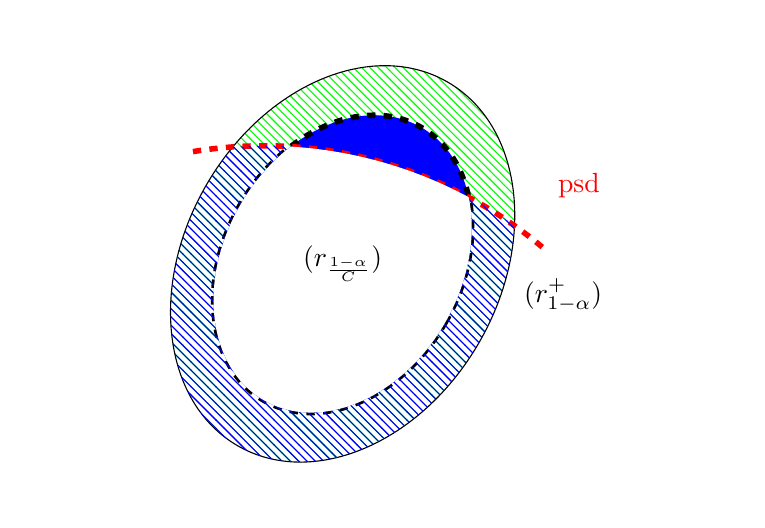
\begin{tikzpicture}[
  elip/.style={fill=white, line width=0},
  truncated/.style={pattern=north west lines, pattern color=blue},
  truncelip/.style={dashed, line width=2pt, fill=blue},
  rest/.style={pattern=north west lines, pattern color=green},
  psd/.style={dashed, color=red, line width=2pt}
]
  \clip (-4,-3) rectangle (5,3);

  \def\origelip{(0,0) ellipse [x radius=1.5, y radius=2, rotate=-30]}
  \def\truncatedelip{(0,0) ellipse [x radius=2, y radius=2.66666, rotate=-30]}

  \def\psdradius{5.5}
  \def\psdcircle{(psdcenter) [draw=none] circle (\psdradius)}
  \fill[rest]\truncatedelip;
  \draw[truncelip]\origelip;
  \draw\truncatedelip;

  \node at (-1,-4) (psdcenter) {};
  \node[color=red] at (3,1) {psd};

  \draw[psd] ([shift=(50:\psdradius)]psdcenter) arc (50:100:\psdradius);
  \begin{scope}
    \clip \psdcircle;
    \fill[truncated]\truncatedelip;
    \fill[elip] \origelip;
  \end{scope}

  \node at (0,0) {$\Eps(r_{\frac{1-\alpha}{C}})$};
  \node at (2.8,-.4) {$\Eps(r^+_{1-\alpha})$};
\end{tikzpicture}

  \caption{\label{fig:bayesian.r_separation}
    Same as Fig.~\ref{fig:bayesian.ellipsoids} (right).
    Note that the solid blue and hatched blue regions need to have the same volume.
  }
\end{figure}
%%%%%%%%%%%%%%%%%%%%%%%%%%%%%%%%%%%%%%%%%%%%%%%%%%%%%%%%%%%%%%%%%%%%%%%%%%%%%%%


Based on the gap proven in Lemma~\ref{lem:bayesian.positivity_violation}, we will now turn to the following question:
In case Eq.~\eqref{eq:bayesian.criterion} does not hold -- that is the corresponding ellipsoid is not fully contained in the psd states -- is the corresponding gap always large enough to be efficiently detectable?
\begin{lemma}\label{lem:bayesian.r_separation}
   Let $\vec a \in \mathbb{N}^d$ be an instance of the number partition problem and denote by $\Eps_{\vec{a}}$ the corresponding encoding ellipsoid as given by Eq.~\eqref{eq:bayesian.positivity_violation.ellipsoid}.
  Furthermore, denote by $\Pdf_{\varrho_0,\Sigma}$ the Gaussian density, which encodes $\Eps_{\vec{a}} = \Eps(r_\frac{\alpha}{C})$ as an $\frac{\alpha}{C}$ credible region as given by Lemma~\ref{lem:bayesian.encoded_ellipsoid}.
  Assume that $\vec a$ has a balanced sum partition and, therefore, $\Eps_{\vec{a}}$ is not a subset of $\States$.

  Then, there exists a polynomial $p$ such that
  \[
    {r^+_{\alpha}}^2 - {r_\frac{\alpha}{C}}^2 \ge 2^{-p(\log \norm{\vec a}_1)}.
  \]
  Here, $\norm{\vec a}_1 = \sum_k \abs{a_k}$.
  In words, the gap of violation of Eq.~\eqref{eq:bayesian.criterion} can only become polynomially small in the logarithm of the size of the problem specification.
\end{lemma}
\begin{proof}
  First, let us lower bound the volume of $\Eps(r_\frac{\alpha}{C})$ that lies outside the psd states (the solid blue region in Fig.~\ref{fig:bayesian.r_separation}).
  From Lemma~\ref{lem:bayesian.positivity_violation} we know, that there exists a $\varrho\in \Eps(r_\frac{\alpha}{C})$ with smallest eigenvalue smaller than $- \tilde p{(\norm{\vec a})}^{-1}$ for some polynomial $\tilde p$.
  This also gives us a lower bound on
  \[
    \mathrm{dist}(\varrho,\States) = \inf_{\varrho' \in \States} \norm{\varrho - \varrho'}_2.
  \]
  From~\cite[Theorem~III.2.8]{Bhatia_1997_Matrix} we know that for every $\varrho_+ \in \States$ the following bound holds:
  \[
    \begin{split}
      \norm{\varrho - \varrho_+}_2
      &\ge \norm{\varrho - \varrho_-}_\infty
      \ge \norm{\vec\lambda^\uparrow(\varrho) - \vec\lambda^\uparrow(\varrho_+)}_2 \\
      &\ge \abs{\mineig(\varrho) - \mineig(\varrho_+)}
      \ge \tilde p{(\norm{\vec a})}^{-1}.
    \end{split}
  \]
  Here, $\vec\lambda^\uparrow(\rho)$ denotes the vector of eigenvalues of $\rho$ in ascending order.
  Therefore,
  \[
    \label{eq:bayesian.r_separation.dist}
    \mathrm{dist}(\varrho,\States) \ge \tilde p{(\norm{\vec a})}^{-1}.
  \]
  This allows us to lower bound the volume of $\Eps(r_\frac{\alpha}{C})$ that lies outside the psd states by an ellipsoid with the same covariance, but radius ${(2\, \tilde p(\norm{\vec a}) \, \maxeig(\Sigma))}^{-1}$
  \begin{align}
    \label{eq:bayesian.r_separation.volume}
    \mathrm{Vol}\left( \Eps(r_\frac{\alpha}{C}) \setminus \States \right)
    &\ge \frac{\pi^{\Nhalf} \abs{\Sigma}}{\Gamma(\Nhalf + 1)} \, \frac{1}{{\left( 2 \tilde p(\norm{\vec a}) \, \maxeig(\Sigma) \right)}^{N}} \\
  \end{align}
  Furthermore, we have
  \[
    \label{eq:bayesian.r_separation.volume2}
    \mathrm{Vol}\left(\Eps(r^+_{1-\alpha}) \setminus \Eps(r_\frac{1-\alpha}{C}) \right)
    = \mathrm{Vol}\left( \Eps(r_\frac{1-\alpha}{C}) \setminus \States \right)
  \]
  since the solid blue and hatched blue regions in Fig.~\ref{fig:bayesian.r_separation} must be of same size.
  We now relate the volume inequality~\eqref{eq:bayesian.r_separation.volume} to a lower bound for the mass of the ellipsoid outside the psd states w.r.t.\ the Gaussian density:
  Due to the set of states $\States$ having finite radius $\sqrt{\tfrac{2(d-1)}{d}}$~\cite[Eq.~(18)]{Kimura_2003_Bloch}, we must have $r^+_{\alpha} \le 2 \sqrt{2}$.
  Therefore,
  \begin{align}
    P\left( \Nhalf, \tfrac{{r^+_{\alpha}}^2}{2} \right) - P\left( \Nhalf, \tfrac{{r_\frac{\alpha}{C}}^2}{2} \right)
    &= \frac{1}{ {(2\pi)}^{\frac{N}{2}} \, \abs{\Sigma}^{\frac{1}{2}} } \, \int_{\Eps(r^+_{\alpha}) \setminus \Eps(r_\frac{\alpha}{C})} \mathrm{e}^{-\frac{1}{2} \norm{\varrho - \varrho_0}^2} \dd^N \varrho \\
    &\ge \frac{\mathrm{e}^{-4}}{{(2\pi)}^{\frac{N}{2}} \, \abs{\Sigma}^{\frac{1}{2}}} \, \mathrm{Vol}\left(  \Eps(r^+_{\alpha}) \setminus \Eps(r_\frac{\alpha}{C})  \right) \\
    &\ge \frac{\mathrm{e}^{-4} \pi^{\Nhalf} \, \abs{\Sigma}^{\frac{1}{2}}}{2^\frac{N}{2} \Gamma(\Nhalf + 1)} \, \frac{1}{{\left( 2 \tilde p(\norm{\vec a}) \, \maxeig(\Sigma) \right)}^{N}} \\
    &=: 2^{-p(\log \norm{\vec a}_1) - 1}
    \label{eq:bayesian.r_separation.p_diff}
  \end{align}
  Finally, note that the following crude inequality
  \[
     P\left( \Nhalf, \tfrac{{r^+_{\alpha}}^2}{2} \right) - P\left( \Nhalf, \tfrac{{r_\frac{\alpha}{C}}^2}{2} \right)
     = \int_y^x \frac{t^{\Nhalf - 1} \ee^{-t}}{\Gamma(\Nhalf + 1)} \,\dd t \le x - y
  \]
  holds for $x \ge y$, since the integrand is less than 1.
  Therefore, with Eq.~\eqref{eq:bayesian.r_separation.p_diff}
  \[
    {r^+_{\alpha}}^2 - {r_\frac{\alpha}{C}}^2 \ge 2^{-p(\log \norm{\vec a}_1)},
  \]
  which proofs the claim.
\end{proof}


We now turn to the problem of computing the normalization constant $C$ for the restricted Gaussian distribution~\eqref{eq:bayesian.density_plus}.
First, we efficiently compute a credibility $\alpha' \in [0,1]$ such that the corresponding credible ellipsoid $\Eps(r_\frac{\alpha'}{C})$ is guaranteed to be contained in the psd states without knowing the value of $C$.
This allows us to leverage Eq.~\eqref{eq:bayesian.criterion} to compute $C$.

\begin{lemma}\label{lem:bayesian.always_contained}
  Let $\vec a \in \mathbb{N}^d$ be an instance of the number partition problem and denote by $\Eps_{\vec{a}}$ the corresponding encoding ellipsoid as defined by Eq.~\eqref{eq:bayesian.positivity_violation.ellipsoid}.
  Denote by $\Pdf_{\varrho_0,\Sigma}$ the Gaussian density, which encodes $\Eps_{\vec{a}}$ as an $\alpha$ credible region according to Lemma~\ref{lem:bayesian.encoded_ellipsoid}.
  Then, the ellipsoid $\Eps(r)$ is fully contained in the psd states provided
  \[
    \label{eq:bayesian.always_contained}
    r \le \sqrt{\frac{d}{2(d-1)}} \, \frac{\mineig\varrho_0}{\sqrt{\maxeig\Sigma}}
  \]
\end{lemma}
\begin{proof}
  We know that for any $\varrho \in \Eps(r)$ with $r$ fulfilling~\eqref{eq:bayesian.always_contained} the following inequalities hold
  \begin{align*}
    \norm{\varrho - \varrho_0}
    &\le \frac{1}{\sqrt{\mineig\Sigma^{-1}}}\, \norm{\varrho - \varrho_0}_\Sigma \\
    &\le \frac{1}{\sqrt{\mineig\Sigma^{-1}}}\, r \\
    &\le \sqrt{\frac{d}{2(d-1)}}\, \mineig \varrho_0.
  \end{align*}
  Here, we have used $\mineig\Sigma^{-1} = {(\maxeig \Sigma)}^{-1}$, which holds for any positive definite matrix $\Sigma$.
  Therefore, $\Eps(r) \subset \States$ due to Lemma~\ref{lem:ortho.spheres}.
\end{proof}


\begin{lemma}\label{lem:bayesian.normalization_constant}
  Using the same notation as Lem.~\ref{lem:bayesian.always_contained} and assuming Prob.~\ref{prob:bayesian.trucated_cr} can be solved efficiently.
  Then, for every instance $\vec a$ of the number partition problem consider the corresponding ellipsoid encoding distribution according to \cref{lem:bayesian.encoded_ellipsoid} with parameters $\theta, \Sigma$.
  Then, we can efficiently approximate the normalization constant $C$ of $\Pdf^+_{\theta,\Sigma}$ with exponentially small multiplicative error.
  More precisely, we have
  \[
    C = \tilde C (1 + \epsilon),
  \]
  where $\tilde C$ can be computed in polynomial time making the correction term $\epsilon$ exponentially small.
\end{lemma}
\begin{proof}
  Due to Lemma~\ref{lem:bayesian.always_contained} and $\mineig\theta > 0$, we can always find an $r > 0$ such that $\Eps(r)$ is fully contained in the psd.
  Indeed, the eigenvalues of $\theta$ and $\Sigma$ are readily calculated because of their particular simple form in Eq.~\eqref{eq:ellpos.rho0} and Lemma~\ref{lem:bayesian.encoded_ellipsoid}:
  \[
    \sqrt{\frac{d}{2(d-1)}} \, \frac{\mineig\theta}{\sqrt{\maxeig\Sigma}}
    =  \frac{q}{R_1 \sqrt{2d(d-1)}}
  \]
  Set\footnote{%
    Note that $\alpha$ does not denote the credibility used for encoding the ellipsoid in question, but an auxiliary ellipsoid used for computing $C$ here.
  }
  \[
    \alpha := P\left( \Nhalf, \tfrac{r^2}{2} \right).
  \]
  Since we can choose $r$ as small as we want, we may assume that $x = \frac{r^2}{2} \ll 1 < \Nhalf$.
  In this regime, we can expand the normalized incomplete $\Gamma$-function $P$ in a power series~\cite{Gil_2012_Efficient}
  \[
    \label{eq:bayesian.normalization_constant.incomplete_gamma}
    P\left( \Nhalf, x \right) = \frac{x^{\Nhalf} \ee^{-x}}{\Gamma\left( \Nhalf + 1 \right)} \sum_{k=0}^\infty \frac{x^k}{{\left( \Nhalf + 1 \right)}_k},
  \]
  where
  \[
    {\left( \Nhalf + 1 \right)}_k = \frac{\Gamma\left( \Nhalf + k + 1 \right)}{\Gamma\left( \Nhalf + 1 \right)}.
  \]
  Truncating the series in Eq.~\eqref{eq:bayesian.normalization_constant.incomplete_gamma} for $k \ge k_0$
  \[
    \label{eq:bayesian.normalization_constant.series}
    P\left( \Nhalf,x \right) = P_{k_0}\left( \Nhalf,x \right) + R_{k_0}\left( \Nhalf,x \right),
  \]
  with
  \[
    P_{k_0}\left( \Nhalf,x \right)
    = \frac{x^{\Nhalf} \ee^{-x}}{\Gamma\left( \Nhalf + 1 \right)} \sum_{k=0}^{k_0} \frac{x^k}{{\left( \Nhalf + 1 \right)}_k}
  \]
  we can derive a bound on the truncation error $R_{k_0}(\Nhalf,x)$~\cite[Eq.~(2.18)]{Gil_2012_Efficient}
  \[
    R_{k_0}(\Nhalf,x) \le \frac{x^{\Nhalf + k_0} \ee^{-x}}{\Gamma(\Nhalf + k_0 + 1)}\, \frac{\Nhalf + k_0}{\Nhalf + k_0 - x - 1}.
  \]
  Since $x \ll 1$, the term $x^{k_0}$ ensures that we can make the error in computing $\alpha$ exponentially small using only polynomial time in evaluating $P_{k_0}(\Nhalf, x)$.


  % Trace the error \delta -> error bound for r^+_{1-\alpha}
  Now, assume that we have computed $\tilde\alpha = \alpha-\epsilon$ for some truncation error $\epsilon = R_{k_0}(\Nhalf,x) > 0$.
  We may now use the postulated efficient algorithm for Prob.~\ref{prob:bayesian.trucated_cr} to compute the radius of the manifestly positive MVCR $r^+_{\tilde\alpha}$ and, hence, using Eq.~\eqref{eq:bayesian.criterion} the normalization constant:
  Since $C>1$, we have with $r_{\alpha} = r$
  \[
    r_\frac{\tilde\alpha}{C} = r_\frac{\alpha-\epsilon}{C} < r_{\alpha} \implies \Eps(r_\frac{\tilde\alpha}{C}) \subset \States \implies r_\frac{\tilde\alpha}{C} = r^+_{\tilde\alpha} \le r_{\alpha}.
  \]
  Therefore, the ellipsoid with radius $r^+_{\tilde\alpha}$ is also contained in the psd states.
  The same holds true if we replace $r^+_{\tilde\alpha}$ by the actual output $r^+_{\tilde\alpha} \pm \delta$ of the postulated efficient algorithm for Prob.~\ref{prob:bayesian.cr}
  Here, $\delta$ denotes the accuracy that is part of the input to the problem of computing $r^+_{\tilde\alpha}$.
  By choosing $\delta$ small enough and possibly replacing the original radius $r$ by $r - \delta$, we can ensure that
  \[
    \label{eq:bayesian.normalization_constant.small_enough_r}
    \Eps(r^+_{\tilde\alpha} \pm \delta) \subset \States,
  \]
  as well.
  Therefore, Eq.~\eqref{eq:bayesian.criterion} holds and we find
  \begin{align}
    \label{eq:bayesian.normalization_constant.almost_c}
    \frac{\tilde\alpha}{C}
    &= P\left( \Nhalf, \tfrac{{r^+_{\tilde\alpha}}^2}{2} \right) \\
    &= P\left( \Nhalf, \tfrac{{(r^+_{\tilde\alpha} \pm \delta)}^2}{2} \right) - \frac{1}{\Gamma(\Nhalf)} \int_{\tfrac{{r^+_{\tilde\alpha}}^2}{2}}^{\tfrac{{(r^+_{\tilde\alpha} \pm \delta)}^2}{2}}\, t^{\Nhalf - 1} \ee^{-t} \dd t.
  \end{align}
  The first addend on the right hand side can be evaluated using the same series expansion as in Eq.~\eqref{eq:bayesian.normalization_constant.series}, since we are in the same regime $\tfrac{{r^+_{\tilde\alpha}}^2}{2} \ll \Nhalf$.
  The second addend can be bounded by
  \[
    \label{eq:bayesian.normalization_constant.upper_bound}
    \Abs{\frac{1}{\Gamma(\Nhalf)} \int_{\tfrac{{r^+_{\tilde\alpha}}^2}{2}}^{\tfrac{{(r^+_{\tilde\alpha} \pm \delta)}^2}{2}}\, t^{\Nhalf - 1} \ee^{-t} \dd t}
    < \frac{\left( 2 {r^+_{\tilde\alpha}} \delta + \delta^2 \right)}{2}
  \]
  since
  \[
    \frac{t^{\Nhalf - 1} \ee^{-t}}{\Gamma(\Nhalf)} < 1.
  \]
  Let us assume w.l.o.g.\ $r^+_{\tilde\alpha} \le 1$.
  This bound, as well as the error bound $\epsilon' > 0$ for the finite series-evaluation of $P$ in~\eqref{eq:bayesian.normalization_constant.almost_c} leads to
  \[
    \frac{\tilde\alpha}{C} = P_{k_0}\left( \Nhalf, \tfrac{{(r^+_{\tilde\alpha} \pm \delta)}^2}{2} \right) + \epsilon' \pm D \delta
  \]
  for some appropriate constant $D$.
  A little arithmetic gives
  \[
    \label{eq:bayesian.normalization_constant.formula_c}
    C = \frac{\tilde\alpha}{P_{k_0}(\ldots)} \, \left( 1 - \frac{\epsilon' \pm D\delta}{P_{k_0}(\ldots) + \epsilon' \pm D\delta} \right).
  \]
  By assumption we can make both $\epsilon'$ and $\delta$ exponentially small using only polynomial time
  Furthermore, $P_{k_0}(\Nhalf, x) \uparrow P(\Nhalf,x)$ for $k_0 \to \infty$ and the correction to
  \[
    \tilde C = \frac{\tilde\alpha}{P_{k_0}\left( \Nhalf, \tfrac{{(r^+_{\tilde\alpha} \pm \delta)}^2}{2} \right)}
  \]
  in Eq.~\eqref{eq:bayesian.normalization_constant.formula_c} can be made exponentially small using polynomial time.
  On the other hand, $\tilde C$ can be computed in polynomial time as well.
\end{proof}

We now have all the necessary parts for the proof of the main theorem~\ref{thm:bayesian.hardness}, which concludes this section.

\begin{proof}[Proof of Thm.~\ref{thm:bayesian.hardness}]
  The proof follows the outline stated in the main text:
  First, we encode the ellipsoid of Problem~\ref{prob:ortho.ellpos} to be checked as a MVCR of a Gaussian with mean $\varrho_0$ and covariance matrix $\Sigma$ according to Lemma~\ref{lem:bayesian.encoded_ellipsoid}.
  Using Lemma~\ref{lem:bayesian.normalization_constant}, we compute an estimate $\tilde C$ to the normalization constant $C$.
  Using the techniques from the proof of the aforementioned Lemma, we may compute an estimate
  \[
    \alpha = C \, P\left( \Nhalf, 1 \right) = \tilde C (1 + \epsilon) \left( P_{k_0}\left( \Nhalf, 1 \right) + \epsilon' \right) = \tilde\alpha + \epsilon''.
  \]
  This can be done for exponential small errors $\epsilon, \epsilon'$ in polynomial time.
  Here, the computable value is given by
  \[
    \tilde\alpha = \tilde C \, P_{k_0}\left(\Nhalf, 1 \right).
  \]
  An exponential small difference of $\alpha$ and $\tilde\alpha$ also implies an exponential small difference of $r^+_{1-\alpha}$ and $r^+_{\tilde\alpha}$:
  Set $x := r^+_{\alpha}$ and $\tilde x := r^+_{\tilde\alpha}$ and assume $x > \tilde x$ -- the opposite case can be treated along the same lines by choosing a larger constant as a bound for $\tilde x$.
  Following Eq.~\eqref{eq:bayesian.r_separation.p_diff}, we have
  \begin{align*}
    P\left( \Nhalf, \tfrac{x^2}{2} \right) - P\left( \Nhalf, \tfrac{{\tilde x}^2}{2} \right)
    &\ge \frac{\mathrm{e}^{-4}}{{(2\pi)}^{\frac{N}{2}} \, \abs{\Sigma}^{\frac{1}{2}}} \, \mathrm{Vol}\left(  \Eps(x) \setminus \Eps(\tilde x)  \right) \\
    &= \frac{\mathrm{e}^{-4}}{2^{\Nhalf} \Gamma(\Nhalf + 1)} \left( x^N - {\tilde x}^N \right).
  \end{align*}
  Since for fixed $N$, the left hand side can be made exponentially small in polynomial time by improving $\tilde\alpha$, so can the right hand side.
  Therefore, the difference $\abs{x - \tilde x}$ can be made exponentially small as well.


  Now, choose the errors $\epsilon$ and $\epsilon'$ in such a way that
  \[
    \abs{r^+_{\alpha} - r^+_{\tilde\alpha}} \le \frac{\Delta}{4}.
  \]
  Here, $\Delta = 2^{-p(\log \norm{\vec a}_1)}$ is the (at worst exponentially small) gap from Lemma~\ref{lem:bayesian.r_separation}.
  Furthermore, we run the algorithm for computing $r^+_{\tilde\alpha}$ with precision $\delta = \frac{\Delta}{4}$ and denote the result by $\tilde r$.
  If $\abs{\tilde r - \sqrt{2}} \le \frac{\Delta}{2}$, we know that $r^+_{\alpha} = r_\frac{\alpha}{C}$ and the ellipsoid is fully contained in the psd states.
  Otherwise we know that it is not.
\end{proof}


%%%%%%%%%%%%%%%%%%%%%%%%%%%%%%%%%%%%%%%%%%%%%%%%%%%%%%%%%%%%%%%%%%%%%%%%%%%%%%%
\printbibliography[heading=bibintoc]

\end{document}
